%% PNAStwoS.tex
%% Sample file to use for PNAS articles prepared in LaTeX
%% For two column PNAS articles
%% Version1: Apr 15, 2008
%% Version2: Oct 04, 2013

%% BASIC CLASS FILE

\documentclass[10pt,letterpaper]{article}

\usepackage{setspace}
%\doublespacing
\usepackage{geometry}

\geometry{letterpaper, margin=1in}
%\usepackage{times}
\usepackage{pslatex}
\usepackage{apacite}
\usepackage{url}
\usepackage{graphicx}
\usepackage{caption}
\usepackage{subcaption}
\usepackage{listings}
\usepackage{color}
\usepackage{textcomp}
\usepackage{amsmath}
\usepackage{amssymb}
\usepackage{wrapfig}
\usepackage{lipsum}


\graphicspath{{../figures/}}

\def\signed #1{{\leavevmode\unskip\nobreak\hfil\penalty50\hskip2em
  \hbox{}\nobreak\hfil(#1)%
  \parfillskip=0pt \finalhyphendemerits=0 \endgraf}}

\newsavebox\mybox
\newenvironment{aquote}[1]
  {\savebox\mybox{#1}\begin{quote}}
  {\signed{\usebox\mybox}\end{quote}}


 \newcommand{\denote}[1]{\mbox{ $[\![ #1 ]\!]$}}

\definecolor{Red}{RGB}{255,0,0}
\newcommand{\red}[1]{\textcolor{Red}{#1}}  
\definecolor{Green}{RGB}{10,200,100}
\definecolor{Blue}{RGB}{10,100,200}
\newcommand{\ndg}[1]{\textcolor{Green}{[ndg: #1]}}  
\newcommand{\mht}[1]{\textcolor{Blue}{[mht: #1]}}  

\usepackage{titlesec}

\setcounter{secnumdepth}{4}

\titleformat{\paragraph}
{\normalfont\normalsize\bfseries}{\theparagraph}{1em}{}
\titlespacing*{\paragraph}
{0pt}{3.25ex plus 1ex minus .2ex}{1.5ex plus .2ex}

\title{A pragmatic theory of generic language}
%\title{Generics are vague: A formal theory of generalizations in language}
%\title{Generics are vague: a probabilistic model of generic language}
%\title{Generic language is vague yet rationally understood}
%\title{Generic language is vague yet pragmatically understood}
%\title{Generic language is vague yet pragmatically used}

\author{{\large \bf Michael Henry Tessler} (mtessler@stanford.edu)\\ {\large \bf Noah D. Goodman} (ngoodman@stanford.edu) \\
  Department of Psychology, Stanford University}
  
 \date{}

\begin{document}

\maketitle

%\contributor{Submitted to Proceedings of the National Academy of Sciences
%of the United States of America}

%%%Newly updated.
%%% If significance statement need, then can use the below command otherwise just delete it.

%
%\significancetext{
%Understanding the world requires making generalizations about categories; we use generic language to convey such generalizations: `dogs bark', `rats carry disease', and `liberals drink lattes'.
%These simple sentences are common in ordinary conversation, child-directed speech, and political discourse.
%They are how we teach, how we motivate, and how we persuade (or mislead) others.
%Yet the precise meaning of generics is a puzzle that has resisted formalization.
%We introduce a mathematical model of generic language by combining principles of language understanding with a basic meaning in terms of property statistics.
%This theory provides the connective tissue between generic language and conceptual knowledge and gives insight into how everyday language use is tied to beliefs. 


%of the parties involved.
%
%Understanding the world requires making generalizations about categories.
%Generic language (e.g. \emph{Dogs bark.}) provides an efficient and ubiquitous way to transmit this kind of information.
%Yet, these common, simple sentences that even 2-year-olds can comprehend have philosophically puzzling qualities which have impeded precise formalization. 
%We explain the apparent paradoxes using a meaning of generic language that is simple but underspecified. 
%With uncertainty in the language, general principles of communication and 
%interlocutors' shared beliefs about the categories and properties in question 
%are responsible for establishing a precise meaning in context.
%This theory provides the connective tissue between generic language and conceptual knowledge and demonstrates 
% how beliefs play a foundational role in understanding language. 
 %
 % We find this model to explain almost all of the variance in human judgments of the acceptability of familiar generic sentences and 
% to human interpretations of unfamiliar generic sentences.
%to others forms the fabric of conceptual developmental and cultural transmission.
%Utterances that convey generalizations----generic utterances----are ubiquitous in everyday conversational and child-directed speech, 
%yet there is to date no formal account of their precise meanings.
%Humans build internal representations of the world by making generalizations about categories, and use language to convey these generalizations to 
%M.H.T. and N.D.G developed theory and designed research; M.H.T. performed research and analyzed data. M.H.T. and N.D.G. wrote the paper.
%}

%\maketitle

\begin{abstract}
{Generalizations about categories are central to human understanding, and generic language (e.g.~\emph{Dogs bark.}) provides a simple and ubiquitous way to communicate these generalizations. 
Yet the meaning of generic language is philosophically puzzling and has resisted precise formalization.
We explore the idea that the core meaning of a generic sentence is simple but underspecified, 
and that general principles of pragmatic reasoning are responsible for establishing the precise meaning in context.
Building on recent probabilistic models of language understanding, we provide a formal model for the evaluation and comprehension of generic sentences. 
This model explains the puzzling flexibility in usage of generics in terms of diverse prior beliefs about properties.
We elicit these priors experimentally and show that the resulting model predictions explain almost all of the variance in human judgments for both common and novel generics.
This theory provides a mathematical bridge between the words we use and the concepts they describe.
}
\end{abstract}

%\keywords{generic language | semantics | pragmatics | categories}

%\abbreviations{SAM, self-assembled monolayer; OTS, octadecyltrichlorosilane}

Most would agree that \emph{Swans are white}, but certainly not every swan is.
%Imagine talking with a 2-year-old about the color red.
%Colors are difficult to describe because they take shape in different physical forms and the function of color is abstract.
%You might offer the toddler something generic like, ``Apples are red.''. 
%Few would argue with the truth of this sentence, yet its precise meaning is difficult to specify. 
This type of utterance conveys a generalization about a category (i.e. \textsc{swans}) and is known as a generic utterance \cite{Carlson1977,Leslie2008}.
It is believed that every language can express generic meaning \cite{Behrens2005,Carlson1995}, and that generics are essential to the growth of conceptual knowledge \cite{Gelman2004} and how kinds are represented in the mind \cite{Leslie2008}.
Generic language is ubiquitous in everyday conversation as well as in child-directed speech \cite{Gelman2008}, and children as young as two or three understand that generics refer to categories and support generalization \cite{Cimpian2008}.
% and though English and many other languages do not possess an unambiguous form devoted to generic meaning \cite{Behrens2000, AlMalki2014}. 
Additionally, generics are the primary way by which speakers discuss social categories, making them key to propagating stereotypes \cite{GelmanEtAl2004,Rhodes2012,Leslie2015} and impacting motivation \cite{Cimpian2010motivation}.
Despite their cognitive centrality and apparent simplicity, a formal account of generic meaning remains elusive.

One major hurdle to formalizing generic language arises in the conditions by which a generic sentence is true.
At first glance, generics seem like universally-quantified statements as in \emph{All swans are white}, but unlike universals, generics are resilient to counter-examples (e.g. black swans). 
Interpreting the generic as meaning ``most'' (i.e. \emph{Most swans are white}) captures many cases, but cannot explain why \emph{Robins lay eggs} and \emph{Mosquitos carry malaria} are so intuitively compelling: Only adult female robins lay eggs and a very tiny fraction of mosquitos actually carry malaria.
Indeed, it appears that any explanation in terms of how common the property is within the kind violates intuitions --- for the robins, laying eggs is practically synonymous with being female (i.e., the properties are present in the same proportion), yet \emph{Robins are female} is not a reasonable utterance while \emph{Robins lay eggs} is fine.

% as , even though the two properties are present in the same proportion (about 50\%) in the category of robins.
%\ndg{No precise meaning formalized in the mathematical language of logic seems to be sufficient to capture the meaning of natural language generics.}

%Generics are additionally puzzling in how they are interpreted. 
The mystery deepens with how novel generics are interpreted.
%The strong interpretation of novel generics deepens the mystery.
While \emph{Mosquitos carry malaria} suggests the generic must in some way be analogous to ``some'' (i.e. \emph{Some swans are white.}), generics are often interpreted as implying the property is widespread within the kind:
%Yet generics often imply the property is widespread: 
%Listeners often interpret a novel generic as applying to \emph{nearly all} of a category 
Consider the difference between \emph{Some swans have hollow bones} to \emph{Swans have hollow bones} \cite{Gelman2002}.
When asked how common a property would need to be for the generic utterance to be true, both children and adults require the property to be less widespread than they infer when just told the generic \cite{Cimpian2010,Brandone2014}, suggesting that communicating with generics can exaggerate evidence.
%Both children and adults believe the generic implies the property-in-question is even more widespread than when asked how common the property would need to be for the generic to apply

How can generics have such flexible truth conditions while simultaneously having strong implications?
In this paper we offer a mathematical model of generic language in terms of pragmatic inference of the degree of prevalence required to assert a generic.  
We show that this model predicts the patterns in human endorsement of familiar generic sentences and interpretation of novel generics. 

\section*{Computational method}


Generics express a relation between a kind (e.g. \textsc{robins}) and a property (e.g. \textsc{lays eggs}). 
Semantic accounts of generics are usually given by appealing to either the statistics of the world (e.g. \emph{Barns are red} because most barns are) or to structured, conceptual representations (e.g. \emph{Bishops move diagonally} not because most bishops do but because the laws of chess dictate that they do) \cite{Carlson1995essay}. 
This latter perspective emphasizes the structure of generic knowledge \cite{Prasada2000}, and views generic utterances as the way of expressing special mental relationships between kinds and properties \cite{Leslie2008, Prasada2012}. The puzzles of generic language then reduce to puzzles about mental representation of kind-property relations.

However, generic language is not unique in its flexibility.
Language understanding in general depends on assumptions interlocutors make about each other, which can result in meanings interpreted with a complex sensitivity to context \cite{Clark1996,Grice1975,Levinson2000}, recently formalized in probabilisitic models of language understanding---the Rational Speech Acts (RSA) theory \cite{Frank2012,Goodman2013}. 
Perhaps then, the puzzles of generic language can be partly understood as effects of pragmatic reasoning.
If this is the case, then a relatively simple semantic theory, phrased in terms of statistical regularities in the world, could be enough to formalize generic language.
Abstract, mental representations may still operate; yet we suggest generic language requires the currency of generalization: probability. 

For a given kind $K$ (e.g.~\textsc{robins}) and property $F$ (e.g.~\textsc{lays eggs}), we refer to the probability that an object of kind $K$ has property $F$, that is $P(F\mid K)$, as the \emph{prevalence} of $F$ within $K$.\footnote{Because we aim to explain the psycholinguistics of generics, we are generally interested in the subjective probability, not the actual frequency in the world.}
Logical quantifiers can be described as conditions on prevalence (i.e.~\emph{some} is $P(F\mid K)>0$, \emph{all} is $P(F\mid K)=1$). 
Extending this, it seems the simplest meaning for generic statements would be a similar threshold on prevalence: $P(F\mid K)>\tau$ \cite{Cohen1999}. 
However, no fixed value of the threshold, $\tau$, would allow for the extreme flexibility generics exhibit (e.g. \emph{Robins lay eggs} vs. \emph{Robins are female}; \emph{Mosquitos carry malaria}).% simultaneously with the interpretations of some novel generics being strong. 



We suggest that this threshold is not a fixed property of the language, but is established by pragmatic inference.
This inference depends on property and category knowledge, but is otherwise a general mechanism of language not specific to interpreting generic statements.
We follow the treatment of RSA applied to vague adjectives (e.g.~\emph{tall}), using an underspecified threshold criterion \cite{Lassiter2013,Lassiter2015}. % who have extended RSA to explain vague adjectives (e.g.~\emph{tall}) in terms of an underspecified threshold criterion. %(Cf.~\citeA{Qing2014}). 
%We follow this treatment, adopting as the underlying scale the property prevalence.
We imagine a hypothetical, pragmatic listener ($L_1$) concerned with learning the prevalence of a certain property in a certain category, $x=P(F \mid K)$, who reasons about an informative speaker ($S_1$), who in turn reasons about a literal listener ($L_0$):
\begin{eqnarray}
P_{L_{1}}(x , \tau \mid u) &\propto& P_{S_{1}}(u \mid x, \tau) \cdot P(x) \cdot P(\tau) \label{eq:L1}\\
P_{S_{1}}(u \mid x, \tau) &\propto&  {P_{L_{0}}(x \mid u, \tau)}^{\lambda} \label{eq:S1}\\
P_{L_{0}}(x \mid u, \tau) &\propto& {\delta_{\denote{u}(x, \tau)} P(x)}. \label{eq:L0}
\end{eqnarray}




%hears an utterance $u$, which is either a generic statement (e.g.~\emph{Robins lay eggs.}) or an uninformative \emph{null} utterance\footnote{In this case, the other thing the speaker could have done (but didn't) is said nothing, the \emph{null} utterance. 
%All results reported are similar when the alternative utterance is stipulated to be the negation---\emph{It is not the case that robins lay eggs.}---or the generic of the negation---\emph{Robins do not lay eggs.}---as opposed to the \emph{null} utterance.}.

 %generic utterance (\emph{Ks have F.}) from the speaker $S_{1}$ (Eq. \ref{eq:S1}). 
The pragmatic listener $L_1$ is trying to resolve how common F is within K (i.e.~$x = P(F\mid K) \in [0, 1]$); 
she does so by considering both what she knows about property F in general---her prior distribution $P(x)$ over prevalence of F---and her intuitive theory of the speaker $S_{1}$ as an informed and helpful interlocutor (Eq. \ref{eq:S1}).
$L_1$ assumes the meaning of the generic utterance expresses something about how common the property is (she knows it is a threshold on prevalence), but doesn't know exactly what it conveys (she has uncertainty about the threshold: $\tau \sim \text{Uniform([0,1])}$).
She believes the speaker $S_1$ knows what $\tau$ is, and is trying to be informative about the prevalence $x$ to the listener he is thinking about---an idealized literal listener ($L_{0}$, Eq. \ref{eq:L0}).
The literal listener too has access to the threshold $\tau$, and simply restricts her prior beliefs to situations where the truth-functional denotation of the utterance, $\denote{u}$, is true.

Pragmatic interpretation of language assumes the production of an utterance was a deliberate decision on behalf of the speaker, who could have said other things but didn't. 
We model generic language interpretation by $L_{1}$ (Eq. \ref{eq:L1}) as a pragmatic process resulting from the generic utterance (e.g.~\emph{Robins lay eggs.}) being produced by a speaker $S_{1}$ (Eq. \ref{eq:S1}), who had the alternative of not saying anything. 
We model this alternative by a \emph{null} utterance, which carries no information\footnote{
The \emph{null} utterance produces in a listener a posterior distribution identical with the prior. 
In this way, the contrast of the \emph{null} utterance alternative gives the generic speech-act substance.
This alternative can be realized in at least two other ways: the speaker could have said the negation of the utterance (i.e. \emph{It is not the case that robins lay eggs.}) or the negative generic (i.e. \emph{Robins do not lay eggs.}).
All results reported are similar for these two alternatives, and we use the alternative of the \emph{null} utterance for simplicity of demonstration.}.
The generic utterance has a threshold semantics, $\denote{\text{K F}}(x, \tau)=x>\tau$; while the null utterance is always true, $\denote{null}(x, \tau)=T$.
We further assume that the listener construes the utterance she has heard as a generic utterance (i.e. \emph{Birds, as a kind, lay eggs.}) as opposed to a specific (i.e. \emph{There are some birds right now laying eggs.}).
This \emph{identification} process is itself likely a result of pragmatic inference \cite{Cimpian2008}, which we do not attempt to model here. 
The fundamental question we address is: What is denotation of a generic utterance?



Example interpretation distributions for $P_{L_{1}}(x , \tau \mid u)$ upon hearing a generic utterance can be seen in Figure \ref{fig:priors1a}. 
Also shown are the corresponding prior beliefs, $P(x)$, about the prevalence of the property (which are also the posteriors upon hearing the null utterance).
We see that the interpretation of the generic depends a great deal on the shape of the prior.
When the prior is very left-skewed as in the case of \textsc{carries malaria}, then $\tau$ can plausibly be quite low while still being informative, since a low threshold still rules out many possible alternative kinds (and their corresponding degree of prevalence).
If the prior is right-skewed (e.g. \textsc{doesn't attack swimmers}), even an intermediate threshold would not result in an informative utterance (as not many kinds would be ruled out), and so the generic is unlikely to be used by speaker $S_1$ unless the property is practically-universal within the target category. 
Priors for properties that are unimodal with low variance (e.g. \textsc{is female}) are present in every kind in almost exactly the same proportion and thus are too obvious and certain to allow for a realistic, informative utterance: The posterior is not very different from the prior. 

The pragmatic listener $L_1$ (Eq.~\ref{eq:L1}) is a model of generic interpretation: Upon hearing a generic, what prevalence is a listener likely to infer?
We can now imagine a speaker $S_2$ who reasons about this type of listener: 
%$S_2$ knows some prevalence $x$ and is trying to decide whether or not to produce a generic to describe it to $L_1$.

\begin{equation} 
P_{S_{2}}(u \mid x) \propto  \int_{\theta} P_{L_{1}}(x , \tau \mid u) % =  P_{L_{1}}(x \mid u)
\label{eq:S2}
\end{equation}

Speaker $S_2$ is a model of felicity or truth judgments \cite{Degen2014}.
The speaker considers the thought-processes of listener $L_1$ (Eq.~\ref{eq:L1}) and decides if the generic is a good (albeit, vague) way to describe the prevalence $x$. 
$S_2$'s decision is with respect to the alternative of saying nothing: He will choose to produce the generic when the true prevalence $x$ is more likely under $L_1$'s posterior than under her prior. 
Critically, speaker $S_{2}$ doesn't actually know what the generic means (i.e. doesn't have access to the threshold $\tau$), but knows that $L_{1}$ will have to consider it, and integrates over the likely values she'll consider.
%We use $S_{2}$ (Eq.~\ref{eq:S2}) to model


%\subsection*{The structure of prevalence priors}

\section*{Empirical puzzle 1: Generics have flexible truth conditions}

\section*{Experiment 1a: The structure of prevalence priors}



 The prior $P(x)$ (in Eqs.~\ref{eq:L1}, \ref{eq:L0}) describes the belief distribution on the prevalence of a given property (e.g. \textsc{lays eggs}) across relevant categories. 
The shape of this distribution affects model predictions, but may vary significantly among different properties.
 We measured it empirically for a set of properties (e.g. \textsc{lays eggs, carries malaria}; 21 in total) that give rise to interesting generics (described below). 
 
\subsection*{Method}

\subsubsection*{Participants}
We recruited 60 participants over Amazon's crowd-sourcing platform Mechanical Turk (MTurk).  
Participants were restricted to those with US IP addresses and with at least a 95\% MTurk work approval rating (same for all experiments reported). 
%3 participants where unintentionally allowed to do the experiment for a second time; we excluded their second responses (resulting in $n=57$).
%2 participants self-reported a native language other than English; removing their data ($n=55$) has no effect on the results reported. 
%The experiment took about 10 minutes and participants were compensated \$1.00.

\subsubsection*{Procedure and materials}
On each trial of the experiment, participants filled out a table where each row was an animal category and each column was a property. 
Half of the animal categories were randomly selected from a set corresponding to the generics used in Expt. 1b (e.g. \textsc{robins, mosquitos}); the other half were self-generated by the participant.
%The experiment in full can be viewed at http://stanford.edu/~mtessler/experiments/generics/experiments/real-kinds/prior-2.html.
Participants were asked to fill in each row with the percentage of members of each of the species that had the property (e.g. ``50\%'').
Each participant reported on 16 properties (see {\it SI Section A} for more details).
 
 We used a set of properties associated with generics of theoretical interest (21 properties in total), motivated by conceptual distinctions pointed out by \citeA{Prasada2013}. 
The conceptual categories used to generate the properties (and their corresponding generics in Expt.~1b) were: majority characteristic (e.g. \emph{have spots}), minority characteristic (e.g. \emph{have manes}), striking (e.g. \emph{attack swimmers.}), and majority false generalizations (e.g. \emph{are female.}) \cite{Prasada2013}.
For a full list of the properties, and generic sentences used in Expt.~1b, see Table S1.
 
 \subsection*{Data analysis and results}
 
While each $P(x)$ is a single distribution on prevalence, it may be structured as the result of deeper conceptual knowledge. 
For instance, if participants believe that some kinds have a causal mechanism that \emph{could} give rise to the property, while others do not, then we would expect $P(x)$ to be structured as a mixture distribution (cf. \cite{Griffiths2005}).
If a kind can have the property, we assume the prevalence follows a Beta distribution with mean $\gamma$ and concentration $\xi$. 
If a kind cannot, the prevalence can only be 0\%.
The relative contribution of these two components is governed by mixture parameter $\theta$, inferred from the data.

\begin{align*}
	d_{observed} & \sim \begin{cases}
				 \text{Beta}(\gamma, \xi) & \mbox{if } \text{Bernoulli}(\theta) = \textsc{t}  \\
				 \delta_{x=0} & \mbox{if }\text{Bernoulli}(\theta) = \textsc{f} \\
				\end{cases} \\
	 d_{observed} &  \sim \theta \cdot \beta(\gamma,\xi)+ (1 - \theta) \cdot \delta_{x=0} 
\end{align*}

We put uninformative priors over all the parameters, $\theta \sim \text{Uniform}(0,1)$, 
$\gamma \sim \text{Uniform}(0,1)$, $\xi \sim \text{Uniform}(0, 50)$, and implemented these Bayesian statistical models using the probabilisitic programming language WebPPL \cite{dippl}. This statistical model reproduces the prior elicitation data with a low reconstruction error ($r^2 = 0.94$; see {\it SI Fig. 1}), strongly supporting the assumption of a structured prior. 

%
%We assume that \emph{when the property is possible}, its prevalence is distributed according to a Beta distribution with mean $\gamma$ and concentration $\xi$: 
%$P(x)=\theta \cdot \beta(\gamma,\xi)(x) + (1-\theta) \cdot \delta_{x=0}$.\footnote{This is similar in spirit to Hurdle Models of epidemiological data, where the observed counts of zeros is substantially greater than one would expect from standard models, such as the Poisson (e.g. adverse events to vaccines)\cite{hurdleModels}.}
%Thus, $\theta$ is the potential of a property to be present in a kind and $\gamma$ is the mean prevalence of the property among the kinds with the potential to have it. 
%
%We will describe the analysis model from the perspective of inferring the distribution of a particular property (e.g. \textsc{lays eggs}). 
%The same general structure is implemented for each item independently. 
%As well, we describe the models for Expt.~1a and ~2a together, as they use the same structure. 
%%We hypothesized that the prior elicitation task has an important latent structure. 
%For Expt.~1a, participants are asked to report the percentage of a kind with the property, for several different kinds of animals.
%Kinds can be divided into those that can have property and those that cannot.
%The relative contribution of these two components is governed by mixture parameter $\theta$, inferred from the data.
%Overall: 
%$ d_{observed}   \sim \theta \cdot \beta(\gamma,\xi)+ (1 - \theta) \cdot \delta_{x=0} $.
%
%%\begin{minipage}{0.5 \textwidth} \small
%\begin{align*}
%	d_{observed} & \sim \begin{cases}
%				 \text{Beta}(\gamma, \xi) & \mbox{if } \text{Bernoulli}(\theta) = \textsc{t}  \\
%				 \delta_{x=0} & \mbox{if }\text{Bernoulli}(\theta) = \textsc{f} \\
%				\end{cases} \\
%	 d_{observed} &  \sim \theta \cdot \beta(\gamma,\xi)+ (1 - \theta) \cdot \delta_{x=0} 
%\end{align*}
%%\end{minipage}
%%
%For Expt.~2a, participants are asked questions directly targeting $\theta$ and $\gamma$ in the above model (see {\it Expt. 2a}).
%We assume these two measurements follow a Beta distribution:\\
%%
%%\begin{minipage}{0.5 \textwidth} \small
%\begin{align*}
%d_{potential} &\sim \text{Beta}(\gamma_{potential}, \xi_{potential}) \\
%d_{expected} &\sim \text{Beta}(\gamma_{expected}, \xi_{expected}) 
%\end{align*}
%%\end{minipage}
%%
%To construct single prevalence distributions, $P(x)$, we generate $\theta$ from the posterior predictive distribution of $d_{potential}$ and use the same structure as in Expt.~1a.
%%\begin{minipage}{0.5 \textwidth} \small
%\begin{align*}
%\theta & \sim \text{Beta}(\gamma_{potential}, \xi_{potential}) \\ 
%%x & \sim \begin{cases} 
%%		\text{Beta}(\gamma_{expected}, \xi_{expected}) &\mbox{if } \text{Bernoulli}(\theta) = \textsc{t} \\
%%				\delta_{x=0} &\mbox{if } \text{Bernoulli}(\theta) = \textsc{f} \\
%%		\end{cases} \\
%x	 &  \sim \theta \cdot \beta(\gamma_{expected},\xi_{expected}) + (1-\theta)  \cdot \delta_{x=0}
%\end{align*}
%\end{minipage}


%We used the Metropolis-Hastings algorithm to estimate the posterior distribution over the latent parameters $\theta, \gamma$, and $\phi$ with 3 MCMC chains of 100,000 iterations removing the first 50,000 iterations.

%Intuition suggests that, for a given property (e.g. \textsc{lay eggs}), kinds fall into two distinct categories: those for which the property is possible (e.g. \textsc{ducks}) and those for which the property is impossible (e.g. \textsc{lions}).
%We hypothesized that participants' responses were structured in such a way as to be generated from a mixture of two distributions---$P_{present}(x)$ and $P_{absent}(x)$--- with mixture parameter $\theta$.
%$P_{present}(x)$ is comprised of the animal kinds for which the property is present (i.e. prevalence greater than 0\%), and we assume participants' responses are sampled from a Beta distribution with unknown mean $\gamma$ and concentration $\delta$. 
%$P_{absent}(x)$ corresponds to the animal kinds for which the property is absent (i.e. prevalence equal to 0\%), and the distribution we assume is a delta function at 0\% prevalence\footnote{This is similar in spirit to Hurdle Models of epidemiological data where the observed counts of zeros is greater than one would expect from standard models of count data such as the Poisson model \cite<e.g. adverse events to vaccines; >{hurdleModels}.}.


% Figure \ref{fig:priors1a} (insets) shows five example elicited prior distributions.


Using this structure, we can explore our 21 properties:
Figure \ref{fig:priors1a} shows the estimated mixture-parameter $\theta$ (the potential of the property to be present in a kind) and the mean prevalence when the property is present, $\gamma$. 
We see significant diversity among these properties in both dimensions, resulting in priors over prevalence with dramatically different shapes ( insets). 
This diversity matters because the model predictions for generic interpretation and felicity depend on the shape of the prior distribution (insets show example interpretation posteriors).
Lowering $\theta$ effectively makes the property more distinctive by increasing the relative probability mass at 0\%; this relaxes the truth conditions by making a lower threshold more informative.
Increasing $\gamma$ means the property is expected to be present in more members of the category; this tends to make truth conditions stricter, by reducing the range of prevalence values higher than the prior expectation. 
%Manipulating $\gamma$ will influence the prevalence inferred upon hearing a generic: 
%%The mean conditional prevalence corresponds to the listener's prior expectations of how widespread the property is within kinds that have it. 
%Assuming the speaker is informative, there will be a pressure for the listener to believe prevalence of property F in kind K is greater than one would expect \emph{a priori} (i.e. greater than $\gamma$).
 
 
% Participants ($n=57$) reported their beliefs about the prevalence of target properties for many different animal kinds, both pre-specified by the experiment (e.g. \textsc{robins, mosquitos}) and self-generated by the participant (\emph{Experiment 1a}).
 %\footnote{Our experiments stay within the animal kingdom because we expect there to be considerably less variability in participants' beliefs about animals than about other types of categories (e.g. social categories).} 






%
\begin{figure*}
%\floatbox[{\capbeside\thisfloatsetup{capbesideposition={right,top},capbesidewidth=4cm}}]{figure}[\FBwidth]
%{\caption{A test figure with its caption side by side}\label{fig:test}}
\centering
    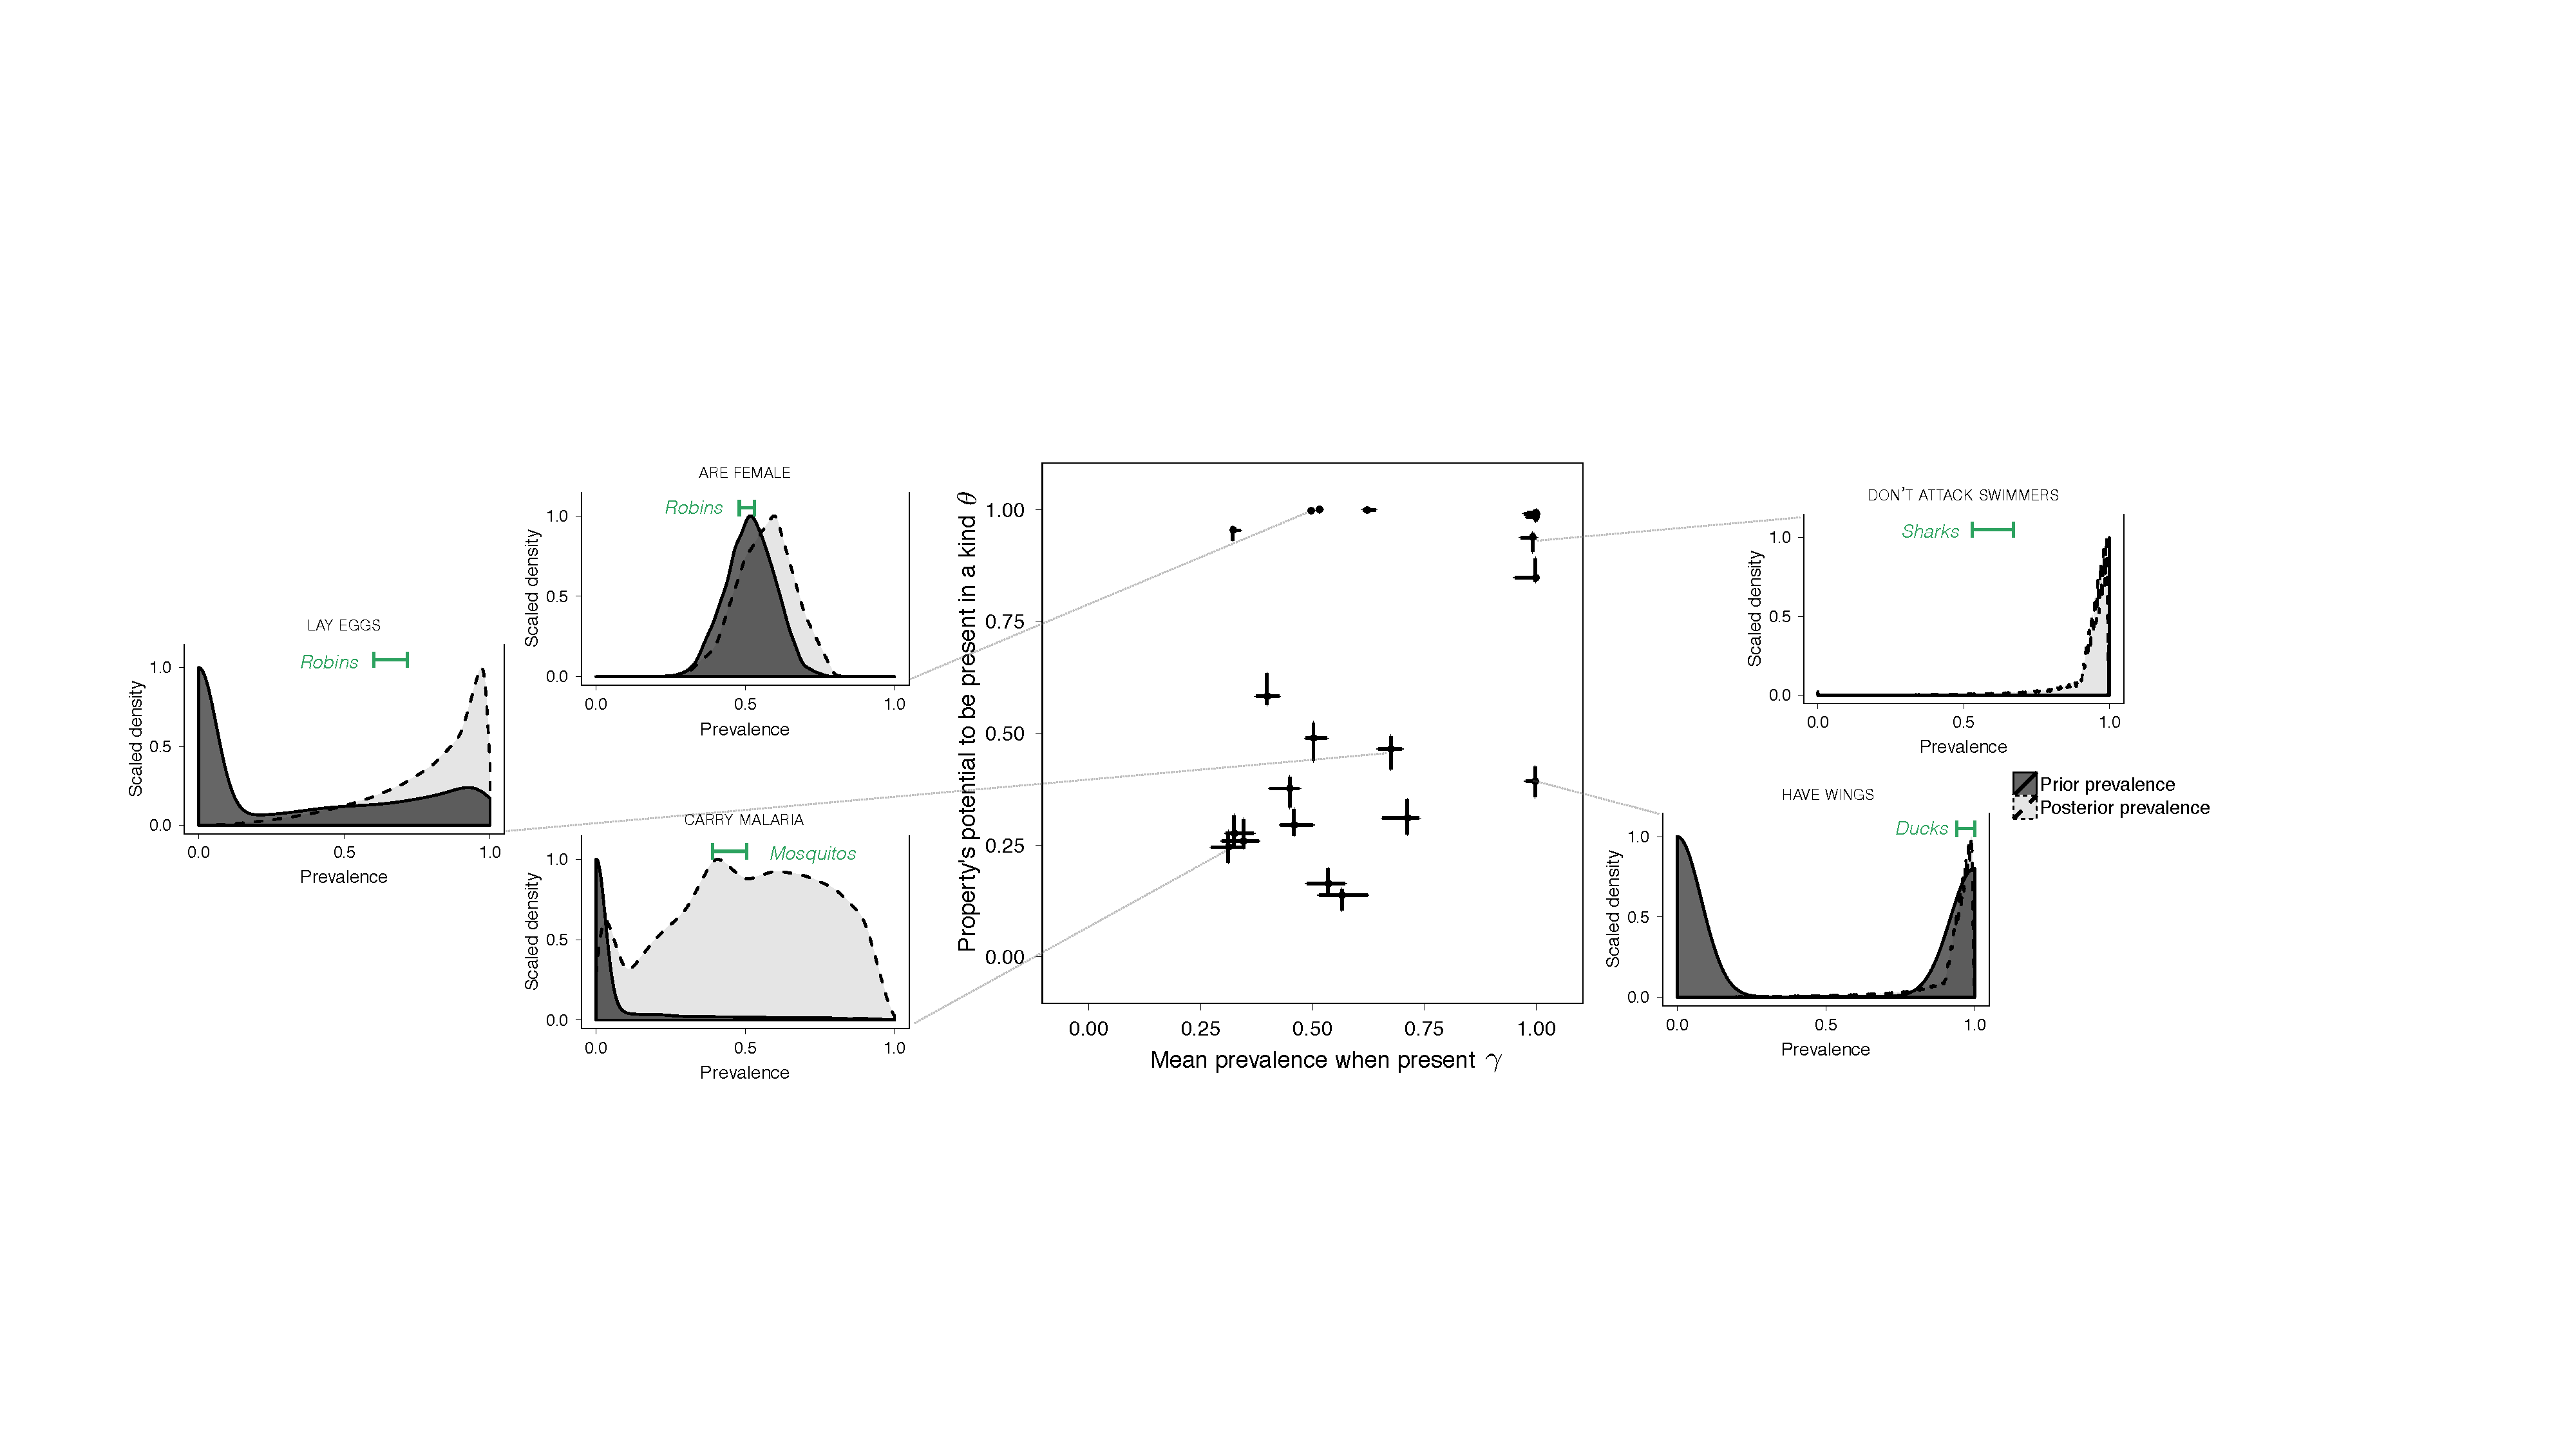
\includegraphics[width=\columnwidth]{prevalence-scatter-wDists_wide.pdf}
    \caption{Prevalence prior distributions empirically elicited for twenty-one animal properties.
    Prior distributions are summarized by $\theta$----a property's potential to be present in a category----and $\gamma$----the mean prevalence when it is possible for the property to be present in a category.
    Inset plots display example empirical prior distributions over prevalence together with corresponding $L_1$ model predictions: the posterior after hearing a generic utterance. 
    Intervals on the top of plots show human beliefs about the prevalence of the property within a target category.
%    Posterior distributions show what happens to a listener's belief about the prevalence after hearing the associated generic. 
    Felicitous generic utterances result when the target prevalence is more likely under the posterior than under the prior.
 %   \ndg{should mark the observed within-category prevalence for target kinds in pop-outs? or maybe one of the axes of main plot should be that?}
     Error bars denote 95\% Bayesian credible intervals (same for Figure \ref{fig:prior2}).
    }
  \label{fig:priors1a}
\end{figure*}




\section*{Experiment 1b: Truth judgments of familiar generics}


We tested the degree to which the $S_2$ model, Eq.~\ref{eq:S2}, coupled with the empirically-elicited $P(x)$ from Expt.~1a predicted that a given category--property pair (e.g. \textsc{robins} and \textsc{lays eggs}) would result in a felicitous generic (e.g. \emph{Robins lay eggs.}). 


\subsection*{Method}

\subsubsection*{Participants}

We recruited 100 participants over MTurk. 

\subsubsection*{Procedure and materials}

Participants were shown thirty generic sentences in bare plural form one after another. 
They were asked to press one of two buttons to signify whether they agreed or disagreed with the sentence (see {\it SI Table 2} for complete list and {\it SI Section B} for more details). 

The thirty sentences cover a range of conceptual distinctions described in Expt.~1a and were constructed to elicit the full range of acceptability judgments (``acceptable'', ``unacceptable'', and ``uncertain'') with low-, medium-, and high-prevalence properties (as measured in Expt.~1a).


\subsubsection*{Data--Model analysis and results}
 
 %Does subjective belief about the prevalence of the property within the target kind predict the felicity of a generic utterance?
From the prevalence-prior data (Expt.~1a) we can estimate participants' beliefs about the prevalence of a property for a given kind (e.g.~the percentage of \textsc{robins} that \textsc{lay eggs}; see green intervals on Figure \ref{fig:priors1a} and \emph{SI Table 2}).
% for Maximum A-Posteriori (MAP) estimates and 95\% Bayesian Highest Density Intervals (HDI) over the mean prevalence for each property--category pairing). %We first compare the predictions of Eq.~\ref{eq:S2} to 
As a simple baseline hypothesis, we first explore whether these prevalence values themselves predict generic endorsement (e.g.~does the fraction of \textsc{robins} that \textsc{lay eggs} predict the felicity of \emph{Robins lay eggs}?).
A little over half of the variance in truth judgments data is explained by the prevalence of the property within the kind alone ($r^2 = 0.599$; MSE=0.065; \emph{SI Figure 2}). 
This is not surprising given the existence and our inclusion of high-prevalence true generics (e.g. \emph{Leopards have spots.}) and low-prevalence false generics (e.g. \emph{Leopards have wings.}) in our stimuli. 
However, large deviations from a purely target-category prevalence account remain: Generics in which the target category has intermediate prevalence (prevalence quartiles 2 and 3: $ 20\% < prevalence < 64\%$), are not at all explained by prevalence within those categories ($r_{Q2,3}^2 = 0.029$; MSE = 0.110).

We instead use the measured within--kind prevalence as the subjective probability that speaker $S_2$ in Eq.~\ref{eq:S2} is trying to communicate.
Having inferred likely priors empirically, the model has 1 parameter: the speaker optimality parameter $\lambda$ (in Eq.~\ref{eq:S1}).
We integrate out the likely values of this parameter using Bayesian data analytic techniques \cite{LW2014} (see SI Section B for full details).
The pragmatic speaker model $S_2$, using empirically measured priors, does a much better job of explaining the truth judgments ($r^2=0.981$; MSE=0.003; Figure \ref{fig:modeldataBars}, {\it SI Figure 4}). 
Generics that received definitive agreement or disagreement are predicted to be judged as such by the model (corners of Figure \ref{fig:modeldataBars}), including items for which target-category prevalence is not a good indicator of the acceptability (for prevalence quartiles 2 and 3, $r_{Q2,3}^2=0.955$; MSE=0.005; Figure \ref{fig:modeldataBars}, intermediate shades).
The probabilistic pragmatics model explains the puzzling flexibility of generic truth-conditions as the result of communicative pressures (\emph{be truthful}, \emph{be informative}) operating over diverse prior beliefs about the properties. 
 


%\begin{figure}
%\centering
%    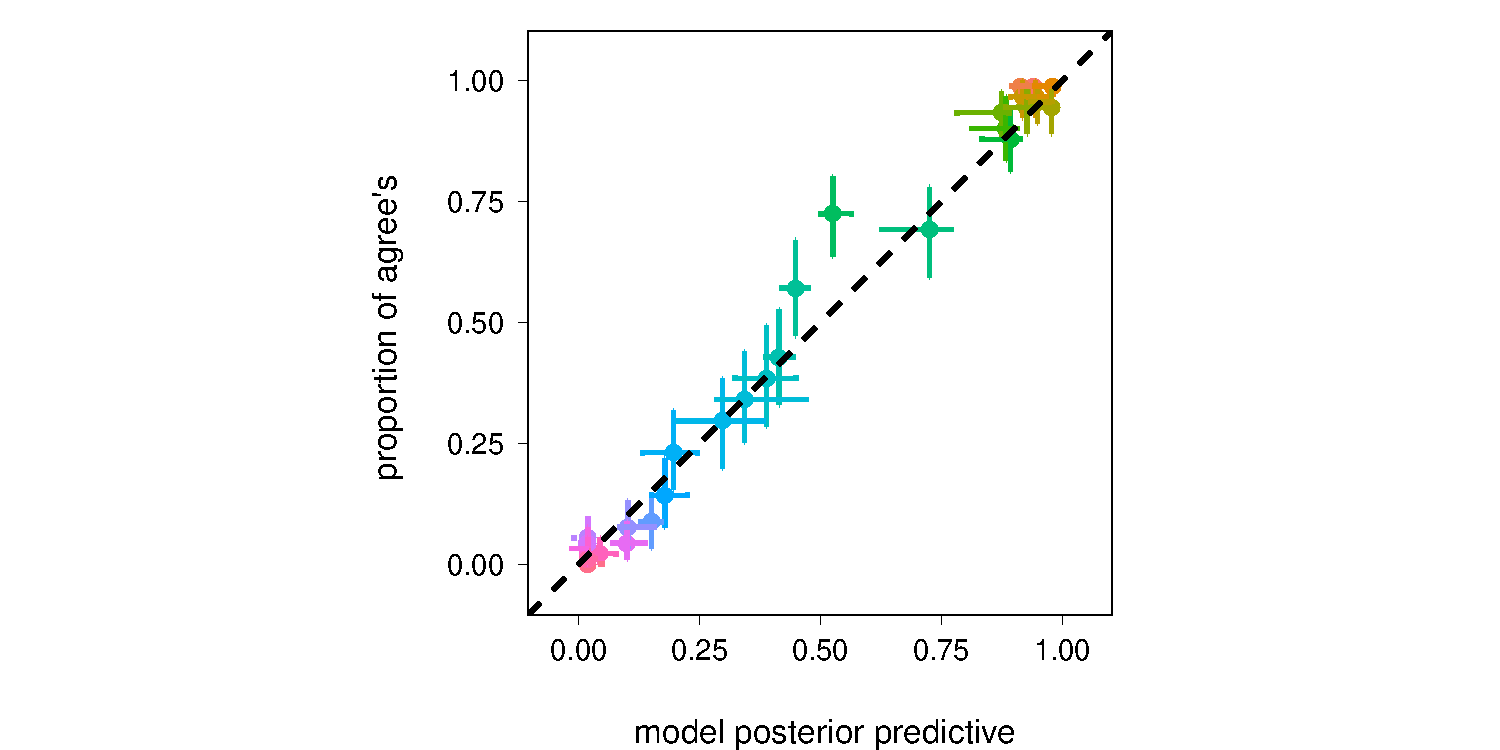
\includegraphics[width=\columnwidth]{tj_n100_tjVsPostpred_95hdi.pdf}
%    \caption{Truth judgments from Expt.~1b for each item vs. the posterior predictive MAP estimates for the target item using the lifted-threshold model with the empirical priors elicited in Expt.~1a. Color spectrum corresponds to the rank ordering of the truth judgment data; similarly colored dots received similar truth judgments. Error bars correspond with 95\% bootstrapped confidence intervals for the participant data and 95\% highest probability intervals for the model predictions.}
%  \label{fig:modeldataScatter}
%\end{figure}


%Participants were restricted to those with US IP addresses and with at least a 95\% MTurk work approval rating. 
%4 participants were excluded for failing to pass a catch trial.
%5 participants self-reported a native language other than English; removing their data has no effect on the results reported. 
%The experiment took about 3 minutes and participants were compensated \$0.35.
%Participants were asked to report whether they agreed or disagreed with generic sentences presented in bare plural form. 
%Items were presented sequentially, and participants reported whether or not they agreed with the sentence by pressing either \textsc{p} or \textsc{q} (randomized between-subjects). 
%Generic sentences were selected to correspond with the properties used in Expt.~1a. 
%Approximately 10 true, 10 false, and 10 uncertain truth-value generics were selected (see {\it SI Table 2} for full list of items).
%As a manipulation check, participants were asked at the end of the trials which button corresponded to ``Agree''. 
%4 participants were excluded for failing this trial.
%

%\ndg{maybe one more sentence about the desired range of variation: from true to false and in between, but also true with low prevalence, etc...?}
%
%The 30 generic sentences fell into 3 \emph{a priori} categories: definitely true, definitely false, and neither true nor false (Figure \ref{fig:modeldataBars}, light bars). 

%%the manipulation check here doesn't add much... moved to supplement...
%As a manipulation check, the \emph{a priori} truth-judgment we assigned was a significant predictor of the empirical truth judgments: true generics were significantly more likely to be agreed with than the indeterminate generics ($\beta = 3.14; SE = 0.15; z = 21.5$), as revealed by a mixed-effect logistic regression with random by-participant effects of intercept.
%Indeterminate generics were agreed with \emph{less} likely than chance ($\beta = -0.49; SE = 0.09; z = -5.3$) but significantly more than false generics ($\beta = 2.09; SE = 0.14; z = 14.5$).


%The probabilisitic model of generic production is fully specified by Eqs.~\ref{eq:L1} -- \ref{eq:S2}, the empirically-elicited $P(x)$, and the speaker rationality parameter $\lambda$ in Eq.~\ref{eq:S1}. 
%Because $\lambda$ is not of theoretical interest here, it is marginalized according to Bayesian data analysis principles \cite{LW2014}. 
% $P(x)$ describes the belief distribution on the prevalence of a given property (e.g. \textsc{lay eggs}) across relevant categories. 
% This distribution, which is conceivably very different for different properties, is common-sense background knowledge. 
% We measure it empirically by asking participants ($n=57$) about the prevalence of our target properties for many different animal categories\footnote{Our experiments stay within the animal kingdom because we expect there to be considerably less variability in participants beliefs about animals than about other types of categories (e.g. social categories)}. 
% 
%, which is crucial since this drives variance in model predictions.


%for four example properties---there are substantial differences between different types of properties. 
%\ndg{how about being more specific about what we mean by between and within category (mass on zero; mean of remaining mass?). say the model suggests these are important. make a plot showing these for all our properties..?}

%The property ``lays eggs'' is relatively rare across categories (large density at 0); even when some animals within a category have manes, there is considerable variation of the percent that do, though the expected value is around 67\% (Figure \ref{fig:priors1a} bottom left; within-category prevalence given by blue dotted line). 
%By contrast, the distribution over ``is male'' has a lot less diffuse: the property is highly prevalent across categories (almost no mass at 0), and within a category it is present in about 50\% of cases.
%The property ``has wings'' is not particularly rare across categories (probably owing to the fact that bird categories are heavily represented in our stimulus set), and within a category is widespread, as reflected by the bimodal distribution. 
%Finally, ``has malaria'' is an example of a property that is both rare across-categories and within-categories. 
%The property is absent from most animal species, and even when it is present, it is only present in a small number of cases.





%\begin{figure*}
%\centering
%\begin{minipage}[b]{.49\textwidth}
%    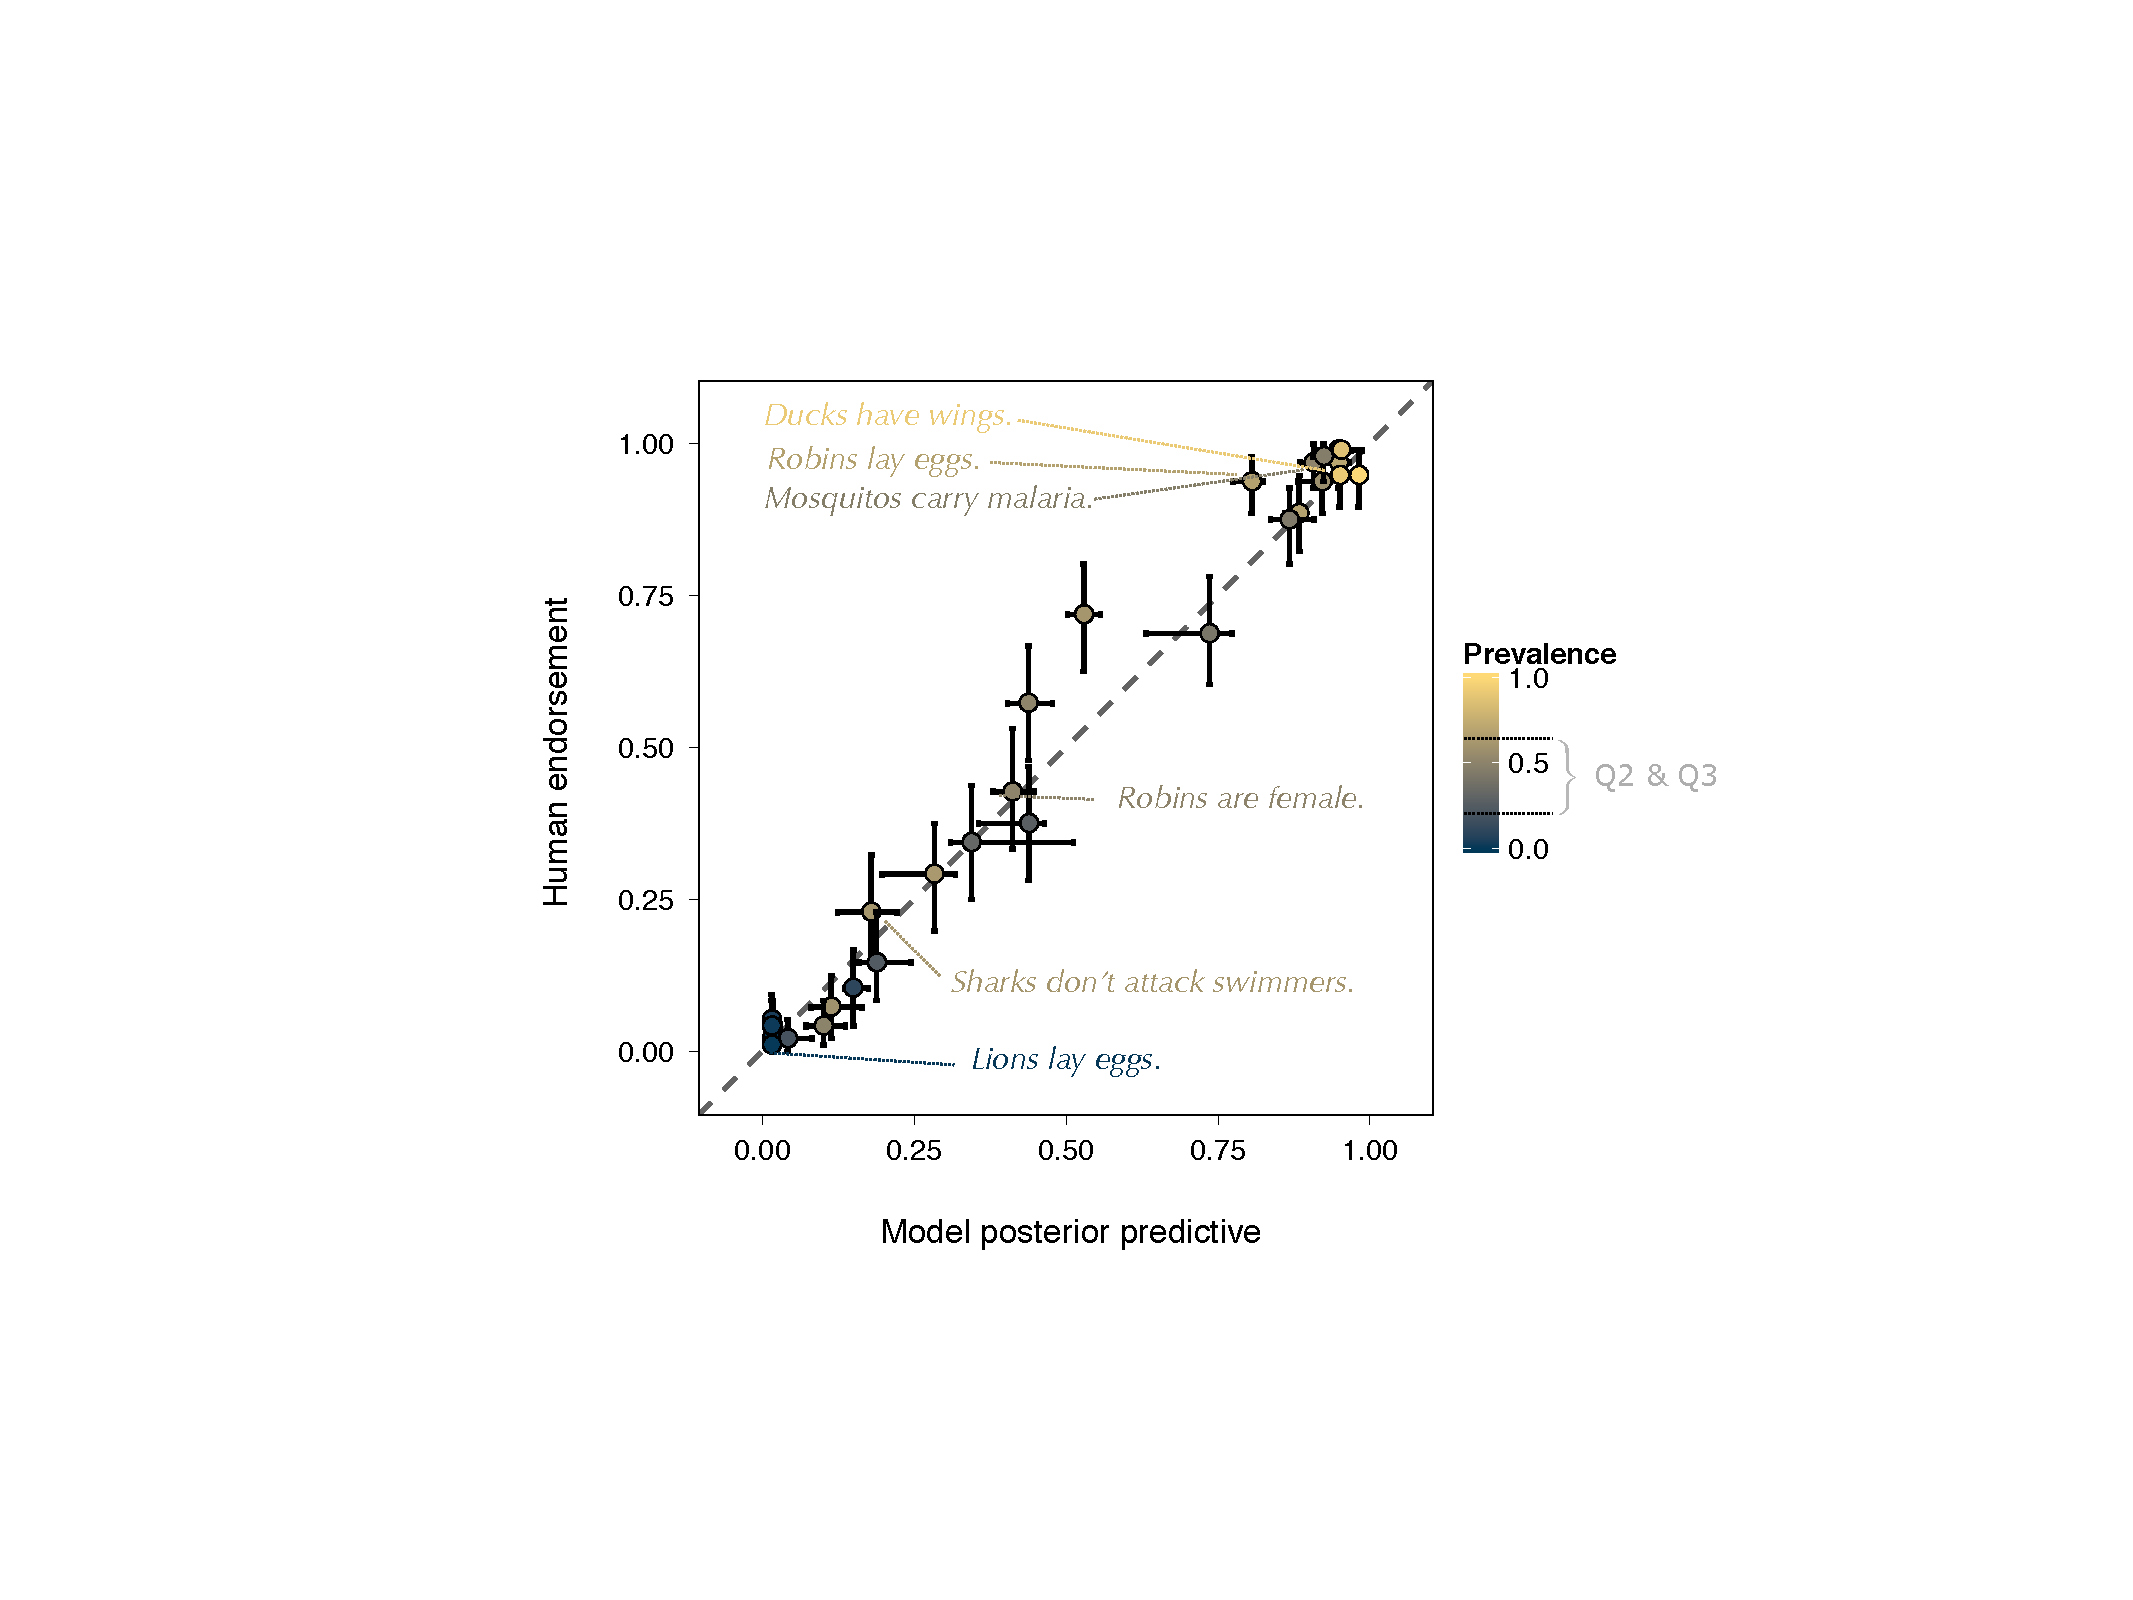
\includegraphics[width=8.7cm]{truthjudge-scatter-wLabels.pdf}
%    \caption{Human acceptability judgments and model predictions for thirty generic utterances about familiar animals and properties. 
%    Color denotes target-category prevalence of the property, with darker colors indicating lower prevalence. 
%    Intermediate prevalences (quartiles 2 \& 3) are in intermediate shades (marked on color bar).
%    Error bars correspond with 95\% bootstrapped confidence intervals for the participant data and 95\% highest probability intervals for the model predictions.
%    }
%  %\label{fig:modeldataBars}
%\end{minipage}
%\begin{minipage}[b]{.49\textwidth}
%\centering
%    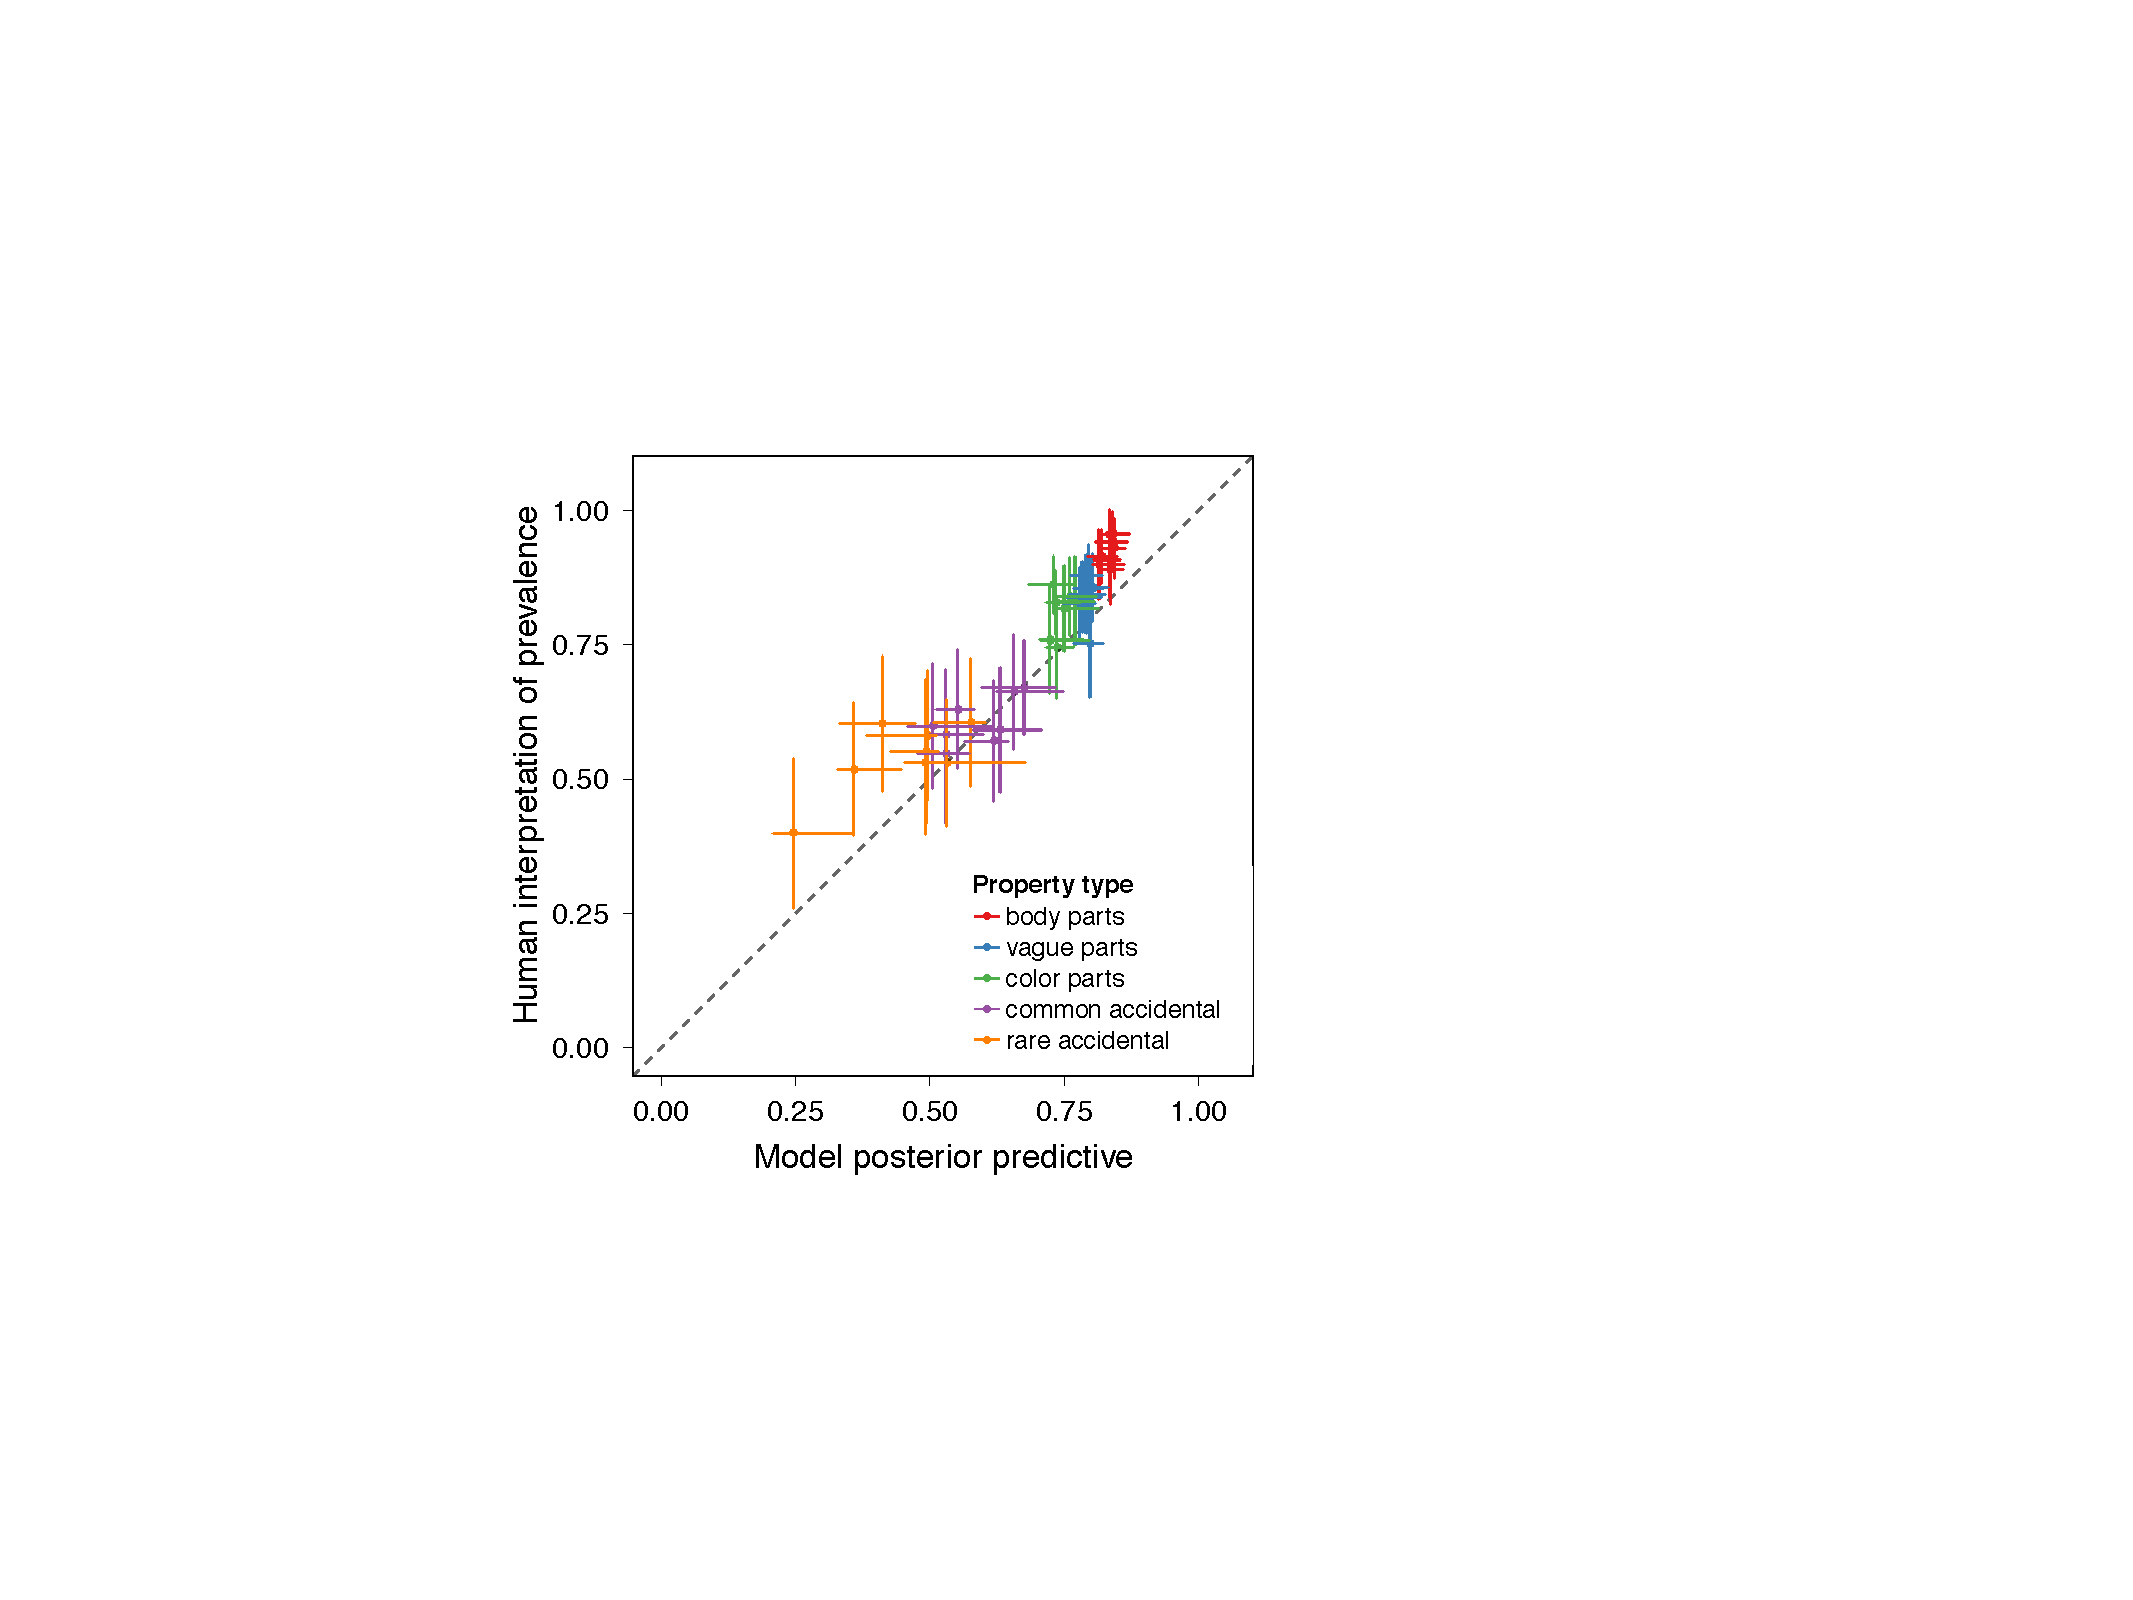
\includegraphics[width=6.7cm]{implied-byItem-mh100kX2b.pdf}
%    \caption{Human interpretation of prevalence upon hearing a generic compared with the $L_1$ model posterior predictive. 
%    Participants display graded endorsements of generics in terms of prevalence based on type of property (which is also associated with \emph{mean prevalence when present} $\gamma$, see Figure 3).
%    The model displays the same variability of interpretation, producing strong interpretations for generics of biological properties (red, blue, green) and weaker interpretations of generics of accidental properties (purple, orange).
%        Error bars denote bootstrapped 95\% confidence intervals for the data and Bayesian 95\% credible intervals for the model.}
% % \label{fig:impliedByItem}
%\end{minipage}
%\end{figure*}

\begin{figure}
\centering
    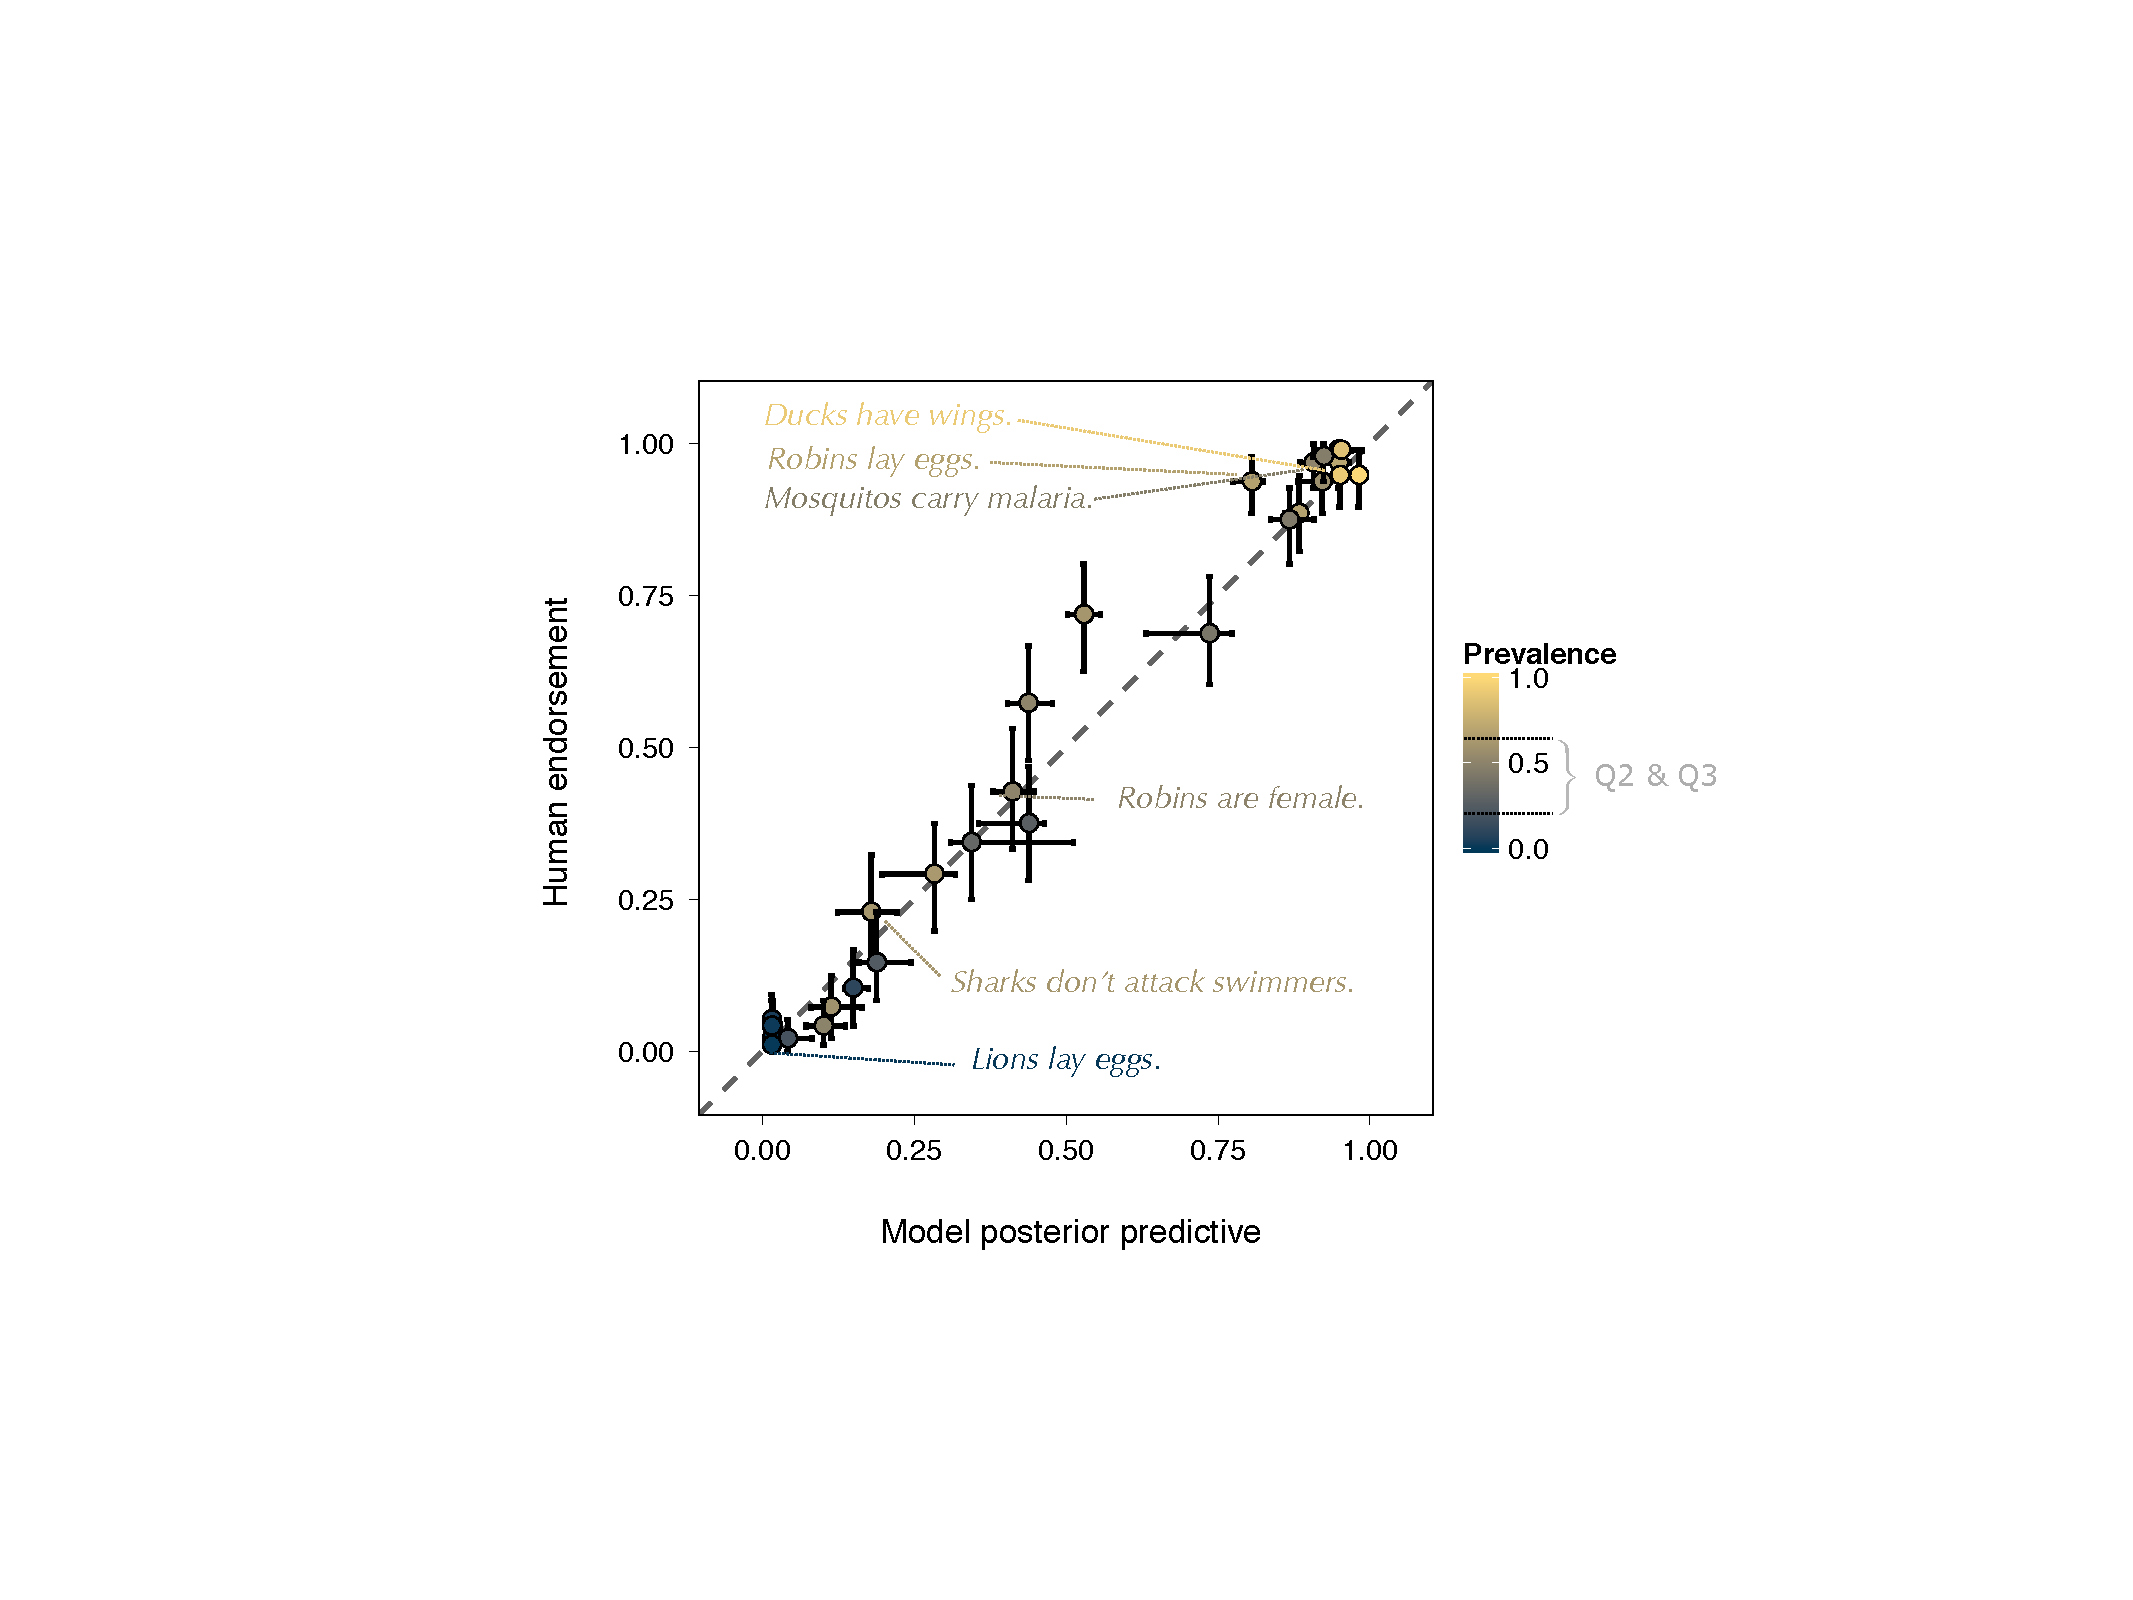
\includegraphics[width=0.7\columnwidth]{truthjudge-scatter-wLabels.pdf}
    \caption{Human acceptability judgments and model predictions for thirty generic utterances about familiar animals and properties. 
    Color denotes target-category prevalence of the property, with darker colors indicating lower prevalence. 
    Intermediate prevalences (quartiles 2 \& 3) are in intermediate shades (marked on color bar).
    Error bars correspond with 95\% bootstrapped confidence intervals for the participant data and 95\% highest probability intervals for the model predictions (same for Figures \ref{fig:impliedByItem} and \ref{fig:exp2b}).
    }
  \label{fig:modeldataBars}
%\end{minipage}
%\begin{minipage}[b]{.49\textwidth}
%\centering
%    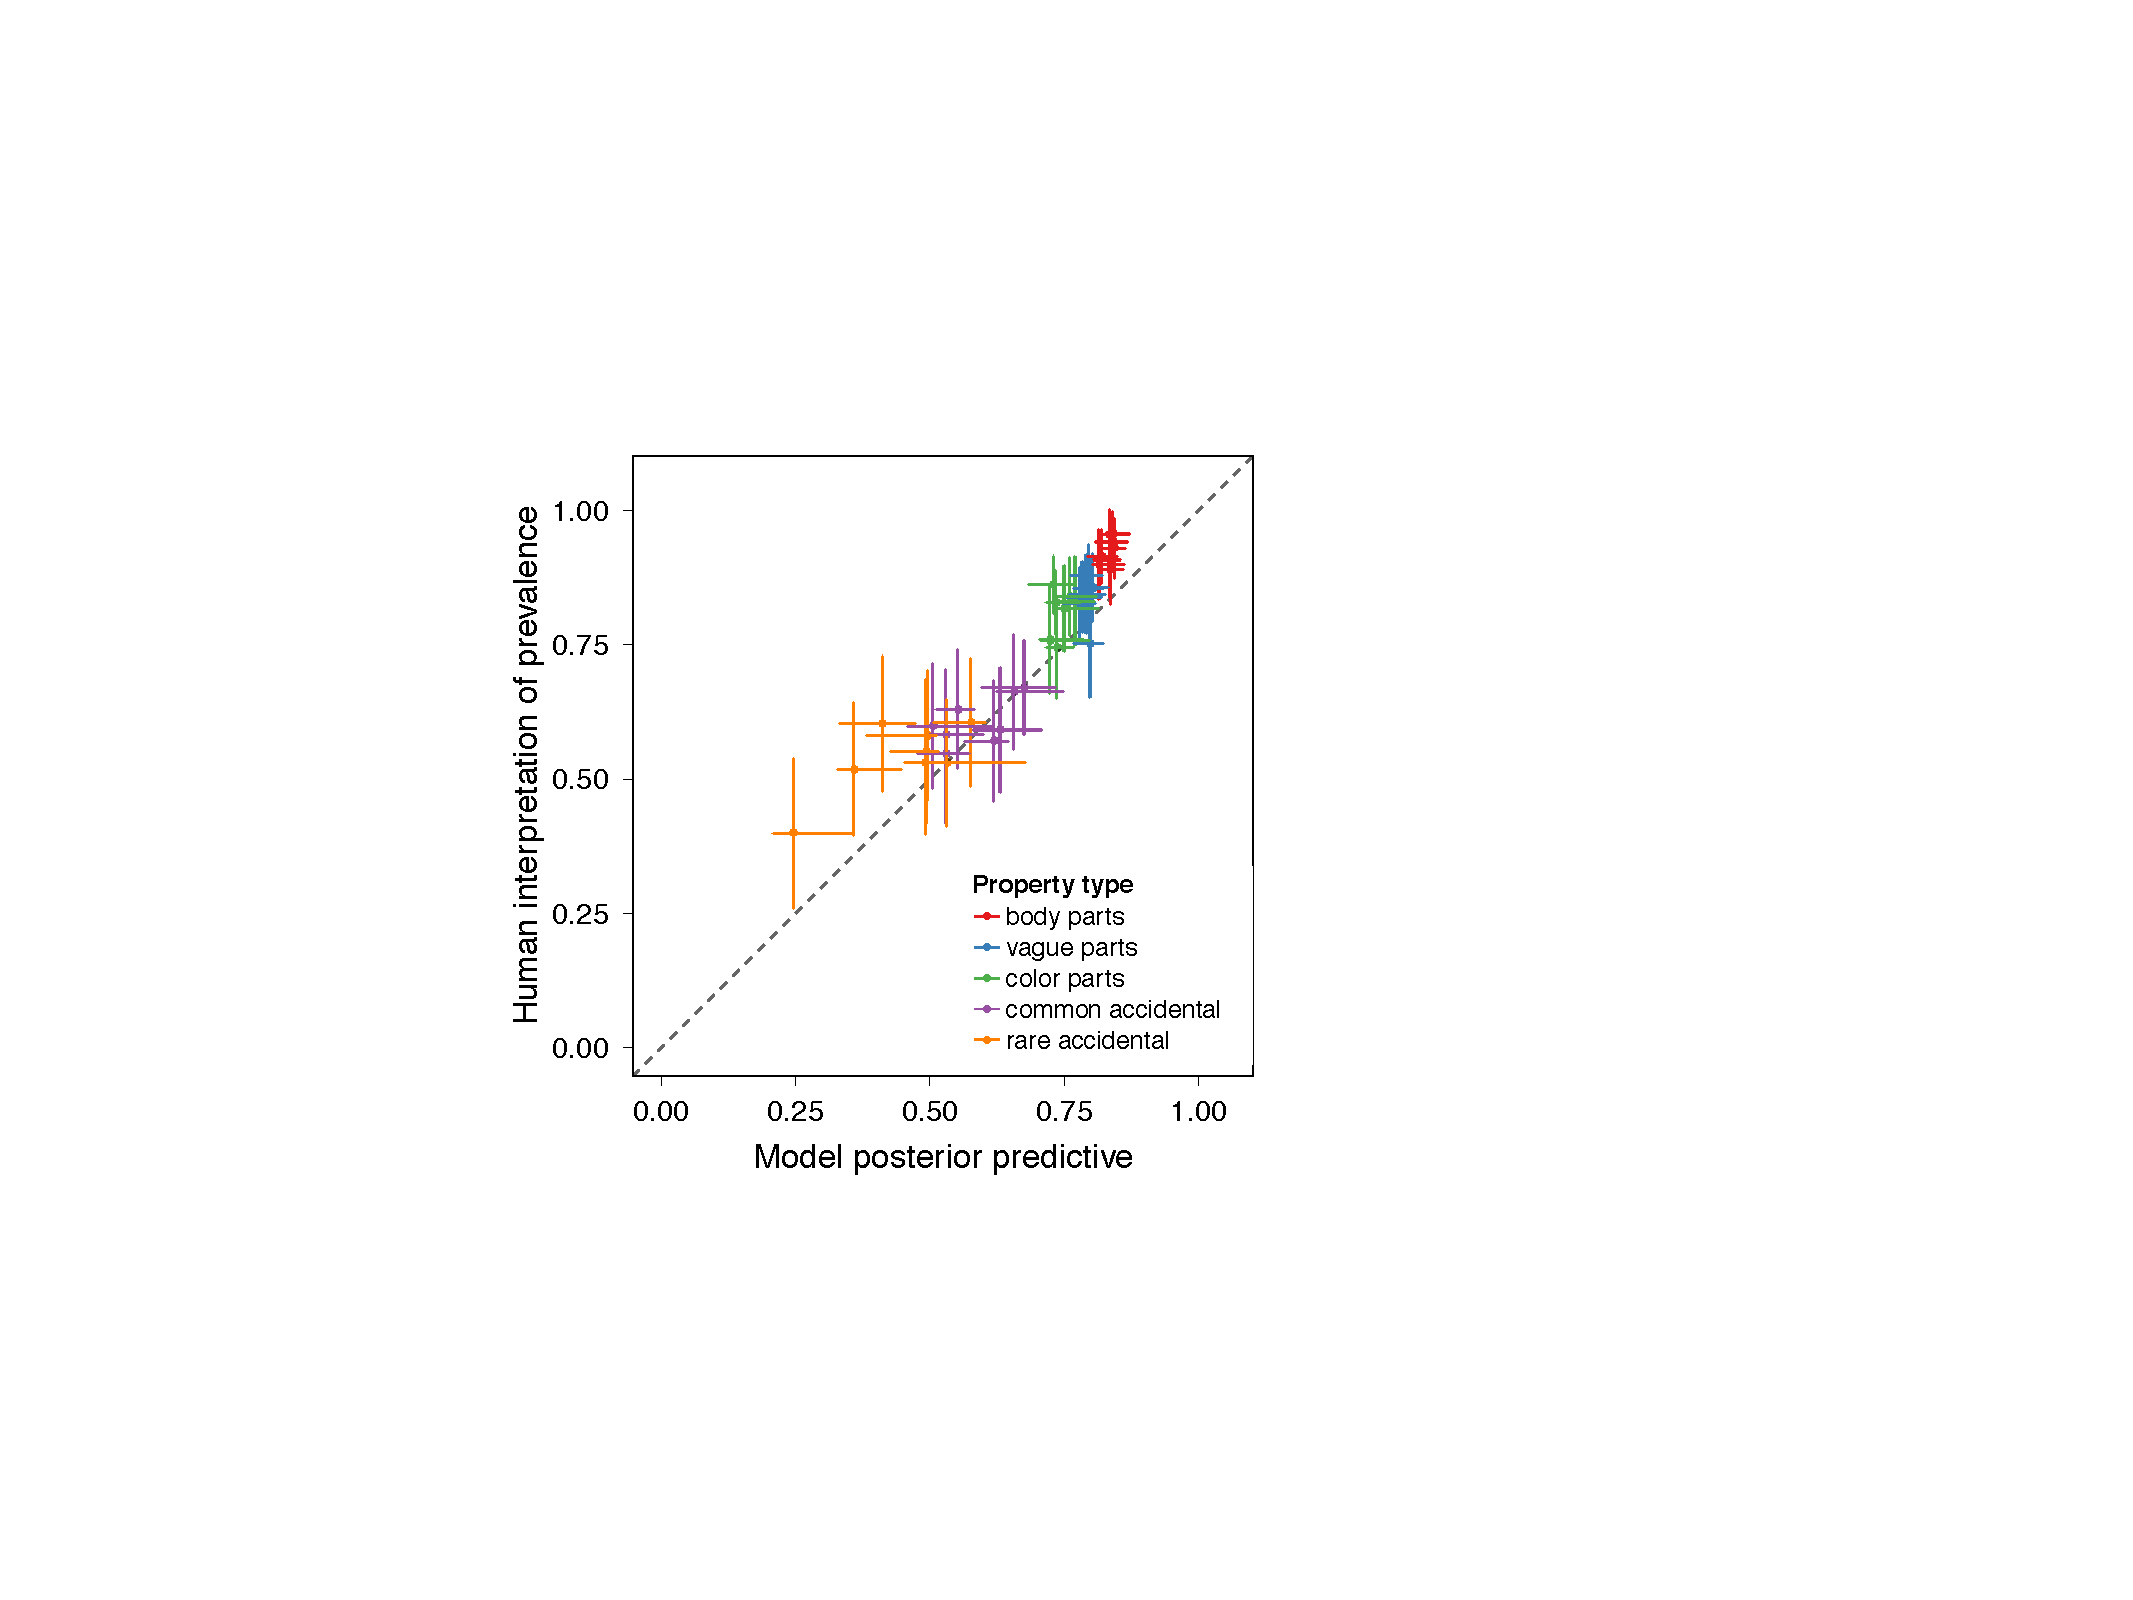
\includegraphics[width=6.7cm]{implied-byItem-mh100kX2b.pdf}
%    \caption{Human interpretation of prevalence upon hearing a generic compared with the $L_1$ model posterior predictive. 
%    Participants display graded endorsements of generics in terms of prevalence based on type of property (which is also associated with \emph{mean prevalence when present} $\gamma$, see Figure 3).
%    The model displays the same variability of interpretation, producing strong interpretations for generics of biological properties (red, blue, green) and weaker interpretations of generics of accidental properties (purple, orange).
%        Error bars denote bootstrapped 95\% confidence intervals for the data and Bayesian 95\% credible intervals for the model.}
% % \label{fig:impliedByItem}
%\end{minipage}
\end{figure}


\section*{Empirical puzzle 2: Generics have strong interpretations}
Perhaps the most important role for generic language is to provide information about new or poorly understood categories. 
To study this we must look to \emph{interpretation} of novel generics (e.g. \cite{Gelman2002, Cimpian2010}).
The pragmatic listener model (Eq.~\ref{eq:L1}) describes interpretation of a generic utterance, without previous knowledge of how common the property is within the target-kind. 
With an uncertain meaning and the pressure to be informative, interpretation is heavily driven by \emph{a priori} beliefs about properties. 
Classic work in generalization suggests beliefs about the prevalence of properties differ by type of property, including relatively fine distinctions between properties that are all biological in nature \cite{Nisbett1983}. 



We used forty different properties to explore a wide range of \emph{a priori} beliefs about prevalence. 
These items make up five categories of properties: biological parts (e.g. \textsc{has claws}), color adjectives about parts (e.g. \textsc{has green feathers}), vague adjectives about parts (e.g. \textsc{has small wings}),  common accidental or disease states (e.g. \textsc{has wet fur}) and rare accidental or disease states (e.g. \textsc{has swollen ears})\footnote{The distinction between common and rare accidental properties was determined empirically by analyzing the data by item, and performing a median split based on the \emph{a priori} mean prevalence when present, $\gamma$, of the property.}.
$P(x)$ was measured empirically ($n=40$, {\it Experiment 2a}), and the most likely priors were inferred using the same structured, statistical approach used for the familiar generics experiment.


\begin{figure*}
\centering
    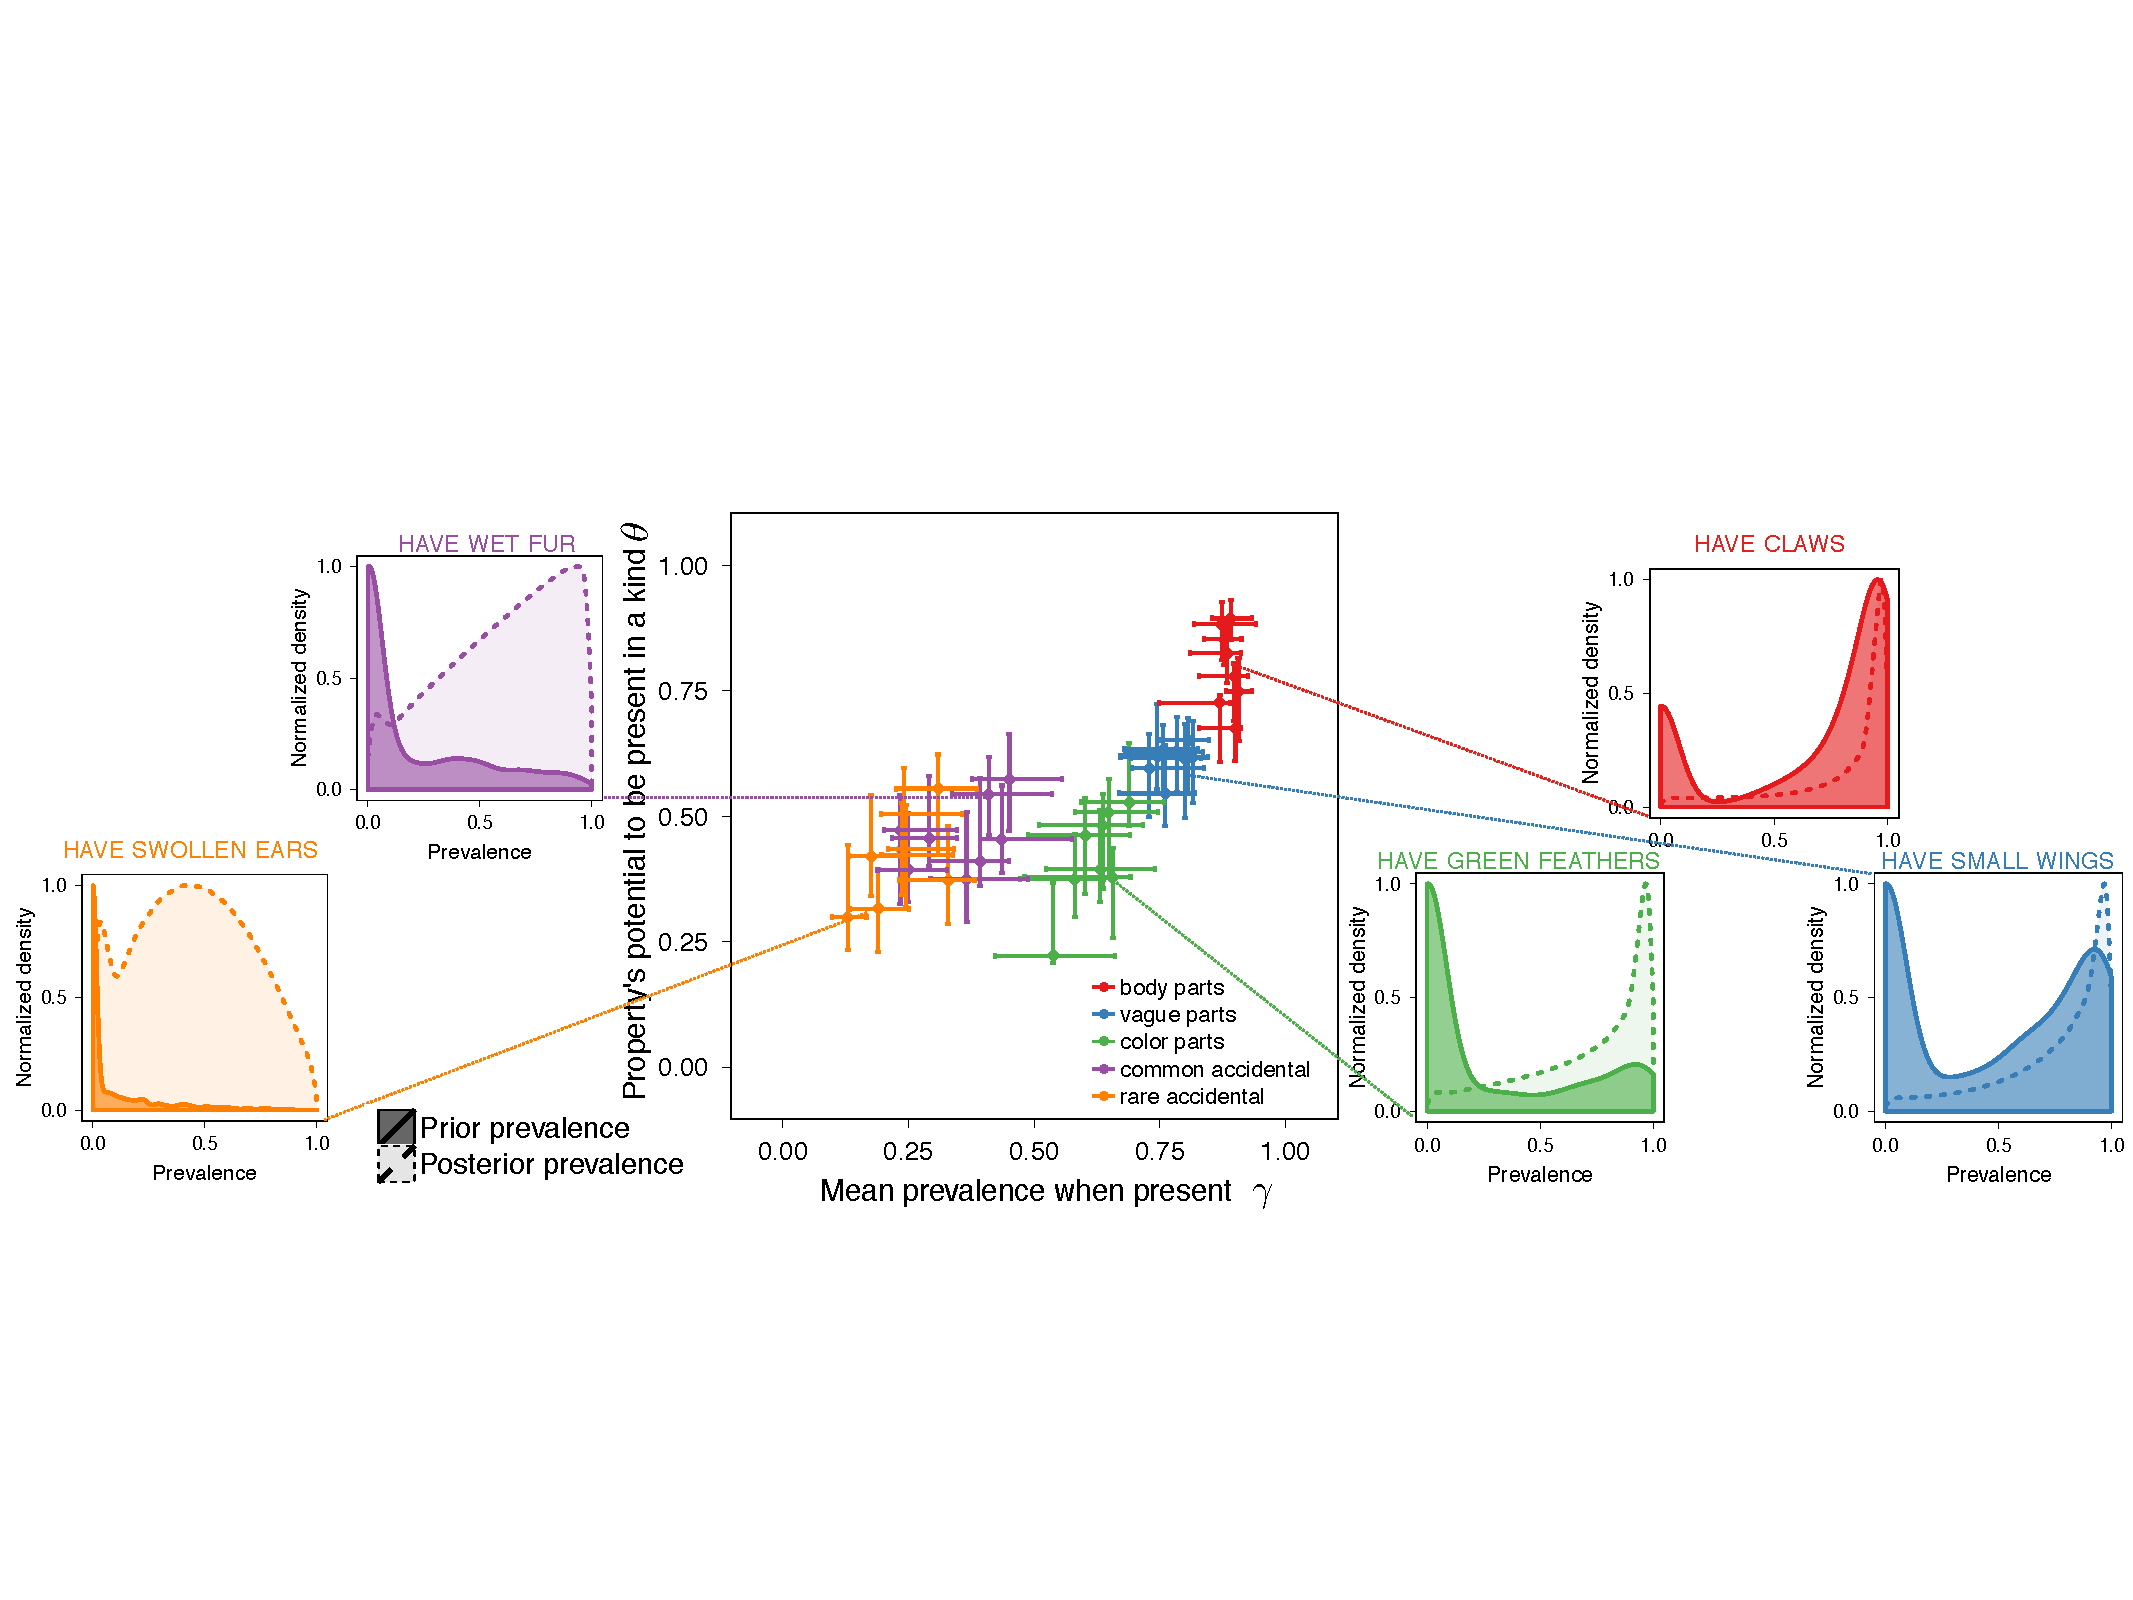
\includegraphics[width=\columnwidth]{prevalence-asymmetry-scatterwDists-byItem3.pdf}
    \caption{Prevalence prior distributions empirically elicited for 40 animal properties.
    Parameters of the structured statistical model---$\theta$ and $\gamma$---reveal quantitative differences in beliefs about the prevalence of conceptually different types of properties (scatterplot). 
    Inset plots show differences in shapes between biological properties (red, green, blue; bimodal) and accidental properties (orange, purple; unimodal).   
  These differences give rise to the variability of interpretations of generic utterances. 
  %    Error bars denote Bayesian 95\% credible intervals.
  }
  \label{fig:prior2}
\end{figure*}


Biological properties are expected to be \emph{a priori} more prevalent (when present) than accidental properties, with fine-grained differences even among types of biological and accidental properties (Figure \ref{fig:prior2}).
%Interpretations of generic language are readily explored in our model of a listener (Eq.~\ref{eq:L1}), who hears a generic and is trying to infer how widespread the property is. 
The shapes of the prevalence distributions for different properties are importantly diverse (insets). 
Biological properties (``biological'', ``vague'', ``color'' body parts) are bimodal with peaks at 0\% and near-100\% prevalence. 
After hearing the generic, the listener ($L_1$ model, Eq.~\ref{eq:L1}) updates this distribution to a concave posterior peaked at 100\% (Figure \ref{fig:prior2}; red, blue and green insets). 
Accidental properties (``rare'' and ``common'') follow unimodal prior distributions and update to convex posterior distributions, reflecting a higher degree of residual uncertainty after hearing the generic utterance as compared to the biological properties. 

%) 


%Since we are exploring how beliefs are \emph{updated} by generic language, we use novel animal categories (e.g. \textsc{lorches}) in our experiment, following 
%\cite{Cimpian2010}.
%We test experimentally how beliefs are updated by generic language using novel animal categories 
%by using novel animal categories and properties (e.g. \emph{Lorches} and \emph{have green feathers}) to explore how generic language updates one's beliefs. 
%It is strange to measure participants' beliefs about these novel category---property pairs directly (e.g. answering ``How many lorches have purple feathers?'', without knowing what a lorch is).
%Instead, we took advantage of the latent structure in the prior elicitation task (Expt.~1a) to ask participants ($n=40$) about the prevalence of a property (e.g. ``has purple feathers'') across-categories (e.g. ``How likely is it that \emph{there is a} lorch that has purple feathers?'') and within-categories (e.g. ``Suppose there is a lorch with purple feathers. What percentage of lorches do you think have purple feathers?''), separately. 
%We used a hierarchical Bayesian approach to reconstruct the prevalence priors of a similar form to Expt.~1a (see Section \ref{sec:bda2} for details).







%The pragmatic listener in Eq.~\ref{eq:L1} is sensitive to the property in question and its corresponding distribution on prevalence.
%type of property (and its corresponding prior distribution on prevalence) when interpreting a novel generic.


We compared the interpretations of the pragmatic listener in Eq.~\ref{eq:L1} to human judgments ($n=40$, {\it Experiment 2b}) about the likely prevalence of the property after hearing a generic about an unfamiliar kind (e.g. \emph{Lorches have green feathers.}). %, in the same spirit as \cite{Gelman2002}. 
Human prevalence judgments after reading the generic were affected by the type of property and its corresponding mean prevalence when present $\gamma$: The more widespread a property is expected to be \emph{a priori}, the stronger the implications of a generic statement ($\beta = 0.57; SE = 0.08; t(39) = 7.12; p < 0.001$)\footnote{These statistics are the result of a mixed-effects linear regression with a maximal mixed-effect structure: Random by-participant effects of intercept and slope}. 
The pragmatic listener model closely aligns with human judgments, displaying the same sensitivity of interpretation to the property information ($r^2(40)=0.89$, MSE=0.006; Figure \ref{fig:impliedByItem}). 
%Particularly, the \emph{a priori} mean conditional prevalence will guide interpretation as it describes the distribution assuming the property is present. \ndg{why?}
%Again, $P(x)$ was measured empirically ($n=40$, see Supplement Section C).
%The five property types fell on a continuum of \emph{a priori} mean conditional prevalence (Figure \ref{fig:prior2}; x-axis). 
%Biological properties are expected \emph{a piori} to be more prevalent within a kind than accidental properties, with fine-grained differences even among types of biological and accidental properties.
%For instance, within a given kind, colored body parts (e.g. \textsc{green wings}) are expected \emph{a priori} to be less prevalent than some gradable adjectives (e.g. \textsc{small wings}). 
%Some accidental properties are expected to be relatively more prevalent \emph{a priori} than others (``common accidental'' vs. ``rare accidental''; e.g. \textsc{wet fur} vs. \textsc{broken legs}; Figure \ref{fig:prior2}, orange and purple plots).

%These distributions are not necessarily peaked at 100\%, and the expected 
%Figure \ref{fig:prior2} (right) shows the region of interest of these distributions by removing the mass at 0. %
%With the exception of the body part category, properties are mostly likely to be absent from the category (Figure \ref{fig:prior2} left; modes of distributions are at 0).
%If the property is present in the category, the most likely prevalence for biological properties (``part'', ``color part'', and ``vague part'') is 100\% (Figure \ref{fig:prior2} right; modes of blue, green, and red distributions are at 1).
%This is not the case with the prevalence priors for accidental properties, for which lower values are more likely (Figure \ref{fig:prior2} right; modes of orange and purples distributions are at some low prevalence).
%\ndg{this analysis has gotten a lot less transparent since i looked last. it's not at all clear why we should care about the gradient against "some". }
%
%However, the generic does more than merely inform a listener that the property is present: 
%A generic carries the communicative force of a speech act, and thus implies the property is \emph{more prevalent} than a listener would expect (Figure \ref{fig:exp2b} solid line lies above $y=x$ line).
%\ndg{i think if we're going to rely on it we need to set this contrast up much more clearly earlier: many properties are never present in most categories. at the least, the generic rules out the absence of the property (ie ``some''). we want to test whether it is stronger than some. -- though really?}
%The listener model (Eq.~\ref{eq:L1}) produced the same strong interpretation along a gradient (Figure \ref{fig:exp2b}, Right, solid line), displaying the sensitivity to abstract beliefs about the properties that human participants show. 
%We performed a by-item analysis comparing the implied prevalence data to model predictions and found a good quantitative fit ($r^2(40) = 0.89$; see Supplement Section D5). 
%\ndg{
%Generics ``once accepted [...] appear to be commonly taken in a rather strong sense, as if the qualifier \emph{always} had implicitly crept into their interpretation'' (\cite{Abelson1966}, Cf.~\cite{Cimpian2010}). 
%\cite{Gelman2002} found that adults interpret novel generic statements about familiar kinds (e.g. \emph{Bears like to eat ants.}) as implying that almost all of the category have the property (e.g. almost all bears like to eat ants).
%Why is generic language interpreted so strongly if the criterion for endorsement is so flexible? 
%}





\subsection*{The asymmetry between truth conditions and interpretations}
%There is a surprising d\'{e}colage between the truth conditions and interpretations of generic language: 
The truth conditions and interpretations of generic language are surprisingly asymmetric: Novel generics are interpreted as implying a higher prevalence than that required to assent to the exact same generic \cite{Cimpian2010}.
% and the average prevalence required to assent to the exact same utterance: generics were interpreted as implying a higher prevalence than required to assent to the same generic.
%\footnote{This asymmetry did not exist for the quantifier ``Most'', thought to be the most similar quantifier to the generic.}.
Our model predicts that this effect should hold, but only for properties with most extreme prior beliefs (particularly mean prevalence when present, $\gamma$; see Figure \ref{fig:exp2b}, right).
To explore this prediction, we recruited participants ($n=40$) to determine the average prevalence at which a speaker would assert a generic ({\it Experiment 2c}). 
%\ndg{why would we want this?} 
We told participants one of five frequencies for each property type (e.g. \emph{50\% of lorches have green feathers.}), and then asked for truth judgments of the corresponding generic sentence (e.g. \emph{Lorches have green feathers.}). 
%which was previously found to be not as sensitive to participants beliefs about the property (but, cf. \cite{Cimpian2010}, Expt.~4).
For both behavioral data and model predictions (Eq.~\ref{eq:S2})  we computed the average prevalence that led to an assenting judgment, for each property type and participant, following the procedure used by \cite{Cimpian2010}.
%We used the same model that we used for the common generics (Eq.~\ref{eq:S2}) to predict this truth judgments task by submitting it to the same averaging analysis as the behavioral data (see Supplement Section D for more details).
%\ndg{the last sentence is totally opaque....} 
%

The speaker $S_2$ model did not make appreciably different predictions as to the average prevalence to accept the generic:
Generics are acceptable for a wide range of prevalence levels for all property types.
%There are no sharp boundaries between acceptable and unacceptable generics. 
A similar absence of a gradient was observed in the human data ($\beta = 2.82; SE = 4.02; t(39) = 0.70; p = 0.49$; Figure \ref{fig:exp2b}, dotted lines). 
Interpretations of generic utterances are stronger than their average truth conditions for biological properties but not for accidental properties (Figure \ref{fig:exp2b}); the extent of the difference is governed by prior property knowledge ($\gamma$, inferred from prior elicitation data).
The listener and speaker pair of models predicts human endorsements and interpretations of novel generic utterances well ($r^2(10) = 0.921$, MSE = 0.004). 


\begin{figure}
\centering
    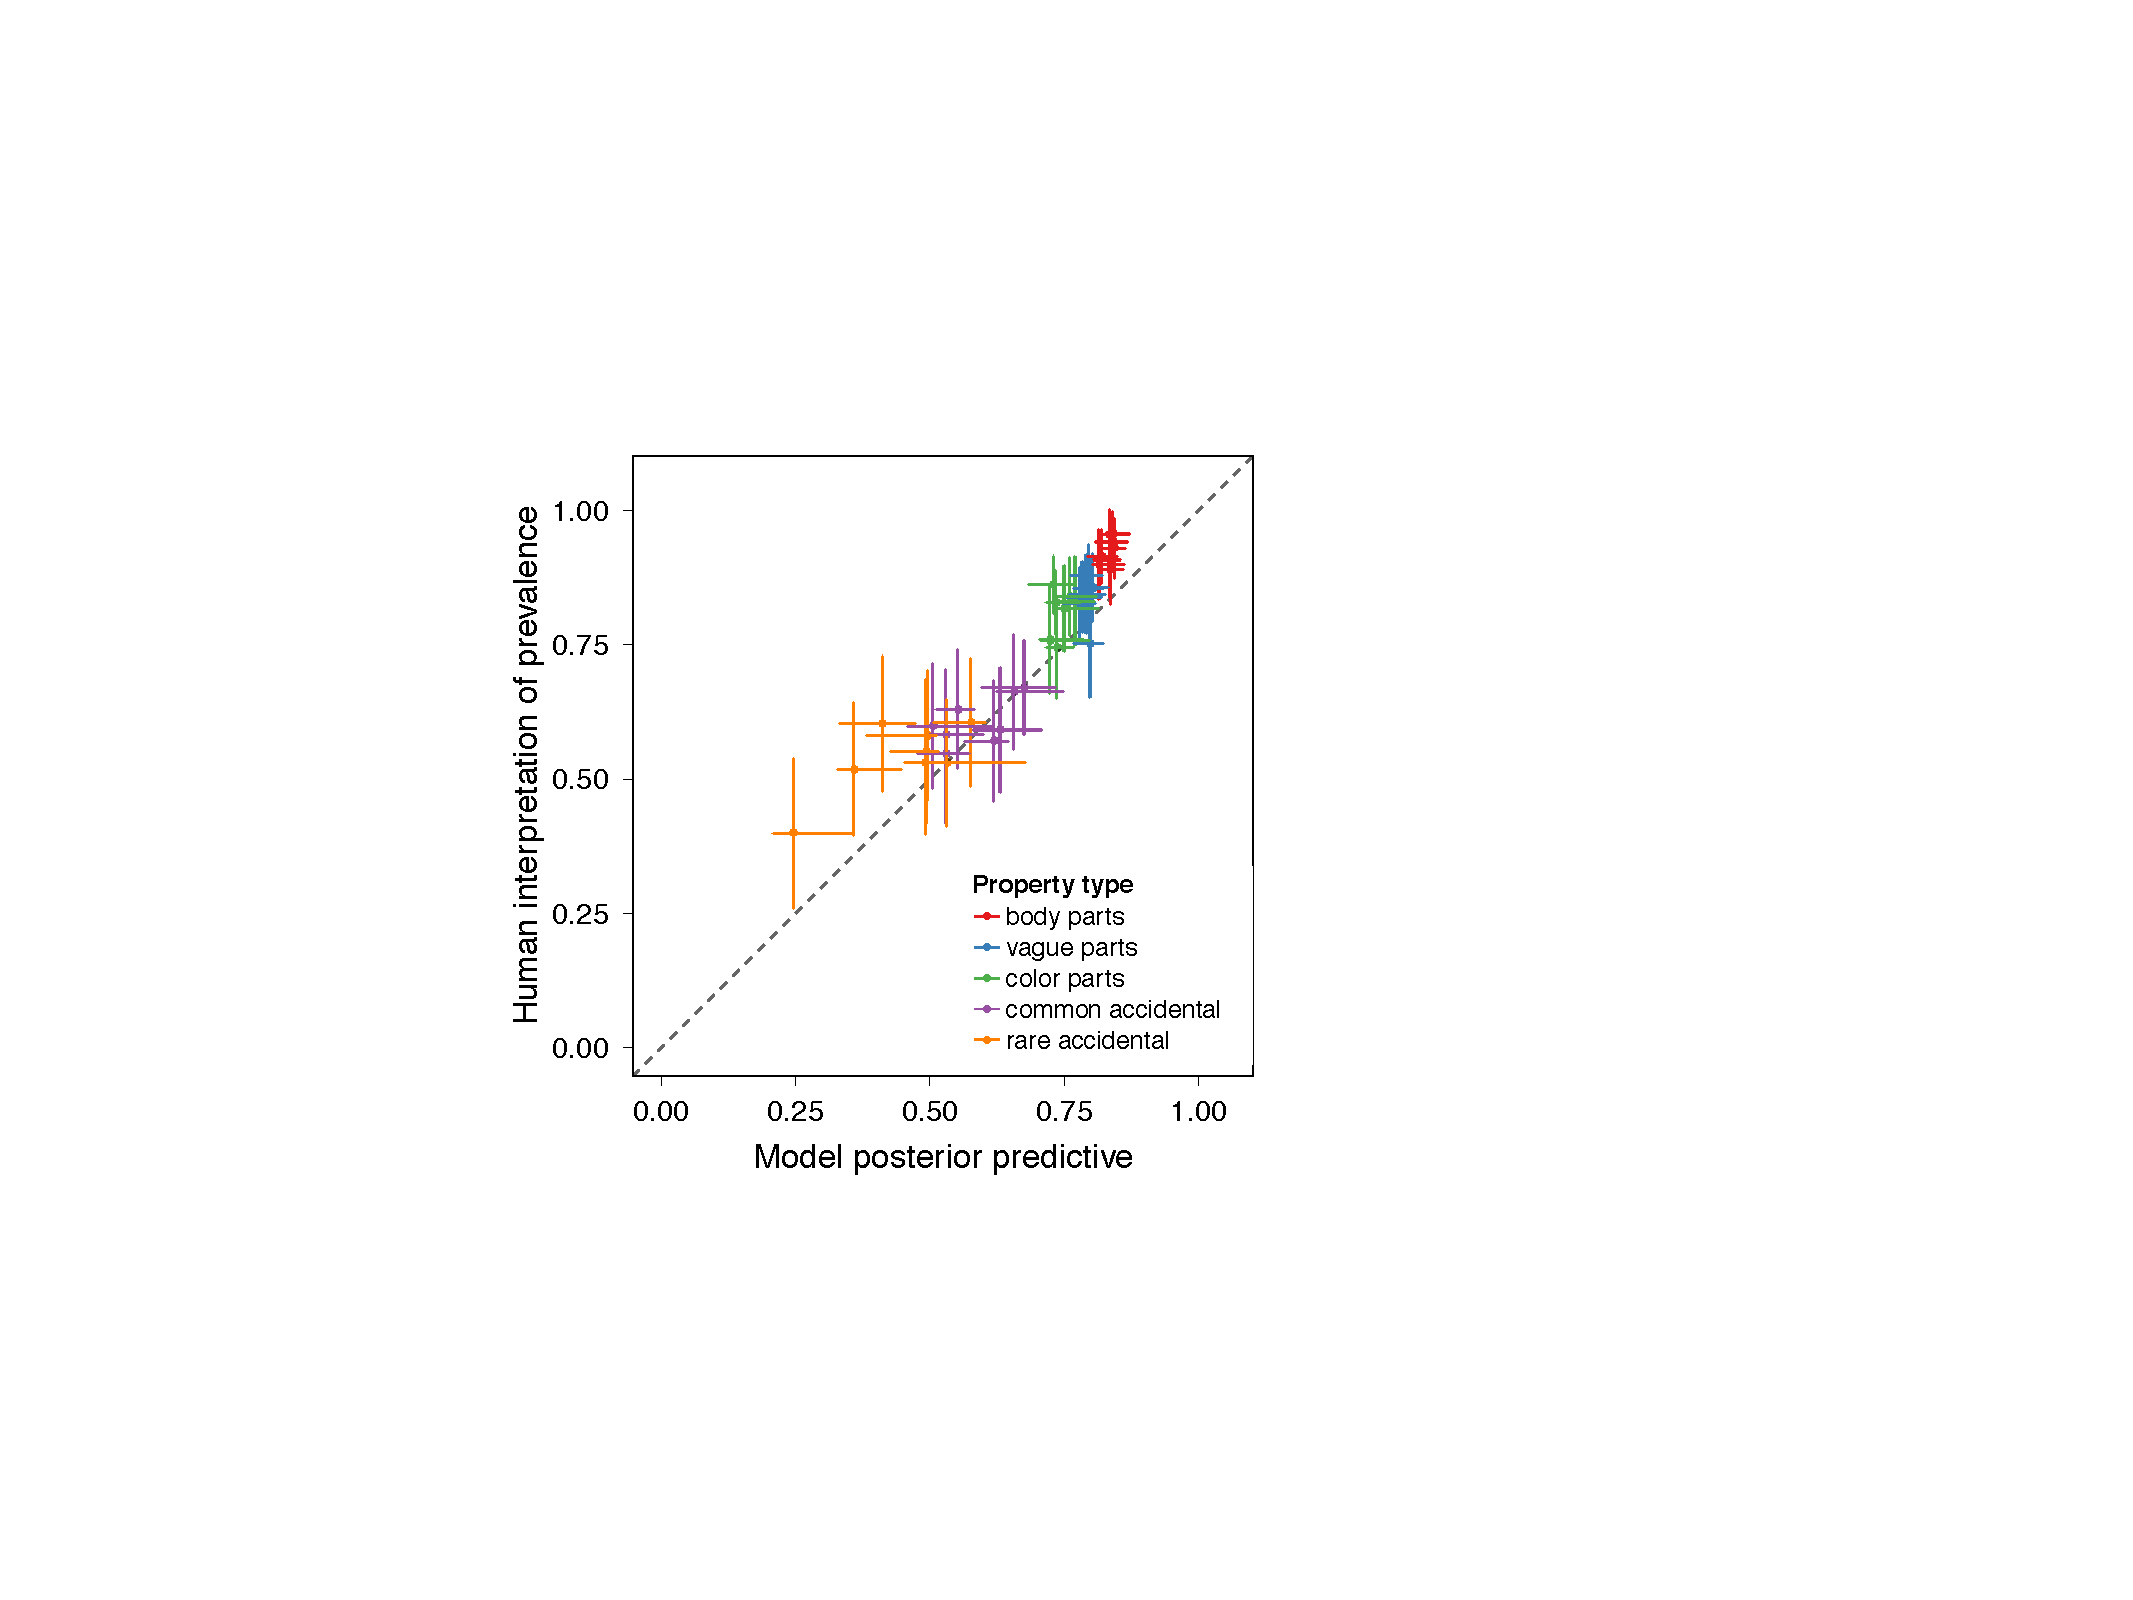
\includegraphics[width=0.7\columnwidth]{implied-byItem-mh100kX2b.pdf}
    \caption{Human interpretation of prevalence upon hearing a generic compared with the $L_1$ model posterior predictive. 
    Participants and the model interpret generics as implying the property is widespread to a degree based on type of property: Generics of biological properties (red, blue, green) have  strong interpretations while generics of accidental properties (purple, orange) are weak.}
    %    Error bars denote bootstrapped 95\% confidence intervals for the data and Bayesian 95\% credible intervals for the model.}
  \label{fig:impliedByItem}
\end{figure}

%Interestingly, we observe greater implied prevalence of common accidental properties than rare accidental properties, given our median split based on the prior elicitation task ($\beta=0.061; SE = 0.025; t(39) = 2.47; p = 0.018$) \footnote{These statistics are the result of a mixed-effects linear regression with a maximal mixed-effect structure: Random by-participant effects of intercept and slope}.
%Implications of generics of body parts was significantly greater than those of the biological properties used by \cite{Cimpian2010} (here, ``color parts'') ($\beta=0.118; SE = 0.024; t(39) = 4.74; p < 0.001$). 
%There was also a trending effect for the implications of vague body parts (e.g. curly fur) to be greater than those of color parts (e.g. yellow fur) ($\beta=0.032; SE = 0.016, t(54.8) = 1.95; p = 0.056$), possibly due to the belief that the same kind of animal can come in many different colors (e.g. dogs).
\begin{figure*}
\centering
    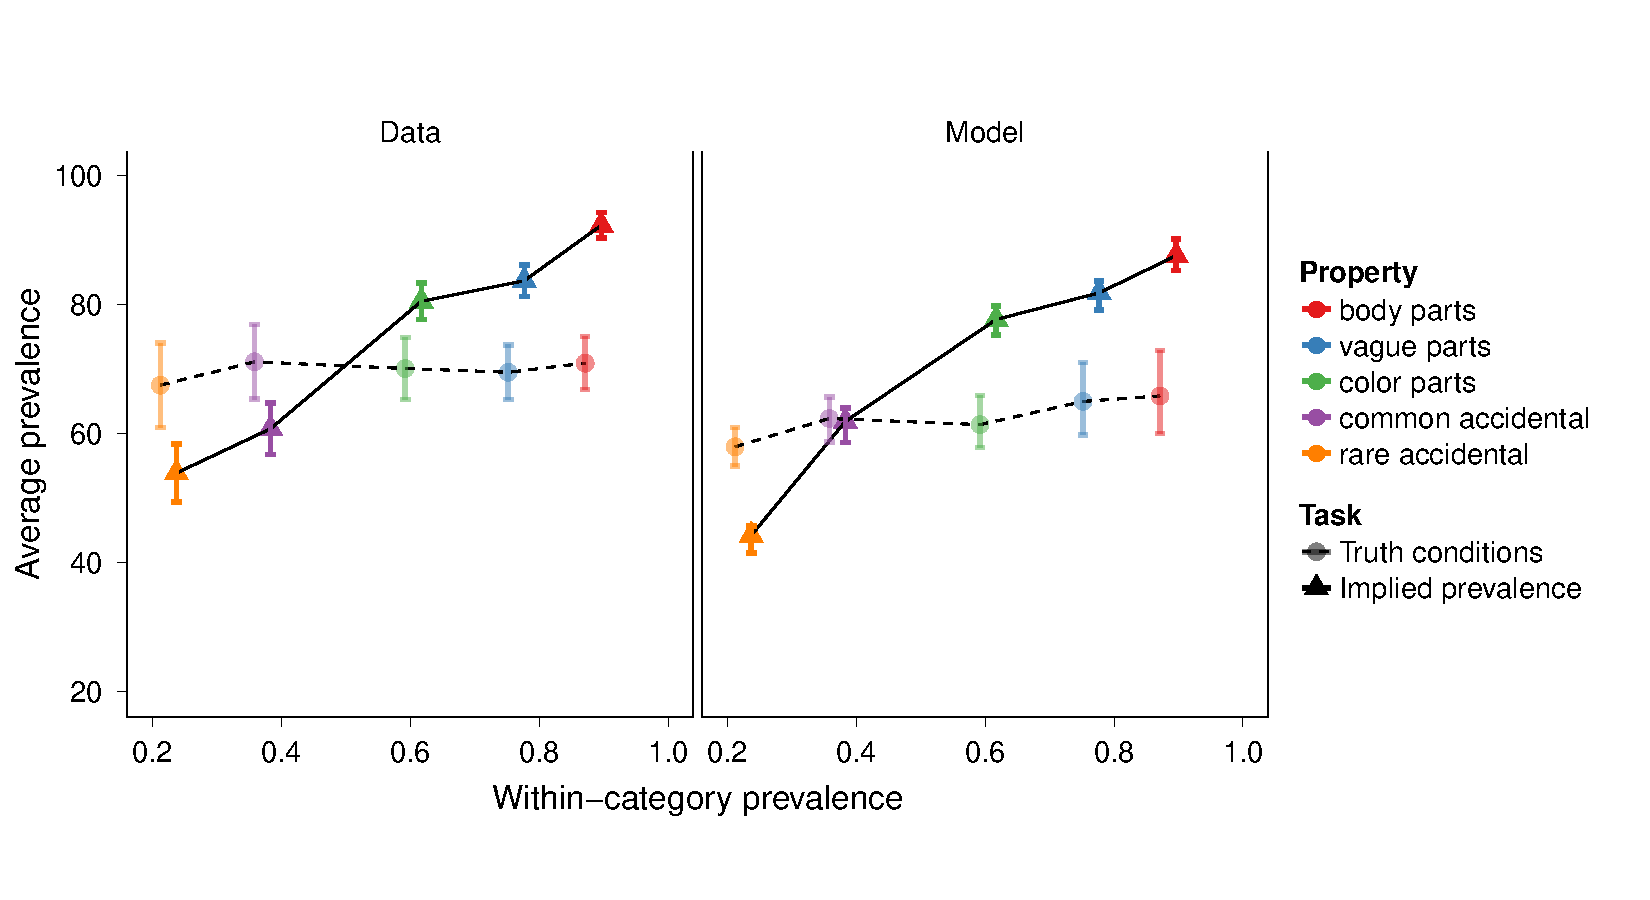
\includegraphics[width=\columnwidth]{asym-lines-data-model-2phi-2so-50kx3.pdf}
%    \includegraphics[width=1.2\columnwidth]{asym-lines-data-model.pdf}
    \caption{Human judgments and model predictions of prevalence implied by novel generic utterances (implied prevalence task; solid line) and average prevalence that leads to an acceptable generic utterance (truth conditions task; dotted line) as it relates to the \emph{a priori} mean prevalence when present $\gamma$.
    Expectations of prevalence are higher after hearing a generic than before hearing it (solid line compared to $y=x$ line; both for human data and model).
    %$y = x$ line denotes the prevalence inferred upon knowing the property is prettyesent in the kind. 
    %For each kind of property, the generic utterance implies a higher than expected prevalence.
    Generic statements about biological properties, imply that the property is widespread in the category, for both human participants and the model (solid line: red, blue and green). 
    Generics about accidental properties do not result in such a high implied prevalence (solid line: purple and orange).  
	While the implications of generic utterances are highly variable across the different types of properties, the average prevalence that leads to an acceptable generic does not vary, for participants or the model.
        %Generic statements are accepted for a range of prevalences, resulting in a intermediate average prevalence (dotted line) that deoesn't vary by property type for the truth conditions task. 
%    Error bars denote bootstrapped 95\% confidence intervals for the data and Bayesian 95\% credible intervals for the model.
%    \ndg{change x-axis label to "a priori expected prevalence" or something like that -- "within-category prevalence" is ambiguous.}
}
  \label{fig:exp2b}
\end{figure*}


%Consistent with the effects reported by \cite{Cimpian2010}, biological properties (body, vague, and color parts) have stronger interpretations than their truth conditions would suggest (Figure \ref{fig:exp2b}; solid vs. dotted lines; green, blue and red points), whereas accidental properties receive more modest interpretations (orange and purple points).



%How does the model capture these fine-grained inferences that listeners draw?
%Consider again the belief distributions about the properties inferred from Expt.~2a (Figure \ref{fig:prior2}). 
%All of the properties have substantial mass at 0 (Figure \ref{fig:prior2} Left). 
%This gives the speaker validity in saying the generic at low prevalence levels (though the speaker's confidence in doing so increases as prevalence increases).
%The listener has the complementary task: She brings \emph{a priori} uncertainty about the generic threshold to the table.
%Consider what would happen if she inferred the most conservative threshold (0) and responded with the \emph{maximum a posteriori} (MAP) of the distribution. 
%A threshold of 0 produces Figure \ref{fig:prior2} (right), because it only rules out the possibility that 0\% of the category has the property. 
%The resulting peaks (MAPs) of the distributions are near 1 for biological properties (parts, color parts, vague parts) and around 10\% for accidental properties (both rare and common). This alone would produce variable interpretations. 
%Our listener, however, does something wiser: She integrates over her uncertainty about the threshold (believing the speaker to be not just truthful but informative as well), and produces interpretations that both take reflect the whole distribution.
%This results in subtle differences between the implications of body parts (e.g. ``Lorches have wings.'') and  color parts (e.g.``Lorches have purple wings.''), and differences in interpretations of rare and common accidental properties. 
%

\section*{Discussion}

We evaluated a theory of generic language derived from general principles of pragmatic language understanding and a simple but uncertain basic meaning---a threshold on property prevalence.
Our formal model is a minimal extension of the RSA theory of language understanding, together with an underspecified threshold semantics.
The model was able to explain two qualitative puzzles of generics: their extremely flexible truth conditions and the contrastingly strong interpretation of novel generics, both of which were revealed to depend in systematic ways on prior knowledge about properties. The model predicted the quantitative details of participants' judgments with high accuracy.

%generics have a simple but uncertain basic meaning---a threshold on property prevalence---which is refined by social reasoning.
%a minimal extension of a general-purpose probabilistic model of language understanding wherein social-cognitive mechanisms act on uncertainty in the meaning of a generic utterance to produce a less uncertain meaning.
%Model predictions for interpretation of generic sentences depend on the listener's beliefs about the property in question and the communicative force of a speech-act. 
%The model predicted participants' judgements with high quantitative accuracy for both goodness judgements for natural generic sentences, and interpretation of novel generic sentences.
%Our model both the role of the speaker to produce felicitous generic utterances and the role of the listener to interpret those utterances in context, with high quantitative accuracy.
%general-purpose language understanding mechanisms are 



%%this paragraph isn't needed and is confusing....
%Interpretation of generic language is strongly governed by listeners' beliefs about the domain in question. 
%The generic, it would seem, doesn't convey any additional information beyond what the liste	ner already knew about the domain.
%This shouldn't surprise us. 
%In much the same way, ``John is tall'' does not actually tell a listener about what \emph{tall} means\footnote{However, ``John is a person'' does tell a listener about what \emph{tall} means in ``John is tall''.}. 
%Rather, the listener is expected to come to the conversation with some beliefs about heights, and knowing that John is a person, be able to infer likely meanings for \emph{tall}.

Previous psychological and philosophical work on generics has looked beyond prevalence and focused on conceptual distinctions and relations \cite{Gelman2005,Prasada2013,Leslie2007,Leslie2008}. 
Prasada et al. has argued for a distinction between \emph{characteristic} properties (e.g.~\emph{Diapers are absorbent.}) and \emph{statistical} properties (e.g.~\emph{Diapers are white.}).
Leslie suggests information that is striking (e.g.~\emph{Tigers eat people.}) is useful and thus permitted to be a generic.
Gelman outlines how generics express \emph{essential} qualities that are relatively timeless and enduring. %,  and that generic language can increase the psychological coherence of a category.
%\citeA{GelmanEtAl2004} finds that child-parent conversations contain many more generics about animal kinds than about artifact kinds, possibly owing to the belief that animal kinds are more richly structured than artifact kinds. 
Where in the prevalence-based semantics could such conceptual distinctions come into play?
Beliefs about prevalence in our approach are represented as probability distributions; a framework that is useful for representing rich, structured knowledge of the world \cite{Goodmanconcepts}. 
Indeed, we found that empirical prevalence distributions are structured, perhaps reflecting intuitions about causal mechanisms underlying different properties.
It is plausible that richer conceptual knowledge also influences these distributions, including higher-order conceptual knowledge about the nature of properties and categories \cite{Gelman2005,Keil1992}. 
However, our approach makes the strong claim that beliefs about prevalence are the connective tissue between conceptual knowledge and generic language.
%may be sufficient to capture truth judgments and interpretations.
%How interlocutors arrive at estimates of the prevalence, and what other inferences are licensed in a context, may be the result of a deeper conceptual model of the world.
That is, the effect of conceptually meaningful differences on generic language is predicted to be mediated by differences in corresponding prevalence distributions.
This suggests a number of further tests of our theory.

To highlight one example, individuals may believe some observations are the result of accidents and are not predictive of future instances (e.g. all of the Supreme Court Justices having even-numbered social security numbers). 
The corresponding generic (i.e. \emph{Supreme Court Justices have even-numbered social security numbers.}) may lack support because the corresponding conceptual models do not have any strong causal mechanism that could have given rise to the observation, and thus the prevalence of the property in the future (i.e. the predictive prevalence) will not be similar to the present prevalence. 
In our experiments, we have focused on properties that are plausibly construed of as essential (e.g. \emph{lays eggs}, \emph{has feathers}) and thus predictive of future instances. 
We found that a set of plausibly temporary properties (e.g. \emph{has muddy feathers}) are interpreted as implying a much lower percentage of the kind with the property than the biological properties, suggestive that the accidental nature of the property influences interpretations of prevalence.


%The results of these studies, as well  future research and model development.

%How interlocutors arrive at estimates of the prevalence, and what other inferences are licensed in a context, may be the result of a deeper conceptual model of the world. 

It might seem paradoxical that a part of language that is so common in communication and central to learning should be vague. 
Shouldn't speakers and teachers want to express their ideas as clearly as possible?
To the contrary, such underspecification can be efficient, given that context can be used to resolve the uncertainty \cite{Piantadosi2012}.
In our work, context takes the form of a listener and speaker's shared beliefs about the property in question. 
By leveraging this common ground, generics provide a powerful way to communicate and learn generalizations about categories, 
which would otherwise be difficult or costly to learn through direct experience.
%This, coupled with standard inferences from conversational pragmatics, allows the listener to arrive at a specific meaning of the otherwise underspecified utterance.
The dark side of this flexibility is the potential for miscommunication or deceit: A speaker might assert a generic utterance that he himself would not accept, conveying a too-strong generalization to a na\"{i}ve listener.  
Our model predicts this potential particularly for properties which, when present, are widespread in a category---we showed that biological properties are believed to have this distribution, but many properties of social categories may as well \cite{Cimpian2011a,Cimpian2012b,Rhodes2012}.
%This listener would then have a belief distribution even further from the truth. 


Categories are inherently unobservable. 
You cannot see the category \textsc{dog}, only some number of instances of it.
Yet we easily talk about these unobservables, conveying hard-won generalizations to each other and down through generations.
The theory presented here gives one explanation of how we do so, providing a computational perspective on how category generalizations are conveyed and how beliefs play a central role in understanding language.






\section*{Materials}
%\begin{materials}
%Details are given in the {\it SI Materials and Methods}.
\subsection{Generics model}
The generics model was implemented using the probabilisitic programming language WebPPL \cite{dippl}. 
The model, once $P(x)$ is fixed, has one free parameter: the speaker rationality parameter $\lambda$ in Eq.~\ref{eq:S1}. 
Because $\lambda$ is not of theoretical interest here, it is marginalized in accord with Bayesian data analysis principles \cite{LW2014}.
Both the prevalence  x$\in$[0, 1]  and the threshold  $\theta \in$[0, 1] were discretized to permit exact enumeration of the posterior.
The prevalence scale was discretized into 11 bins --- \{0, 0.01, 0.1, 0.2, ... , 0.8, 0.9, 0.99\} --- and the threshold scale into 10 bins ---  \{0, 0.1, 0.2, ... , 0.8, 0.9\}. 
The results are the same when a 21, 20 bin discretization is used. 
A fully specified version of the generics model, as well as the structured prior model (described below), can be found at http://forestdb.org/models/generics.html. 








\subsection{Experiment 2a: Prior elicitation for unfamiliar categories}
We recruited 40 participants over MTurk to determine participants' beliefs about the prevalence distribution of novel properties.
%We built on the stimulus set from \cite{Cimpian2010} which consisted of novel animal categories (e.g. \textsc{glippets}) and various properties (e.g. \textsc{have orange legs; have broken legs}).
%To measure the prevalence prior of properties corresponding to \emph{familiar} generics (Expt. 1a), participants filled out a table with rows corresponding to different animal kinds and columns corresponding to different properties. 
%Pilot testing suggested this was a pragmatically strange setup when using novel kinds: answering ``What percentage of lorches have green feathers?'', when participants knew nothing about lorches, was difficult.
We harnessed the latent structure in prevalence priors revealed by Expt.~1a (see main text) to structure our task into 2 questions.
The first question asks how likely it is for there to be a member of \textsc{kind} with \textsc{property}.
The second question asks what percentage of members of \textsc{kind} have \textsc{property}, assuming that there is at least one that does (see {\it SI Section C} for details).
We then used a Bayesian statistical model (described below) to reconstruct the underlying prior distribution. 
%Participants were run through a practice trial where they were familiarized with the questions that would be asked of them. 
%Participants responded using slider bars that ranged from.
%This question aimed to get at the property's potential to be present
%(e.g. it's very likely that there is a glippet that is female, less likely that there is a glippet that has wings, and even less likely that there is a glippet that has purple wings). 
%The question aimed to get at the expected prevalence when present read ``Suppose there is a glippet that has \textsc{property}. What percentage of glippets do you think have \textsc{property}?'' 
%Participants responded using slider bars that ranged from  ``unlikely'' to ``likely'' and from ``0\%'' to ``100\%'', respectively.
%Materials---novel animal names and familiar properties---built upon those from \cite{Cimpian2010}. 
%Classic work in generalization suggested to us that there may be differences in the implications of generic statements of different types of biological properties \cite{Nisbett1983}. 
%We expanded the stimulus set from \cite{Cimpian2010} to include four different types of properties: biological, colored, vague, and accidental body properties / parts. 
%Pilot testing revealed a lot of variability for items in the accidental properties relative to the other types of properties. 
%To test the quantitative predictive power of the generic interpretation model, we used twice as many exemplars of accidental properties, with the aim to make a ``common accidental'' and a ``rare accidental'' class of properties. 
%We used 8 exemplars of each of the three non-accidental properties (``parts'', ``colored parts'', ``vague parts'') and 16 exemplars of accidental properties.
Materials are shown in {\it SI Table 3}.

\subsection{Experiment 2b: Interpretations of novel generics}
We recruited 40 participants over MTurk to determine how widespread different properties are believed to be upon hearing a novel generic.  
%Participants were restricted to those with US IP addresses and with at least a 95\% MTurk work approval rating. 
%All participants were native English speakers. 
%The experiment took about 5 minutes and participants were compensated \$0.60.
%In order to get participants motivated to reason about novel animals, they were told they were the resident zoologist of a team of scientists on a recently discovered island with many unknown animals; their task was to provide their expert opinion on questions about these animals\footnote{The experiment in full can be viewed at \url{http://stanford.edu/~mtessler/generics/experiments/asymmetry/asymmetry-2.html}}. 
%We recruited 40 participants for this \emph{implied prevalence task}. 
Participants were supplied with the generic (e.g. `Glippets have yellow fur.') and asked to judge prevalence: ``What percentage of glippets do you think have yellow fur?''. 
Participants saw 25 trials: 5 for each of 5 property types (see main text and {\it SI Section D}).
%The full cover story is described in {\it SI Section C} and is the same for Expt.~2c.
%The original study by \citeauthor{Cimpian2010} found a difference in the implied prevalence between ``color parts'' (e.g. \textsc{yellow fur}) and accidental properties (e.g. \textsc{wet fur}).
%The prevalence priors inferred from Expt.~2a suggest that generic interpretation could be even more variable.
%For this reason, we included three types of biological properties: parts (e.g. \textsc{fur}), color--part pairs (e.g. \textsc{yellow fur}) and gradable adjective--part pairs (e.g. \textsc{curly fur}). 
%We also coded the accidental properties from Expt.~2a as either ``common'' or ``rare'' using a by-item median split based on \emph{a priori} expected prevalence when present.
%Most of the materials we used were from \citeauthor{Cimpian2010}. 
%The materials used were 30 novel animal categories (e.g. lorches, morseths, blins) each paired with a unique property. 
%Biological properties were made by pairing a color with a body-part (e.g. purple feathers, orange tails). 
%Accidental properties used the same set of body-parts but modified it with an adjective describing an accidental or disease state (e.g. broken legs, wet fur). 
%Each participant saw a random subset of 10 unique animal-property pairs for each type of property (biological and accidental). 

\subsection{Experiment 2c: Asymmetry between interpretations and truth conditions}
%\citeA{Cimpian2010} observed that generic statements of novel kinds with biological properties (e.g. \emph{Glippets have yellow fur.}) show an asymmetry between the conditions by which the generic is true (``\emph{truth conditions}'') and the prevalence implied by the generic (``\emph{implied prevalence}''). 
%Generic sentences were endorsed for a wide-range of prevalence levels (e.g. when ``30\% of glippets have yellow fur.''), resulting in intermediate average truth conditions. 
%As noted above, upon reading a generic, participants inferred that the property was widespread (e.g. almost all glippets have yellow fur).
%This mismatch between \emph{truth conditions} and \emph{implied prevalence} was significantly reduced for generics of properties plausibly construed as accidental (e.g. \emph{Glippets have wet fur.}).
%It was also found to not be present for the quantifier ``most'', arguably the quantifier most similar to a generic.
%This effect was driven by the sensitivity of the implied prevalence metric; the average truth conditions were modulated by the type of property to a much smaller extent.
%
%Below we replicate the asymmetry findings of \citeA{Cimpian2010} and reveal even more variability in the mismatch between \emph{truth conditions} and \emph{implied prevalence} using the types of properties from Expt.~2a.
%Because of the nature of the truth conditions task, our analysis is by property type (as opposed to individual properties as in Expt.~2b).
%
%
%\subsection{Participants}
We recruited 40 participants over MTurk to determine the average prevalence at which a speaker would assert a generic.  
%Participants were restricted to those with US IP addresses and with at least a 95\% MTurk work approval rating. 
%All participants were native English speakers. 
%None of the participants completed Expt.~2b (interpretations of novel generics).
%The experiment took about 5 minutes and participants were compensated \$0.60.
%\subsection{Procedure and materials}
Following Cimpian et al.'s paradigm, participants were given a prevalence statement (e.g.~`30\% of glippets have yellow fur') and asked if they agreed or disagreed with the associated generic statement (i.e.~`Glippets have yellow fur.').
Prevalence varied between 10, 30, 50, 70, and 90\%.
The experiment consisted of 25 trials: 5 trials for each of 5 types of properties measured in Expt.~2a. %(part, color part, vague part, common accidental, rare accidental). 
%Each prevalence level appeared once for each property type (5 prevalence levels x 5 property types). 
%\citeA{Cimpian2010} found that when participants are given statements about prevalence (e.g. ``30\% of lorches have green feathers.'') and asked whether the corresponding generic (e.g. ``Lorches have green feathers'') was true or false, the prevalence on average that participants assented to the generics was reliably less than the prevalence on average that participants inferred upon just reading the generic and being asked about prevalence explicitly. 
%This asymmetry was not present for the quantifier ``most'' (thought to be the most similar quantifier to the generic). 
%For ``most'', participants assented to the generic at an overall average of 75\%, and when told ``Most lorches have green feathers.'', imputed a prevalence of an average 75\%.
%Further, this asymmetry was modulated by the type of property in question. 
%When the property was conceivably biological in nature (e.g. ``green feathers''), the interpretations of generics were much stronger than their average truth conditions.  
%When the property was more accidental in nature (e.g. ``muddy feathers''), this asymmetry disappeared and could presumably reverse.
To compare the truth judgments data (Expt.~2c) to the implied prevalence data (Expt.~2b), we computed, for each subject, an `average prevalence level' that led to ``Agree'' responses, following \cite{Cimpian2010} (see {\it SI Section E} for details).
%For example, if a participant agreed with the generic whenever the prevalence was 70\% or 90\% and disagreed at the other prevalence levels, that participant received an \emph{average prevalence score} of 80\%; if a participant disagreed to everything, their \emph{average prevalence score} was 100\%, since they presumably would only agree with the generic if the prevalence was 100\%.
%We subjected our model to the same procedure. 
%Just as with the experiment with common generics, we use the model of the speaker $S_2$ in Eq.~4 as a model of the \emph{truth conditions} task for novel generics.
%At each prevalence level, the model returns a posterior probability of saying the generic. 
%We take this probability as the parameter of a Bernoulli trial (i.e. as the weight of a coin), and sample a Bernoulli trial (i.e. flip that coin) to predict whether or not the model would agree to the generic for that prevalence level. 
%We then get a sequence of responses corresponding to the responses (\emph{Agree/Disagree}) a participant would give for the 5 different prevalence levels.
%Just as with the human data, we took the \emph{Agree} trials, and took the mean of the prevalence levels corresponding to those \emph{Agree} trials. 
%Thus, we computed the average prevalence at which the model assented to the generic for each property type. 
%We repeated this procedure 40 times to simulate a sample of 40 participants. 
%We repeated this procedure 1000 times to bootstrap 95\% confidence intervals.
%
%\appendix[Structured, Bayesian model of the prior elicitation task]


%\end{materials}
%
%\begin{acknowledgments}
\subsubsection*{Acknowledgements}

This work was supported in part by National Science Foundation Graduate Research Fellowship DGE-114747 (to M.H.T.),
by John S. McDonnell Foundation Scholar Award 220020252 (to N.D.G.) and 
Office of Naval Research Grant N00014-13-1-0788 (to N.D.G.)

%\end{acknowledgments}
%

%\begin{thebibliography}{10}
%
%\bibitem{Carlson1977}
%Carlson GN (1977) Reference to kinds in english, Ph.D. thesis (University of Massachusetts, Amherst).
%
%\bibitem{Leslie2008}
%Leslie SJ (2008) {Generics: Cognition and acquisition}.
%\newblock {\em Philosophical Review} 117(1).
%
%\bibitem{Behrens2005}
%Behrens L (2005) {Genericity from a cross-linguistic perspective}.
%\newblock {\em Linguistics} 43(2):275--344.
%
%\bibitem{Carlson1995}
%Carlson GN, Pelletier FJ (1995) {\em The generic book.}
%\newblock (Chicago University Press).
%
%\bibitem{Gelman2004}
%Gelman SA (2004) {\em Learning words for kinds: Generic noun phrases in
%  acquisition}.
%\newblock (MIT Press), pp. 445--484.
%
%\bibitem{Gelman2008}
%Gelman SA, Goetz PJ, Sarnecka BW, Flukes J (2008) {Generic Language in
%  Parent-Child Conversations}.
%\newblock {\em Language Learning and Development} 4(1):1--31.
%
%\bibitem{Cimpian2008}
%Cimpian A, Markman EM (2008) {Preschool children's use of cues to generic
%  meaning}.
%\newblock {\em Cognition} 107:19--53.
%
%\bibitem{GelmanEtAl2004}
%Gelman SA, Taylor MG, Nguyen SP, Leaper C, Bigler RS (2004) {Mother-child
%  conversations about gender: Understanding the acquisition of essentialist
%  beliefs}.
%\newblock {\em Monographs of the Society for Research in Child Development}
%  69(1):vii, 116--127.
%
%\bibitem{Rhodes2012}
%Rhodes M, Leslie SJ, Tworek CM (2012) {Cultural transmission of social
%  essentialism}.
%\newblock {\em Proceedings of the National Academy of Sciences}
%  109(34):13526--13531.
%
%\bibitem{Leslie2015}
%Leslie SJ, Cimpian A, Meyer M, Freeland E (2015) {Expectations of brilliance
%  underlie gender distributions across academic disciplines}.
%\newblock {\em Science} 347(6219):262--265.
%
%\bibitem{Cimpian2010motivation}
%Cimpian A (2010) {The impact of generic language about ability on children's
%  achievement motivation.}
%\newblock {\em Developmental psychology} 46(5):1333--1340.
%
%\bibitem{Gelman2002}
%Gelman SA, Star JR, Flukes JE (2002) {Children's Use of Generics in Inductive
%  Inferences}.
%\newblock {\em Journal of Cognition and Development} 3(2):179--199.
%
%\bibitem{Cimpian2010}
%Cimpian A, Brandone AC, Gelman SA (2010) {Generic statements require little
%  evidence for acceptance but have powerful implications.}
%\newblock {\em Cognitive science} 34(8):1452--1482.
%
%\bibitem{Brandone2014}
%Brandone AC, Gelman SA, Hedglen J (2014) {Children's Developing Intuitions
%  About the Truth Conditions and Implications of Novel Generics Versus
%  Quantified Statements.}
%\newblock {\em Cognitive science} pp. 1--28.
%
%\bibitem{Carlson1995essay}
%Carlson GN (1995) Truth conditions of generic sentences: Two contrasting views
%  in {\em The Generic Book}, eds.{} Carlson GN, Pelletier FJ.
%\newblock (Univ. of Chicago Press), pp. 224--38.
%
%\bibitem{Prasada2000}
%Prasada S (2000) {Acquiring generic knowledge}.
%\newblock {\em TiCS} 4(2):66--72.
%
%\bibitem{Prasada2012}
%Prasada S, Hennefield L, Otap D (2012) {Conceptual and Linguistic
%  Representations of Kinds and Classes}.
%\newblock {\em Cognitive Science} 36(7):1224--1250.
%
%\bibitem{Clark1996}
%Clark HH (1996) {\em Using language}.
%\newblock (Cambridge University Press).
%
%\bibitem{Grice1975}
%Grice HP (1975) {\em Logic and conversation.}
%\newblock (Blackwell).
%
%\bibitem{Levinson2000}
%Levinson S (2000) {\em Presumptive meanings: The theory of generalized
%  conversational implicature}.
%\newblock (The MIT Press).
%
%\bibitem{Frank2012}
%Frank MC, Goodman ND (2012) Predicting pragmatic reasoning in language games.
%\newblock {\em Science} 336(6084).
%
%\bibitem{Goodman2013}
%Goodman ND, Stuhlm{\"u}ller A (2013) Knowledge and implicature: Modeling
%  language understanding as social cognition.
%\newblock {\em Topics in Cognitive Science}.
%
%\bibitem{Cohen1999}
%Cohen A (1999) {Generics, Frequency Adverbs, and Probability}.
%\newblock {\em Linguistics and Philosophy} 22.
%
%\bibitem{Lassiter2013}
%Lassiter D, Goodman ND (2013) {\em Context, scale structure, and statistics in
%  the interpretation of positive-form adjectives}.
%
%\bibitem{Lassiter2015}
%Lassiter D, Goodman ND (2015) Adjectival vagueness in a bayesian model of
%  interpretation.
%\newblock {\em Synthese}.
%
%\bibitem{Degen2014}
%Degen J, Goodman ND (2014) {\em Lost your marbles? The puzzle of dependent
%  measures in experimental pragmatics}.
%
%\bibitem{Griffiths2005}
%Griffiths TL, Tenenbaum JB (2005) {Structure and strength in causal induction.}
%\newblock {\em Cognitive psychology} 51(4):334--84.
%
%\bibitem{hurdleModels}
%Rose CE, Martin SW, Wannemuehler KA, Plikaytis BD (2006) On the use of
%  zero-inflated and hurdle models for modeling vaccine adverse event count
%  data.
%\newblock {\em Journal of biopharmaceutical statistics} 16(4):463--481.
%
%\bibitem{LW2014}
%Lee MD, Wagenmakers E (2014) {\em Bayesian Cognitive Modeling: A Practical
%  Course}.
%\newblock (Cambridge University Press, Cambridge).
%
%\bibitem{Prasada2013}
%Prasada S, Khemlani S, Leslie SJ, Glucksberg S (2013) {Conceptual distinctions
%  amongst generics.}
%\newblock {\em Cognition} 126(3):405--22.
%
%\bibitem{Nisbett1983}
%Nisbett RE, Krantz DH, Jepson C, Kunda Z (1983) {The use of statistical
%  heuristics in everyday inductive reasoning.}
%\newblock {\em Psychological Review} 90(4):339--363.
%
%\bibitem{Gelman2005}
%Gelman SA (2005) {\em Essential Child: Origins of Essentialism in Everyday
%  Thought.}
%\newblock (Oxford University Press).
%
%\bibitem{Leslie2007}
%Leslie SJ (2007) {Generics and the Structure of the Mind}.
%\newblock {\em Philosophical Perspectives} 21(1):375--403.
%
%\bibitem{Goodmanconcepts}
%Goodman ND, Tenenbaum JB, Gerstenberg T (2015) {\em Concepts in a probabilistic
%  language of thought}.
%\newblock (MIT Press).
%
%\bibitem{Keil1992}
%Keil FC (1992) {\em Concepts, kind, and cognitive development.}
%\newblock (MIT Press).
%
%\bibitem{Piantadosi2012}
%Piantadosi ST, Tily H, Gibson E (2012) {The communicative function of ambiguity
%  in language}.
%\newblock {\em Cognition} 122(3):280--291.
%
%\bibitem{Cimpian2011a}
%Cimpian A, Markman EM (2011) {The Generic/Nongeneric Distinction Influences How
%  Children Interpret New Information About Social Others}.
%\newblock {\em Child Development} 82(2):471--492.
%
%\bibitem{Cimpian2012b}
%Cimpian A, Mu Y, Erickson LC (2012) {Who Is Good at This Game? Linking an
%  Activity to a Social Category Undermines Children's Achievement}.
%\newblock {\em Psychological Science} 23(5):533--541.
%
%\bibitem{dippl}
%Goodman ND, Stuhlm\"{u}ller A (2014) {The Design and Implementation of
%  Probabilistic Programming Languages} (\url{http://dippl.org}).
%\newblock Accessed: 2015-7-17.
%
%\end{thebibliography}

%\end{article}

%\begin{figure*}
%\centering
%    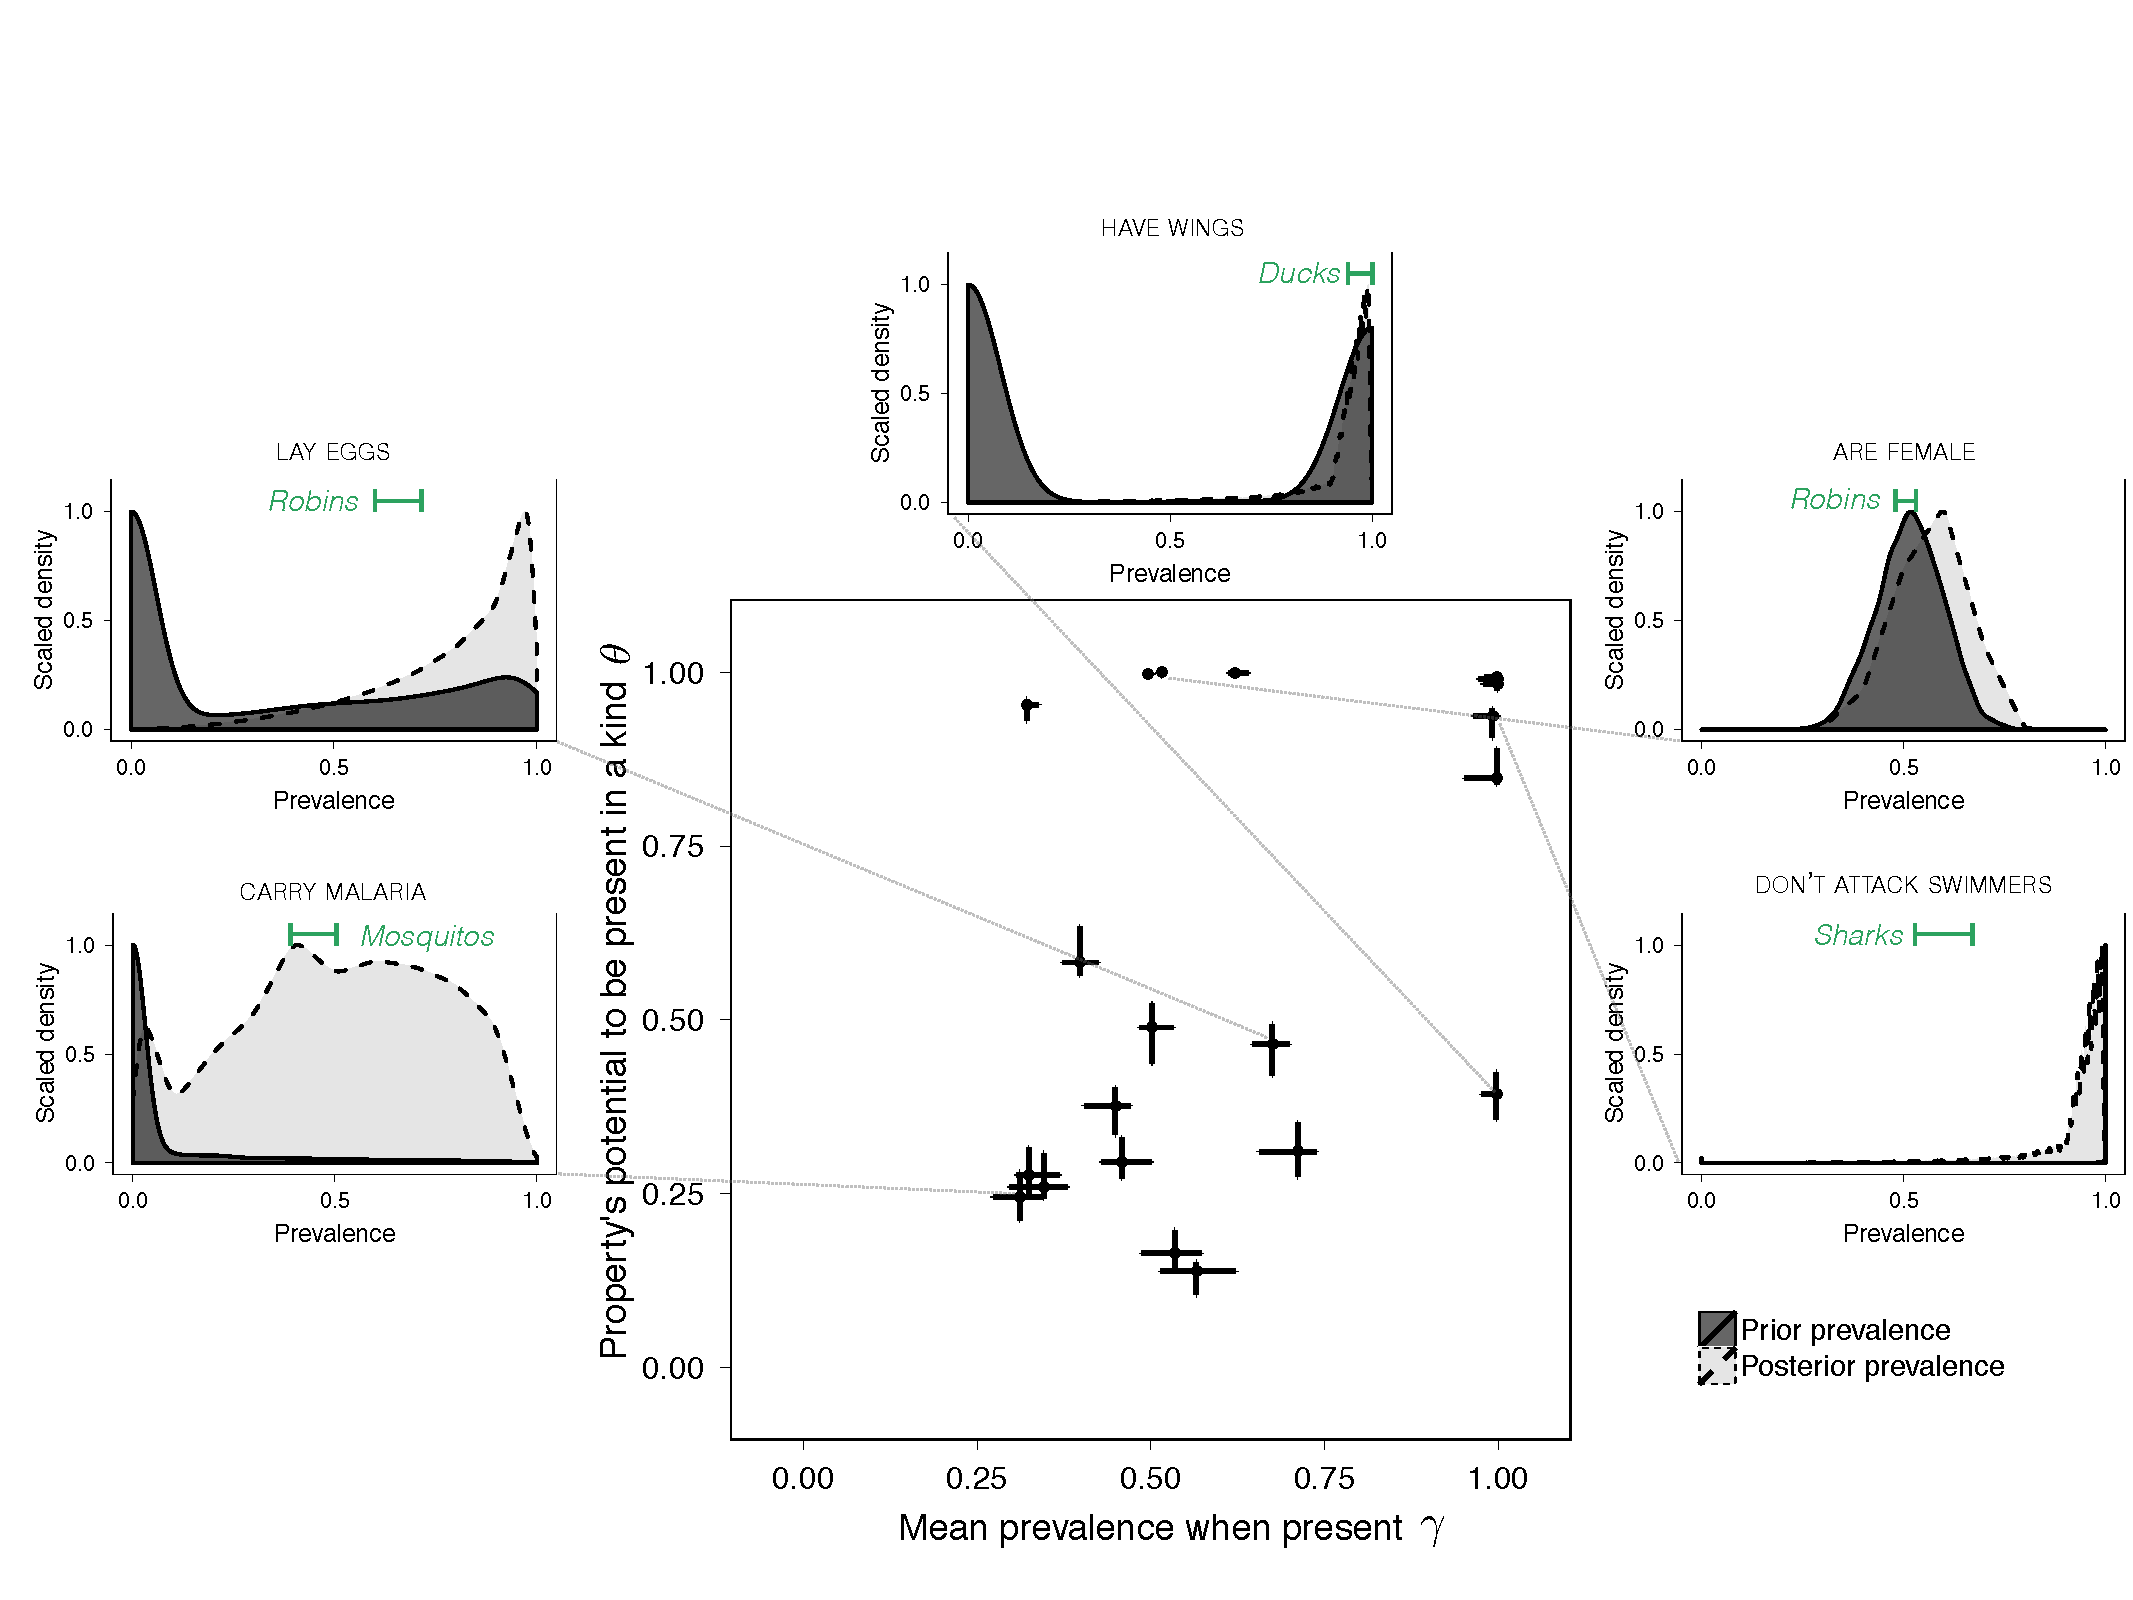
\includegraphics[width=\columnwidth]{prevalence-scatter-wDists2.pdf}
%    \caption{Prevalence prior distributions empirically elicited for twenty-one animal properties.
%    Prior distributions are summarized by $\theta$----a property's potential to be present in a category----and $\gamma$----the mean prevalence when it is possible for the property to be present in a category.
%    Inset plots display example empirical prior distributions over prevalence together with corresponding $L_1$ model predictions: the posterior after hearing a generic utterance. 
%    Intervals on the top of plots show human beliefs about the prevalence of the property within a target category.
%%    Posterior distributions show what happens to a listener's belief about the prevalence after hearing the associated generic. 
%    Felicitous generic utterances result when the target prevalence is more likely under the posterior than under the prior.
% %   \ndg{should mark the observed within-category prevalence for target kinds in pop-outs? or maybe one of the axes of main plot should be that?}
%     Error bars denote 95\% Bayesian credible intervals.
%    }
%  \label{fig:priors1a}
%\end{figure*}
%
%\begin{figure}
%\centering
%    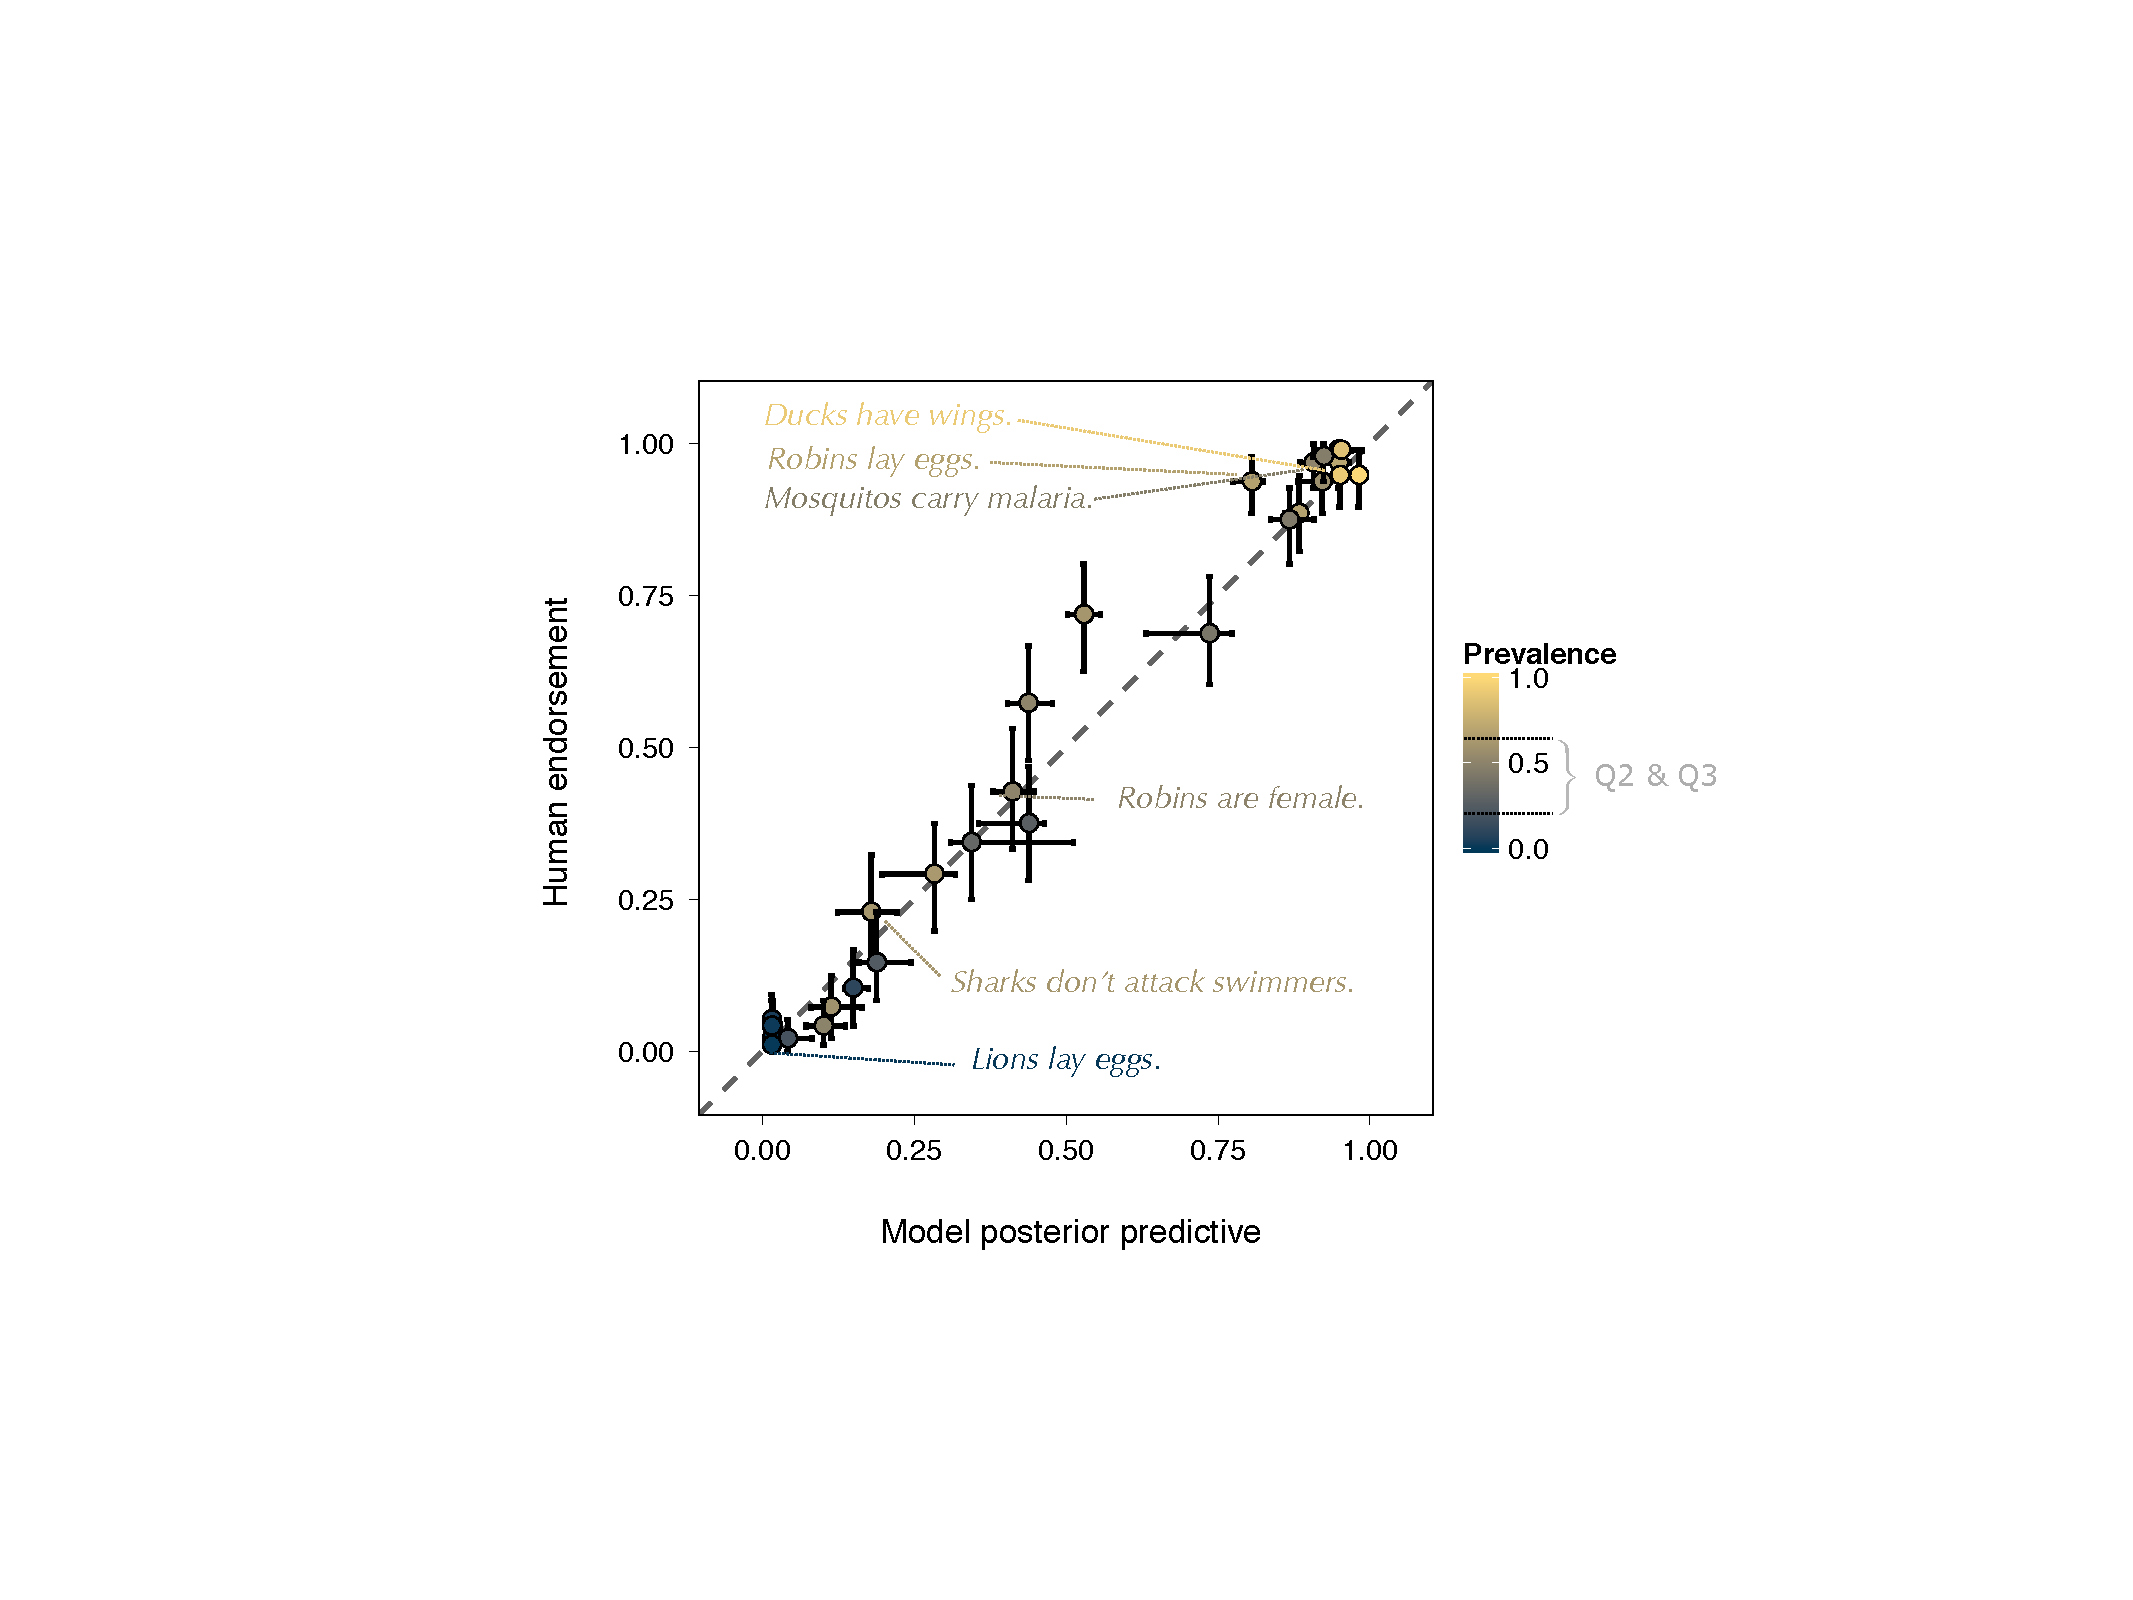
\includegraphics[width=0.49\columnwidth]{truthjudge-scatter-wLabels.pdf}
%    \caption{Human acceptability judgments and model predictions for thirty generic utterances about familiar animals and properties. 
%    Color denotes target-category prevalence of the property, with darker colors indicating lower prevalence. 
%    Intermediate prevalences (quartiles 2 \& 3) are in intermediate shades (marked on color bar).
%    Error bars correspond with 95\% bootstrapped confidence intervals for the participant data and 95\% highest probability intervals for the model predictions.
%    }
%  \label{fig:modeldataBars}
%\end{figure}
%
%
%\begin{figure*}
%\centering
%    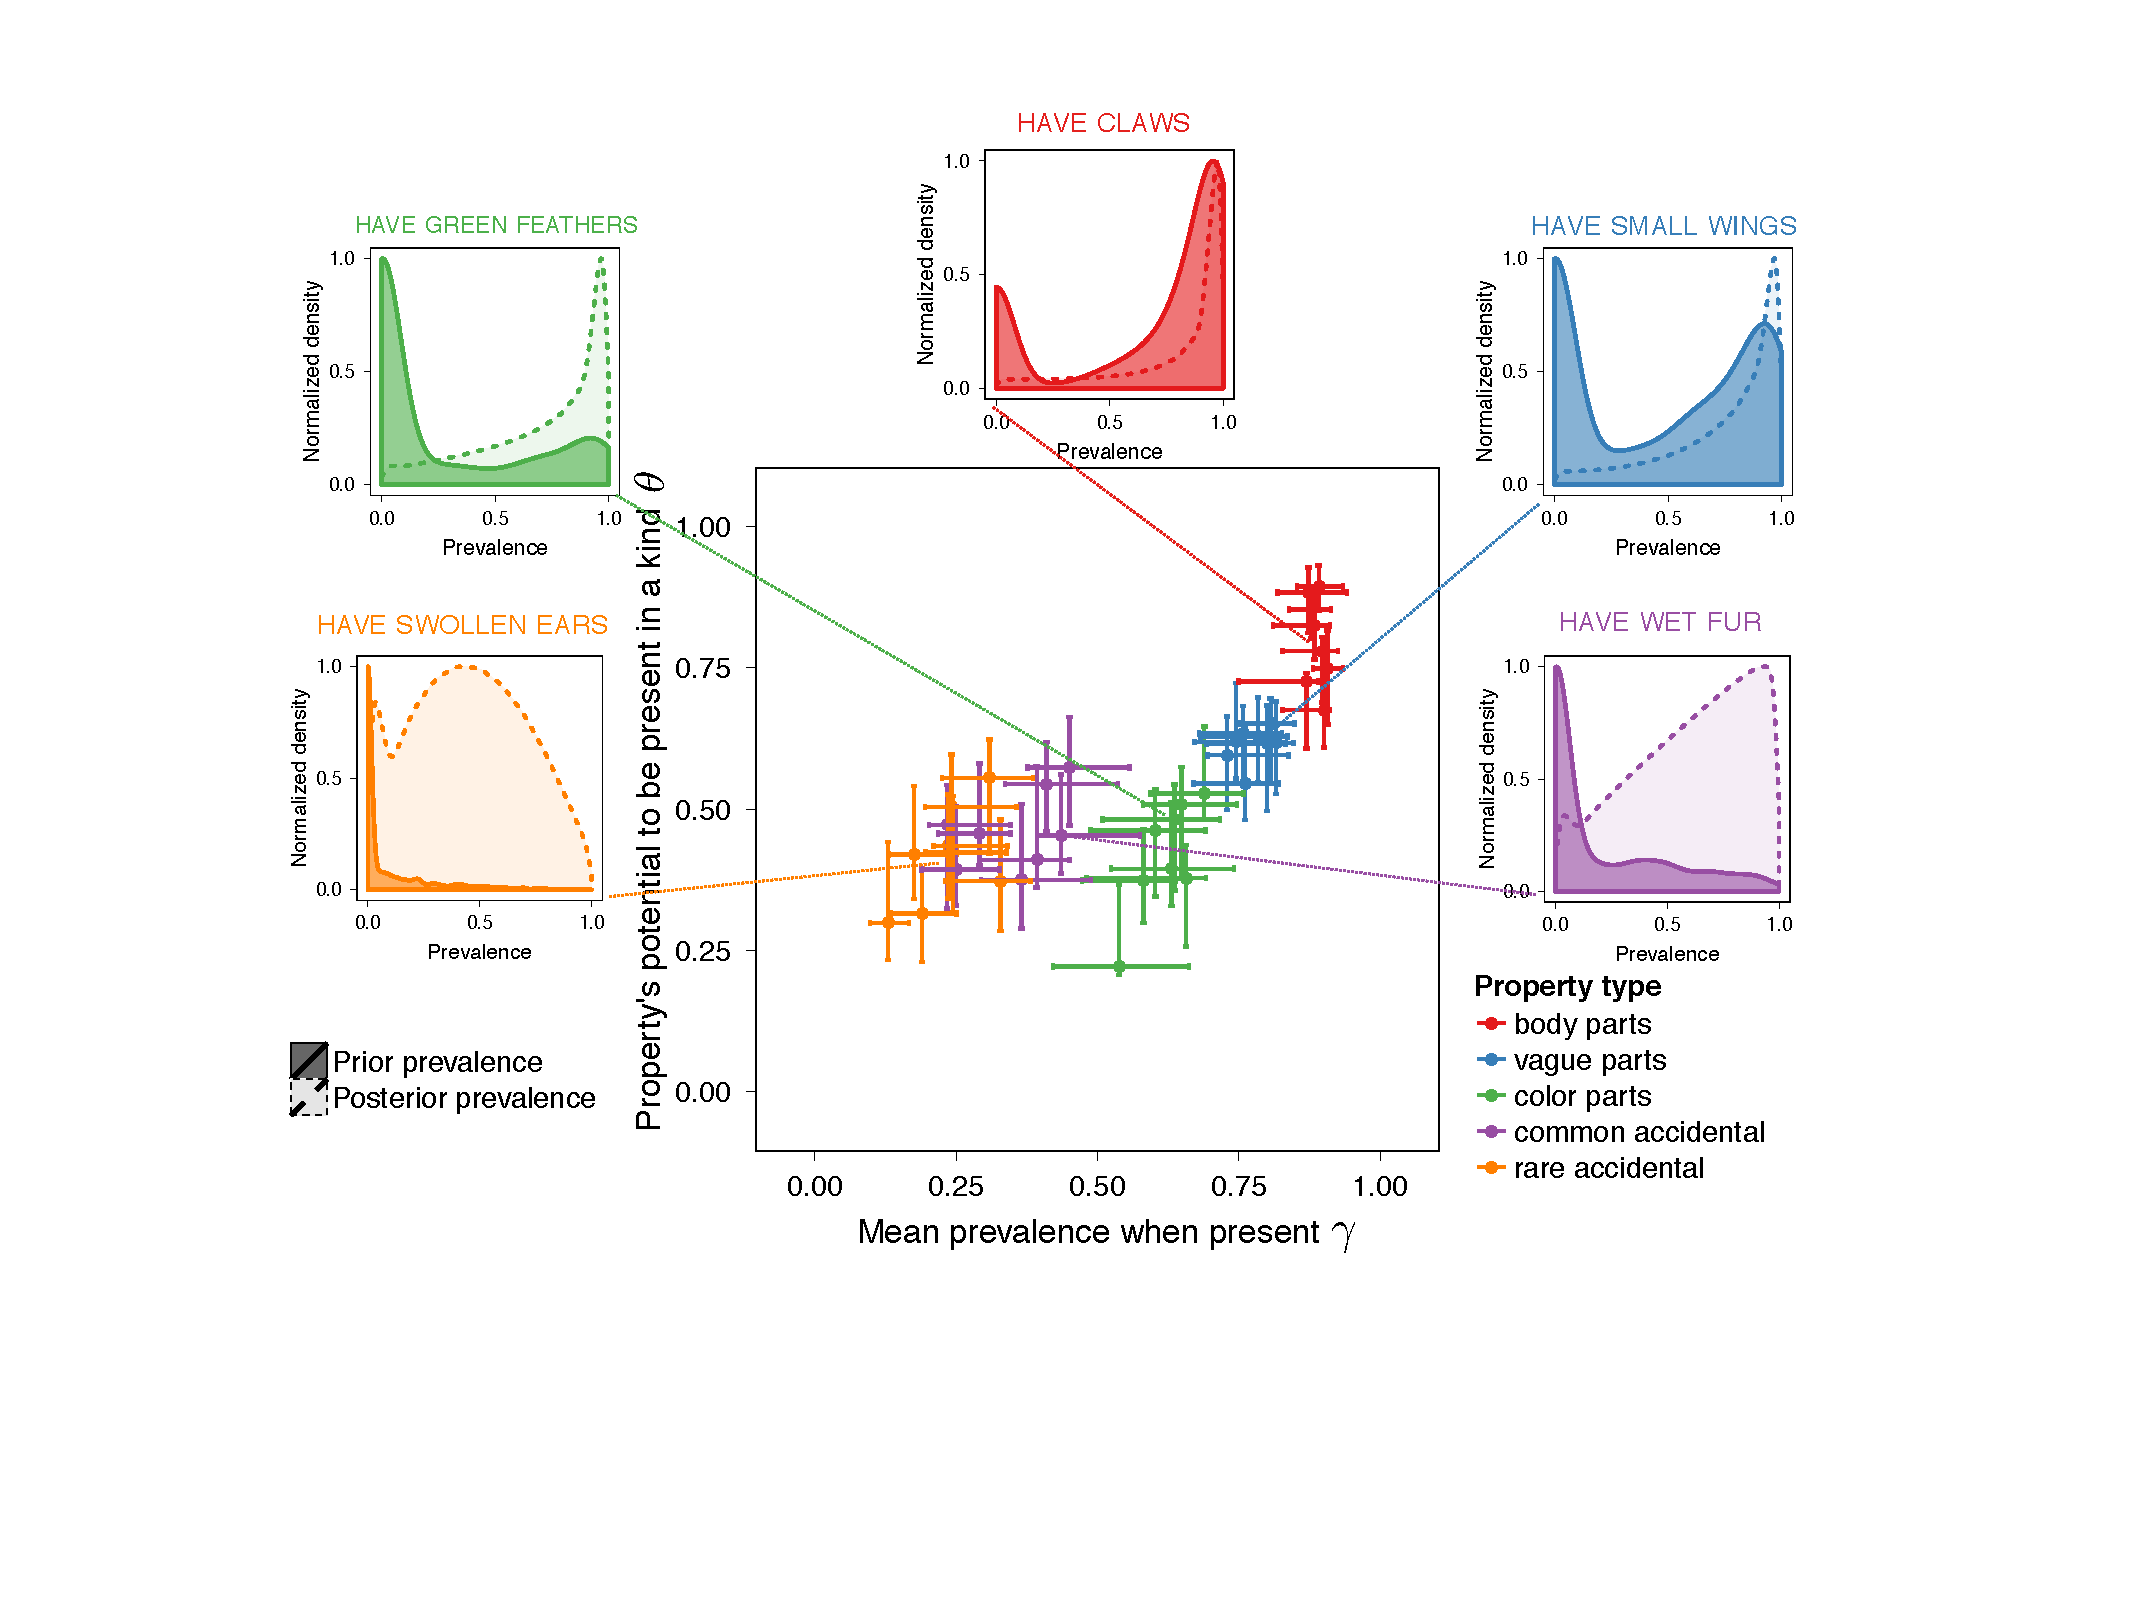
\includegraphics[width=\columnwidth]{prevalence-asymmetry-scatterwDists-byItem.pdf}
%    \caption{Prevalence prior distributions empirically elicited for 40 animal properties.
%    Parameters of the structured statistical model---$\theta$ and $\gamma$---reveal quantitative differences in beliefs about the prevalence of conceptually different types of properties (scatterplot). 
%    Inset plots show differences in shapes between biological properties (red, green, blue; bimodal) and accidental properties (orange, purple; unimodal).   
%  These differences give rise to the variability of interpretations of generic utterances. 
%      Error bars denote Bayesian 95\% credible intervals.
%  }
%  \label{fig:prior2}
%\end{figure*}
%
%
%\begin{figure}
%\centering
%    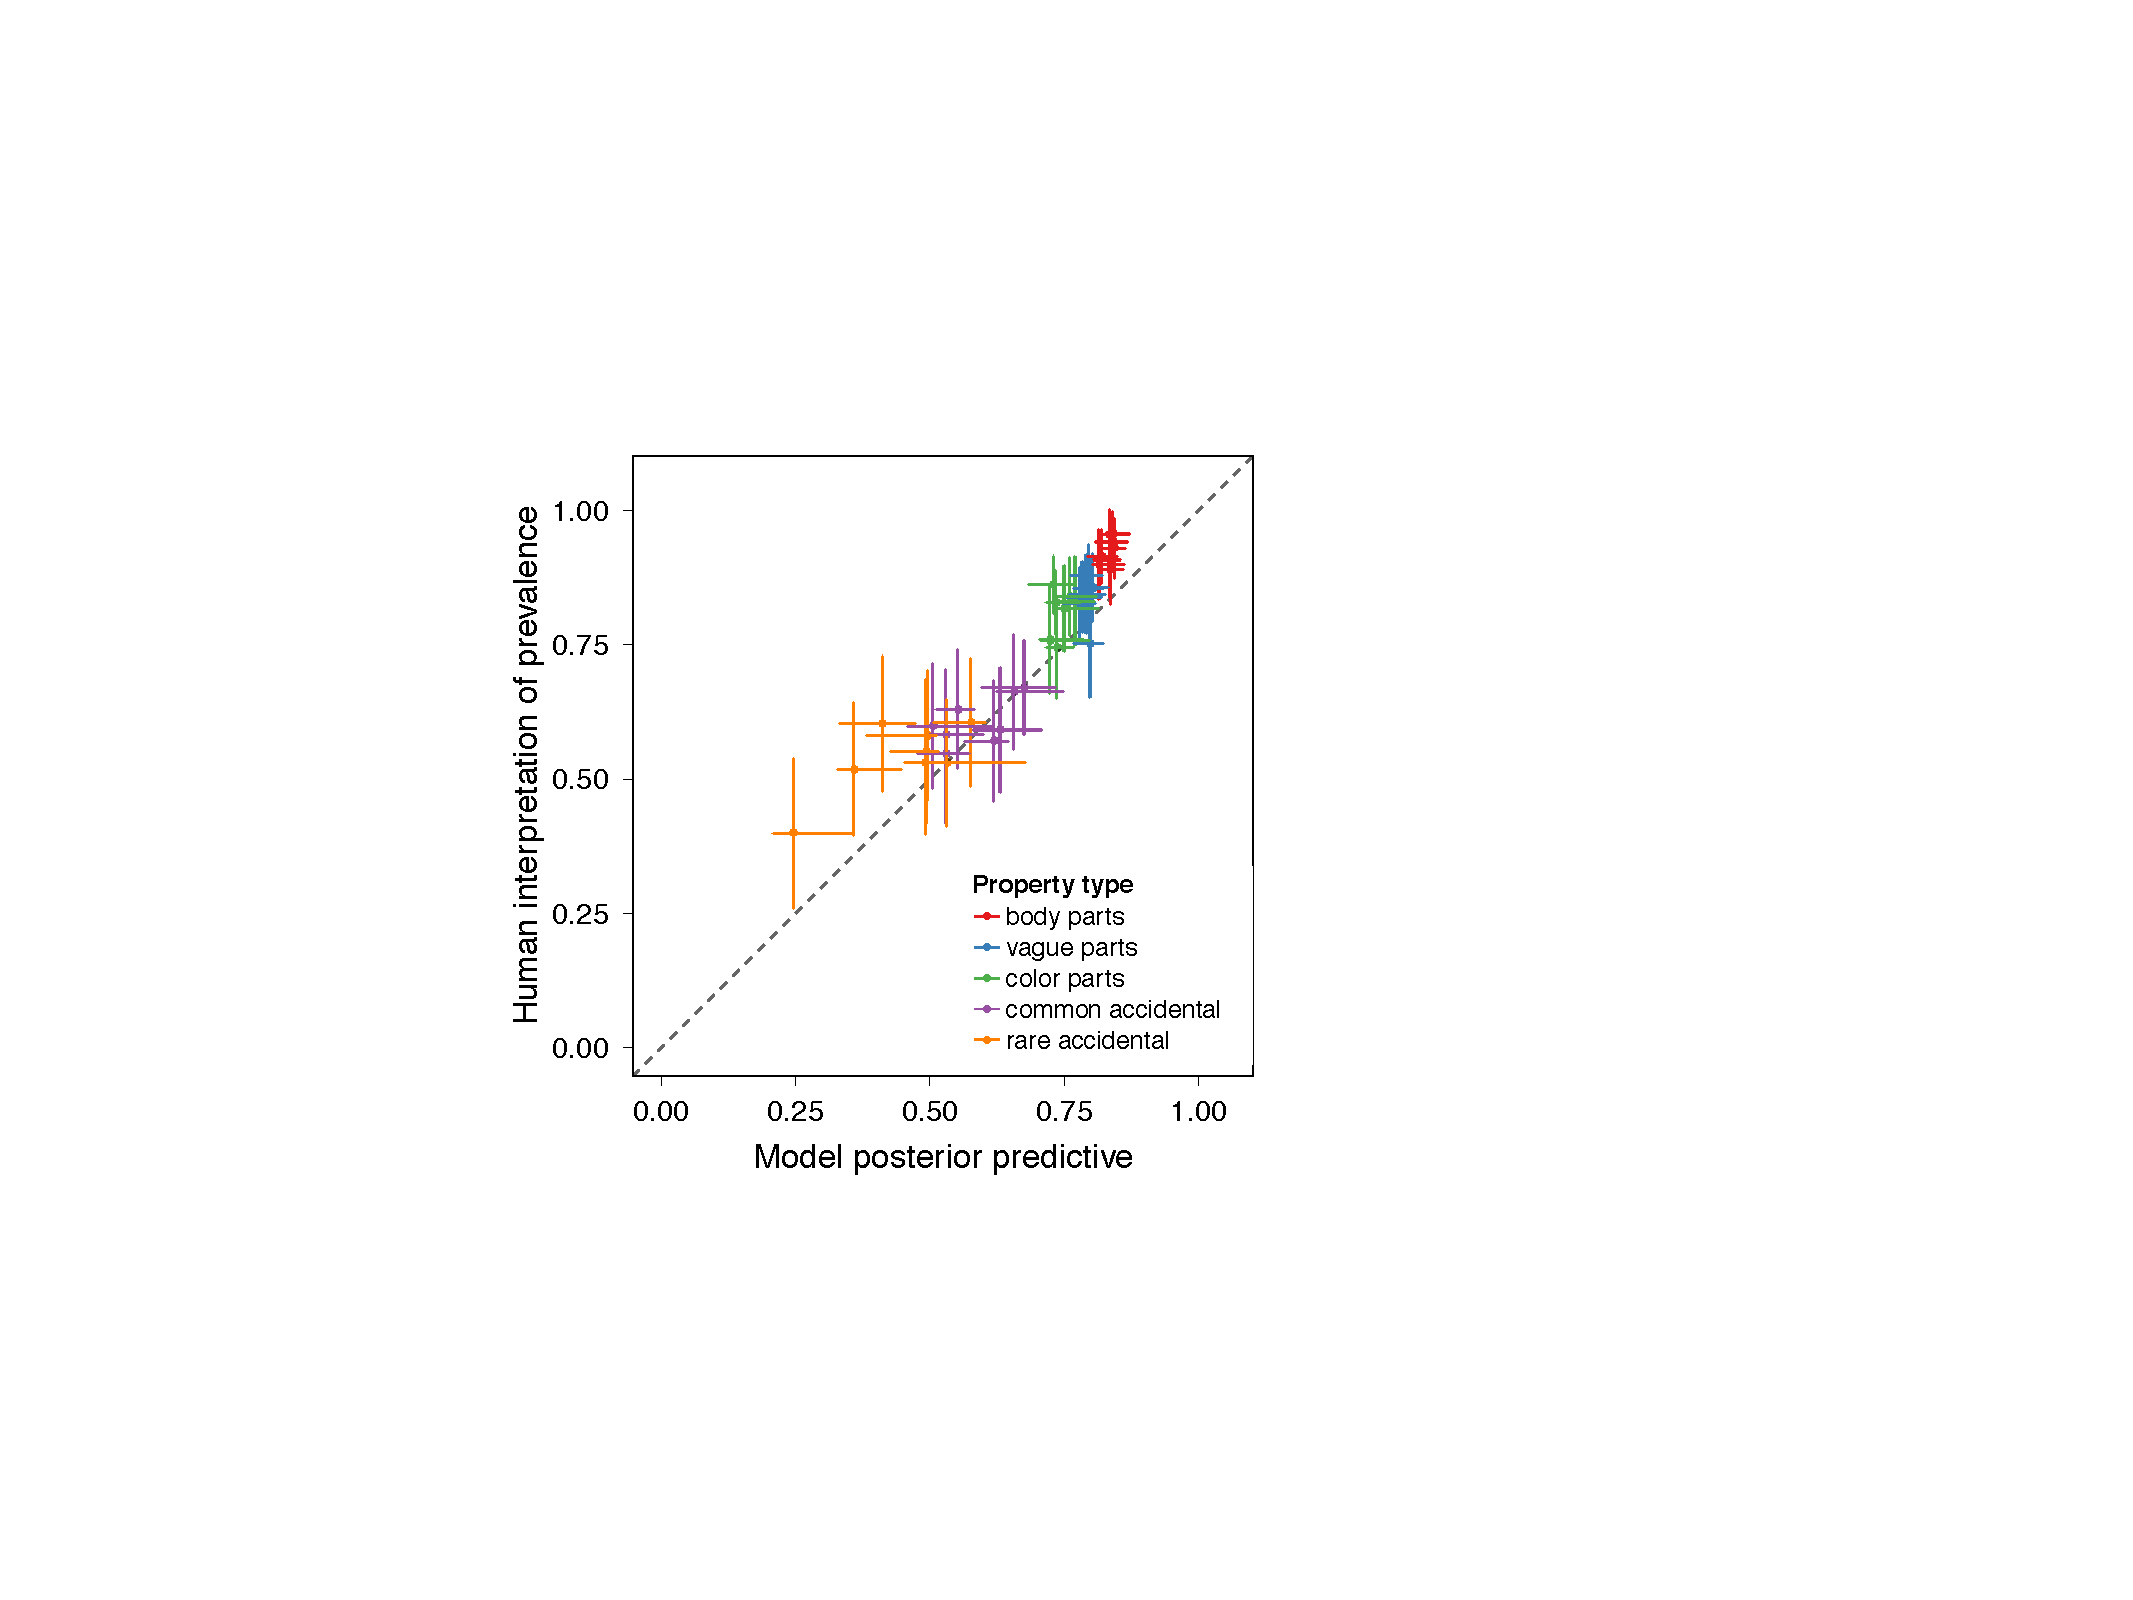
\includegraphics[width=0.48\columnwidth]{implied-byItem-mh100kX2b.pdf}
%    \caption{Human interpretation of prevalence upon hearing a generic compared with the $L_1$ model posterior predictive. 
%    Participants display graded endorsements of generics in terms of prevalence based on type of property (which is also associated with \emph{mean prevalence when present} $\gamma$, see Figure 3).
%    The model displays the same variability of interpretation, producing strong interpretations for generics of biological properties (red, blue, green) and weaker interpretations of generics of accidental properties (purple, orange).
%        Error bars denote bootstrapped 95\% confidence intervals for the data and Bayesian 95\% credible intervals for the model.}
%  \label{fig:impliedByItem}
%\end{figure}
%
%\begin{figure*}
%\centering
%    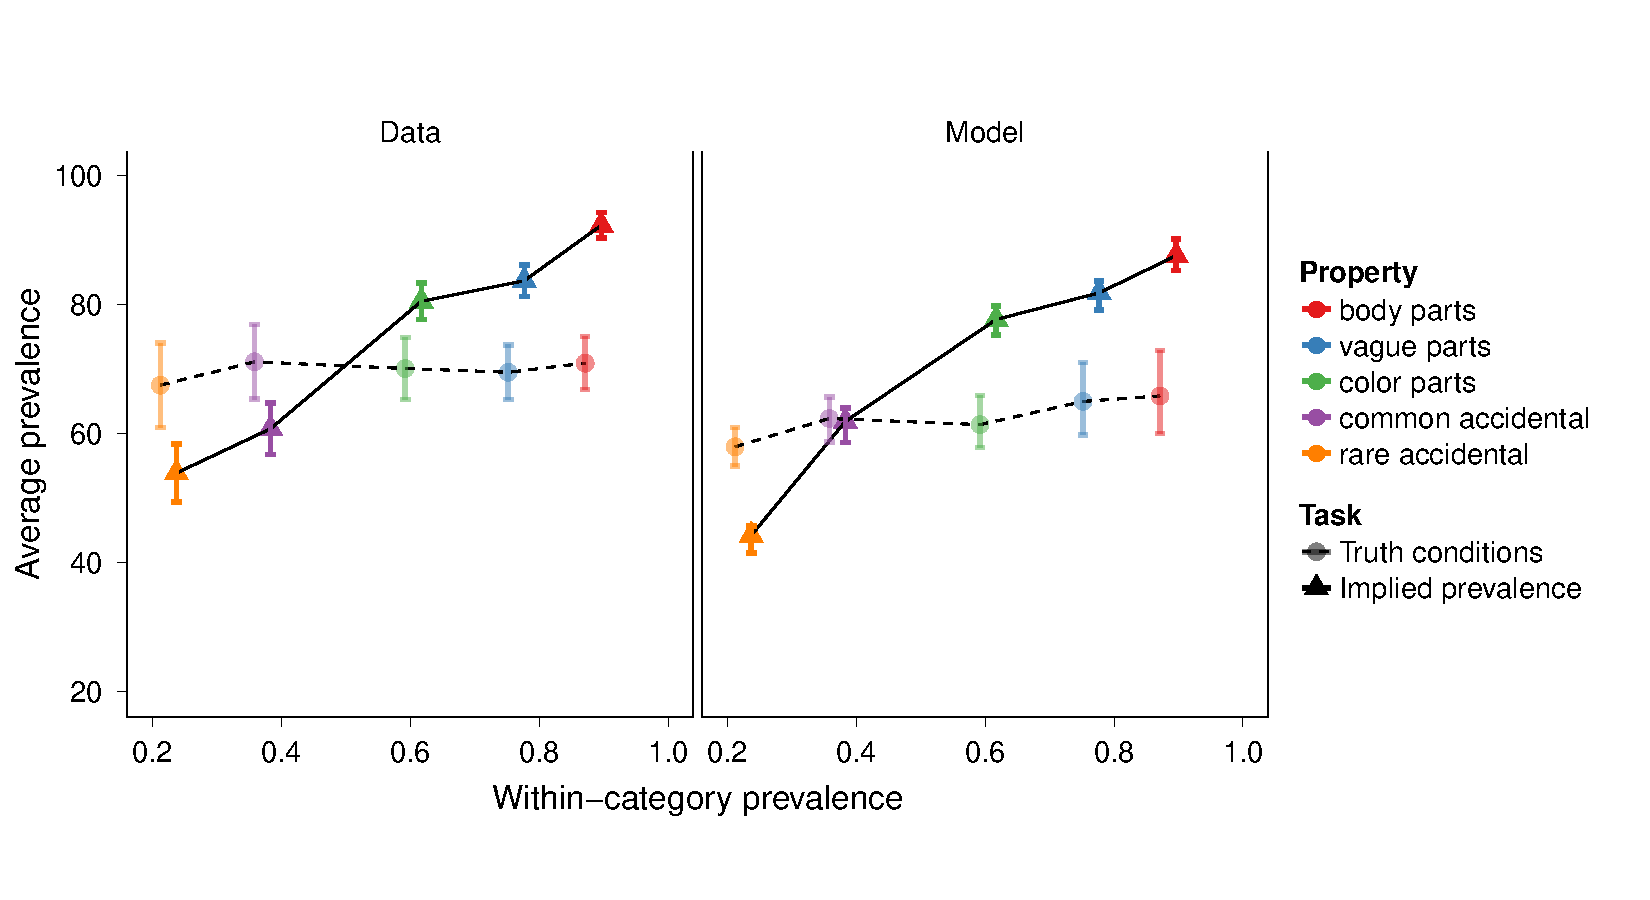
\includegraphics[width=\columnwidth]{asym-lines-data-model-2phi-2so-50kx3.pdf}
%    \caption{Human judgments and model predictions of prevalence implied by novel generic utterances (implied prevalence task; solid line) and average prevalence that leads to an acceptable generic utterance (truth conditions task; dotted line) as it relates to the \emph{a priori} mean prevalence when present $\gamma$.
%    Expectations of prevalence are higher after hearing a generic than before hearing it (solid line compared to $y=x$ line; both for human data and model).
%    %$y = x$ line denotes the prevalence inferred upon knowing the property is prettyesent in the kind. 
%    %For each kind of property, the generic utterance implies a higher than expected prevalence.
%    Generic statements about biological properties, imply that a high proportion of the category has the property, for both human participants and the model (solid line: red, blue and green). 
%    Generics about accidental properties do not result in such a high implied prevalence (solid line: purple and orange).  
%	While the implications of generic utterances are highly variable across the different types of properties, the average prevalence that leads to an acceptable generic does not vary, for participants or the model.
%        %Generic statements are accepted for a range of prevalences, resulting in a intermediate average prevalence (dotted line) that deoesn't vary by property type for the truth conditions task. 
%    Error bars denote bootstrapped 95\% confidence intervals for the data and Bayesian 95\% credible intervals for the model.
%%    \ndg{change x-axis label to "a priori expected prevalence" or something like that -- "within-category prevalence" is ambiguous.}
%}
%  \label{fig:exp2b}
%\end{figure*}

\bibliographystyle{apacite}

\setlength{\bibleftmargin}{.125in}
\setlength{\bibindent}{-\bibleftmargin}

\bibliography{generics}

\end{document}


